\documentclass[11pt,a4paper,twoside,openright]{book}
\usepackage[utf8]{inputenc}
\usepackage[T1]{fontenc}
%\usepackage{lipsum}% juste utile ici pour générer du faux texte}
\usepackage{mwe}%juste utile ici pour générer de fausses images
\usepackage{amsmath,amsfonts,amssymb}%extensions de l'ams pour les mathé matiques
\usepackage{shorttoc}%pour la réalisation d'un sommaire.
\usepackage{tikz}
\usepackage{graphicx}%pour insérer images et pdf entre autres
	\graphicspath{{images/}}%pour spécifier le chemin d'accès aux images
\usepackage{pdfpages}
\usepackage{geometry}%réglages des marges du document selon vos préférences ou celles de votre établissemant[left=3.5cm,right=2.5cm,top=4cm,bottom=4cm]
\usepackage[Lenny]{fncychap}%pour de jolis titres de chapitres voir la doc pour d'autres styles.

\usepackage{fancyhdr}%pour les entêtes et pieds de pages
	\setlength{\headheight}{14.2pt}% hauteur de l'entête

%%%%%%%%%%%%%%%%%%%style front%%%%%%%%%%%%%%%%%%%%%%%%%%%%%%%%%%%%%%%%%	
	\fancypagestyle{front}{%
  		\fancyhf{}%on vide les entêtes
  		\fancyfoot[C]{page \thepage}%
  		\renewcommand{\headrulewidth}{0pt}%trait horizontal pour l'entête
  		\renewcommand{\footrulewidth}{0.4pt}%trait horizontal pour les pieds de pages
		}


%%%%%%%%%%%%%%%%%%%style main%%%%%%%%%%%%%%%%%%%%%%%%%%%%%%%%%%%%
	\fancypagestyle{main}{%
		\fancyhf{}
  		\renewcommand{\chaptermark}[1]{\markboth{\chaptername\ \thechapter.\ ##1}{}}% redéfintion pour avoir ici les titres des chapitres des sections en minuscules
  		\renewcommand{\sectionmark}[1]{\markright{\thesection\ ##1}}
		\fancyhead[c]{}
		\fancyhead[RO,LE]{\rightmark}%
  		\fancyhead[LO,RE]{\leftmark}
		\fancyfoot[C]{}
		\fancyfoot[RO,LE]{page \thepage}%
  		%\fancyfoot[LO,RE]{Rapport de contrat de professionnalisation}
  		}

%%%%%%%%%%%%%%%%%%%style back%%%%%%%%%%%%%%%%%%%%%%%%%%%%%%%%%%%%%%%%%	
	\fancypagestyle{back}{%
  		\fancyhf{}%on vide les entêtes
  		\fancyfoot[C]{page \thepage}%
  		\renewcommand{\headrulewidth}{0pt}%trait horizontal pour l'entête
  		\renewcommand{\footrulewidth}{0.4pt}%trait horizontal pour les pieds de pages
		}


%%%%%%%%%%%%%%%%%%%%%%%%%%%%index%%%%%%%%%%%%%%%%%%%%%%%%%%%%%%%%%%%%%%%
\usepackage{makeidx}
%\usepackage{xindy}
\makeindex




%\usepackage[thinlines]{easytable}
%\usepackage{changepage}
%\usepackage{fullwidth}


%\DeclareUnicodeCharacter{00A0}{~}



%\usepackage{newunicodechar}
%\newunicodechar{^^a0}{~}


\usepackage{listings}
\usepackage{color}
\definecolor{mygreen}{rgb}{0,0.6,0}
\definecolor{mygray}{rgb}{0.5,0.5,0.5}
\definecolor{mymauve}{rgb}{0.58,0,0.82}
\lstset{ %
  backgroundcolor=\color{white},   % choose the background color; you must add \usepackage{color} or \usepackage{xcolor}
  basicstyle={\small\ttfamily},        % \footnotesize : the size of the fonts that are used for the code
  breakatwhitespace=false,         % sets if automatic breaks should only happen at whitespace
  breaklines=true,                 % sets automatic line breaking
  captionpos=none,                    % b : sets the caption-position to bottom
  commentstyle=\color{mygreen},    % comment style
  deletekeywords={...},            % if you want to delete keywords from the given language
  escapeinside={\%*}{*)},          % if you want to add LaTeX within your code
  extendedchars=true,              % lets you use non-ASCII characters; for 8-bits encodings only, does not work with UTF-8
  frame=none,	                   % single : adds a frame around the code
	% tb : 
  keepspaces=true,                 % keeps spaces in text, useful for keeping indentation of code (possibly needs columns=flexible)
	columns=flexible,
  keywordstyle=\color{blue},       % keyword style
  %language=Java,                 % the language of the code
  otherkeywords={*,...},            % if you want to add more keywords to the set
  numbers=left,                    % where to put the line-numbers; possible values are (none, left, right)
  numbersep=5pt,                   % how far the line-numbers are from the code
  numberstyle=\tiny\color{mygray}, % the style that is used for the line-numbers
  rulecolor=\color{black},         % if not set, the frame-color may be changed on line-breaks within not-black text (e.g. comments (green here))
  showspaces=false,                % show spaces everywhere adding particular underscores; it overrides 'showstringspaces' <=> showstringspaces=false
  showstringspaces=false,          % underline spaces within strings only
  showtabs=false,                  % show tabs within strings adding particular underscores
  stepnumber=2,                    % the step between two line-numbers. If it's 1, each line will be numbered
  stringstyle=\color{mymauve},     % string literal style
  tabsize=2,	                   % sets default tabsize to 2 spaces
  title=\lstname,                   % show the filename of files included with \lstinputlisting; also try caption instead of title
	aboveskip=3mm,
  belowskip=3mm
}



\usepackage{textcomp}%  \texttildelow

\usepackage[english,french]{babel}%pour un document en français
\usepackage{hyperref}%rend actif les liens, références croisée, toc, ...
		\hypersetup{colorlinks,%
		citecolor=black,%
		filecolor=black,%
		linkcolor=black,%
		urlcolor=black} 
%%%%%%%%%%%%%%%%%%%%%%%%%%%%biblio%%%%%%%%%%%%%%%%%%%%%%%%%%%%%%%%%%%%%%
\usepackage[backend=biber]{biblatex}
\addbibresource{bibliographie/biblio.bib}% pour indiquer ou se trouve notre .bib
\usepackage{csquotes}% pour la gestion des guillemets français.

%%%%%%%%%%%%%%%%%%%%%%%%%%%%%glossaire%%%%%%%%%%%%%%%%%%%%%%%%%%%%%%%%%%%
\usepackage{glossaries}
\makeglossaries		

%%%%%%%%%%%%%%%%%%%%%%%%%%%%liste des abbréviations%%%%%%%%%%%%%%		
\usepackage[french]{nomencl}
\makenomenclature
\renewcommand{\nomname}{Liste des abréviation, des sigles et des symboles}

%\glsresetall
%\glsaddall


%Please load the package listings after 'babel'
\usepackage{listings}
\usepackage{color}
\definecolor{mygreen}{rgb}{0,0.6,0}
\definecolor{mygray}{rgb}{0.5,0.5,0.5}
\definecolor{mymauve}{rgb}{0.58,0,0.82}
\lstset{ %
  backgroundcolor=\color{white},   % choose the background color; you must add \usepackage{color} or \usepackage{xcolor}
  basicstyle={\small\ttfamily},        % \footnotesize : the size of the fonts that are used for the code
  breakatwhitespace=false,         % sets if automatic breaks should only happen at whitespace
  breaklines=true,                 % sets automatic line breaking
  captionpos=none,                    % b : sets the caption-position to bottom
  commentstyle=\color{mygreen},    % comment style
  deletekeywords={...},            % if you want to delete keywords from the given language
  escapeinside={\%*}{*)},          % if you want to add LaTeX within your code
  extendedchars=true,              % lets you use non-ASCII characters; for 8-bits encodings only, does not work with UTF-8
  frame=none,	                   % single : adds a frame around the code
	% tb : 
  keepspaces=true,                 % keeps spaces in text, useful for keeping indentation of code (possibly needs columns=flexible)
	columns=flexible,
  keywordstyle=\color{blue},       % keyword style
  language=Java,                 % the language of the code
  otherkeywords={*,...},            % if you want to add more keywords to the set
  numbers=left,                    % where to put the line-numbers; possible values are (none, left, right)
  numbersep=5pt,                   % how far the line-numbers are from the code
  numberstyle=\tiny\color{mygray}, % the style that is used for the line-numbers
  rulecolor=\color{black},         % if not set, the frame-color may be changed on line-breaks within not-black text (e.g. comments (green here))
  showspaces=false,                % show spaces everywhere adding particular underscores; it overrides 'showstringspaces' <=> showstringspaces=false
  showstringspaces=false,          % underline spaces within strings only
  showtabs=false,                  % show tabs within strings adding particular underscores
  stepnumber=2,                    % the step between two line-numbers. If it's 1, each line will be numbered
  stringstyle=\color{mymauve},     % string literal style
  tabsize=2,	                   % sets default tabsize to 2 spaces
  title=\lstname,                   % show the filename of files included with \lstinputlisting; also try caption instead of title
	aboveskip=3mm,
  belowskip=3mm
}


\makeatletter
\newenvironment{abstract}{%
    \cleardoublepage
    \null\vfil
    \@beginparpenalty\@lowpenalty
    \begin{center}%
      \bfseries \abstractname
      \@endparpenalty\@M
    \end{center}}%
   {\par\vfil\null}
\makeatother




\newglossaryentry{pois}{name={poisson},description={Les poissons sont des animaux vertébrés aquatiques à branchies, pourvus de nageoires et dont le corps est le plus souvent couvert d'écailles.}}

\newglossaryentry{vache}{name={vache},description={Vache est le nom vernaculaire donné à la femelle du taureau et à la mère du veau des bovins.}}

\newglossaryentry{pigeon}{name={pigeon},description={Les pigeons sont des oiseaux de la famille des Columbidae.}}


\newacronym{lvm}{LVM}{Logical Volume Manager}
\newacronym{TEM}{TEM}{scanning electron microscope}


\newglossaryentry{latex}
{
    name=latex,
    description={Is a mark up language specially suited 
    for scientific documents}
}

\begin{document}
\frenchspacing
\frontmatter% début des pages liminaires
\pagestyle{front}%style des entêtes pour cette partie
%
\newgeometry{left=1.5cm,right=1.5cm,top=1.5cm,bottom=1.5cm}
\begin{titlepage}
\parindent=0pt

ESIGELEC \hspace*{\stretch{1}} Pierre TAQUET

Saint-Etienne du Rouvray (76)

\vspace*{\stretch{1}}

\includegraphics[width=0.5\textwidth]{images/ESIGELEC.jpg}
\hspace*{\stretch{1}}

\includegraphics[height=75px]{images/SAP.png}
\vspace*{\stretch{2}}

\rule{\textwidth}{1.6pt}\vspace*{-\baselineskip}\vspace*{2pt} % Thick horizontal line
\rule{\textwidth}{0.4pt}% Thin horizontal line
\begin{center}\bfseries\Huge
Contrat de professionnalisation
\end{center}
\hrulefill
\begin{center}\bfseries\LARGE
\'{E}quipe ST Automation
\end{center}
\rule{\textwidth}{0.4pt}\vspace*{-\baselineskip}\vspace{3.2pt} % Thin horizontal line
\rule{\textwidth}{1.6pt}\\[\baselineskip] % Thick horizontal line

\vspace*{\stretch{1}} 
		
%\begin{center}\bfseries\Large
%Sous la direction de Le Tuteur.
%\end{center}

\vspace*{\stretch{2}}

\begin{table}[b!]
\begin{center}
\begin{tabular}{|l|l|l|}
\hline
Date & Date & Date \\

Visa du tuteur industriel & Visa du tuteur pédagogique & Visa du service formation continue \\[50pt]
\hline
\end{tabular}
\end{center}
\end{table}

\end{titlepage}
\restoregeometry%on créé la couverture
\thispagestyle{empty}%pour la page de garde toute blanche
%\begin{titlepage}
\parindent=0pt

www.devoloppez.com \hspace*{\stretch{1}} \LaTeX intermédiaire%

Rubrique \LaTeX\hspace*{\stretch{1}} Tutoriels

\vspace*{\stretch{1}}
%\begin{center}
%\includegraphics[scale=0.5]{images/logo.png}%
%\end{center}

\vspace*{\stretch{1}}
\hrulefill
\begin{center}\bfseries\Huge
    Rédiger un gros document avec \LaTeX
\end{center}
\hrulefill

\vspace*{1cm}
\begin{center}\bfseries\Large
Nom de l'auteur
\end{center}
    
\begin{center}\bfseries\Large
Sous la direction de Le Tuteur.
\end{center}

    \vspace*{\stretch{2}}


\begin{flushright}
       Le \today 
\end{flushright}   
\end{titlepage}

%no comment!
%%\thispagestyle{empty}% pour une page sans entête ni pieds de page
%\chapter*{Résumés}
%Pour l'ajout dans la table des matières au même rang que chapitre

\begin{abstract}\addcontentsline{toc}{chapter}{Résumé}
Mon résumé: en français qui respecte la typographie française.
\end{abstract}
%\thispagestyle{empty}%idem pour la pache blanche qui suit
\selectlanguage{english}% pour un typographie anglaise
\renewcommand{\abstractname}{Abstract}%pour changer le titre
\begin{abstract}
My abstract: vous pouvez notez ici que l'espacement entre le mot absract et les : n'est pas le même qu'en français comme le veut la typographie anglaise.
\end{abstract}
%\thispagestyle{empty}%
\selectlanguage{french}% on n'oublie pas de repasser en langue française.%no comment!

%%\thispagestyle{empty}
\renewcommand{\abstractname}{Remerciements}
\addcontentsline{toc}{chapter}{Remerciements}
%\phantomsection
\begin{abstract}

Merci à Antoine MAILLARD pour m'avoir accompagné les premières semaines et pour être resté entièrement à mon écoute.
\noindent Merci à Ziad AKL pour son accueil, son suivi régulier et son écoute tout au long de ma présence à SAP.
Merci à Christophe DOLIMONT pour ses conseils avisés et son suivi sur les tests auto que j'ai implémenté.
\noindent Merci à Fabien COAT pour son soutien et son suivi sur le plugin


\end{abstract}
%\thispagestyle{empty}%%no comment!


\shorttableofcontents{Sommaire}{0}%sommaire avec uniquement les chapitres
%\addcontentsline{toc}{chapter}{Sommaire}%ajout du sommaire dans le sommaire!


\mainmatter% corps du document
\pagestyle{main}%style des entêtes pour cette partie
%\chapter*{Introduction}
\addcontentsline{toc}{chapter}{Introduction}
\markboth{Introduction}{}




Ce contrat de professionnalisation à été une expérience exceptionnellement riche, tant par ce que j'ai appris à faire ou à être, que par les nombreuses connaissances que j'ai pu accumuler. 

Mon contrat était divisé en deux périodes, la 1\up{\`{e}re} s'étend du 15 juillet au 30 septembre 2014 et la seconde du 15 février au 30 septembre. Ces longues périodes de travail ont permis une immersion complète dans le monde de l'entreprise.

Durant la 1\up{\`{e}me} partie de mon contrat j'ai pu, d'une part, me familiariser avec les diff\'{e}rents outils propres à tout employ\'{e} SAP et d'autre part, \'{e}tudier les documents d'architecture de WebI et apprendre \`{a} utiliser ses caract\'{e}ristiques de base : , , , , , .\\


%\chapter{Pr\'{e}sentation de l'entreprise}
\section{SAP dans le monde}

SAP, qui signifie \textquote{Systeme, Anwendungen und Produkte in der DatenverarbeitungSystems} ou \textquote{Systems Application and Products in data processing}, à été formé en 1972 par cinq anciens employés d'IBM et ont inventé l'ERP\footnote{Entreprise Ressource Planning} ou PGI en Français\footnote{Progiciel de gestion intégré}. Son siège est à Walldorf, en Allemagne. SAP conçoit et vend des logiciels de gestion et de reporting à destination des entreprises et des professionnels.\\

SAP est le premier éditeur de logiciels en Europe (devant Dassault Systèmes, Sage et Software AG)\footnote{Source : \url{http://www.journaldunet.com/solutions/dsi/truffle-100-europe-2014.shtml}} et le quatrième mondial (derrière Microsoft, IBM et Oracle)\footnote{Source : \url{http://www.journaldunet.com/solutions/ssii/classement-mondial-editeur-2010/editeur-logiciel-classement-mondial.shtml}}. Ses principaux concurrents sont les autres éditeurs d'ERP et de logiciels de gestion. Le chiffre d'affaire de l'année fiscale 2014 est de 17,56 milliards \texteuro.\\

SAP fournit plus de 293 000 clients venant de 190 pays et regroupe plus de 74 400 employés dans plus de 130 pays\footnote{Source : \url{http://www.sap.com/corporate-en/about/our-company/index.html}}. Pour plus d'informations à ce sujet consulter l'annexe \ref{annexe:SAP-Corporate-Fact-Sheet} page \pageref{annexe:SAP-Corporate-Fact-Sheet}\footnote{\url{http://www.sap.com/bin/sapcom/en_us/downloadasset.2015-07-jul-22-01.SAP-Corporate-Fact-Sheet-en-2015-07-22-pdf.html}}.\\
Les membres du conseil d'administration de SAP sont représentés dans le tableau page \pageref{table:board}.\\



\begin{table}[h!]
\small
	\begin{center}
     \begin{tabular}{ c  p{10cm} }
			 \raisebox{-\totalheight}{
\includegraphics[height=0.1\textheight]{images/sap-executive-mcdermott.jpg}}
				& 
				\begin{itemize}
				\item Bill McDermott
				\item CEO
				\item a rejoint SAP en 2002
				\item a rejoint le conseil d'administration en 2008
				\item le terme de son mandat au conseil expire en 2017
				\item autres sièges en conseil d'administration : ANSYS, Inc ; Under Armour, Inc
				\end{itemize}
				\\ 
				
				\raisebox{-\totalheight}{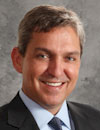
\includegraphics[height=0.1\textheight]{images/rob-enslin.png}}
				& 
				\begin{itemize}
				\item Robert Enslin
				\item Président, opérations client
				\item a rejoint SAP en 1992
				\item a rejoint le conseil d'administration en 2014
				\item le terme de son mandat au conseil expire en 2017
				\item responsabilités particulières : stratégie de marché, cloud, ventes régionales, ventes de l'industrie spécialisée, écosystème, expérience client end-to-end
				\end{itemize}
				\\ 
				
				\raisebox{-\totalheight}{
\includegraphics[height=0.1\textheight]{images/bernd-leukert.png}}
				& 
				\begin{itemize}
				\item Bernd Leukert
				\item produits et innovation
				\item a rejoint SAP en 1994
				\item a rejoint le conseil d'administration en 2014
				\item le terme de son mandat au conseil expire en 2017
				\item responsabilités particulières : organisation du développement global, analyse, application, cloud, bases de données et technologies, mobile
				\end{itemize}
				\\ 
				
				\raisebox{-\totalheight}{
\includegraphics[height=0.1\textheight]{images/lika-mucic.png}}
				& 
				\begin{itemize}
				\item Lika Mucic
				\item Directeur financier, Directeur des opérations
				\item a rejoint SAP en 1996
				\item a rejoint le conseil d'administration en 2014
				\item le terme de son mandat au conseil expire en 2017
				\item responsabilités particulières : finance et administration, relations investisseurs et protection des données
				\end{itemize}
				\\ 
				
				\raisebox{-\totalheight}{
\includegraphics[height=0.1\textheight]{images/oswald.jpg}}
				& 
				\begin{itemize}
				\item Gerhard Oswald
				\item a rejoint SAP en 1981
				\item a rejoint le conseil d'administration en 1996
				\item le terme de son mandat au conseil expire en 2016
				\end{itemize}
				\\ 
				\end{tabular}
		\label{table:board}
	\end{center}
\end{table}
			
\clearpage
			
			

SAP mène une stratégie d'acquisition\footnote{Source : \url{http://www.sap.com/corporate-en/about/investors/newsandreports/acquisitions/index.html}} des leaders des technologies de l'information. La croissance organique étant le moteur de cette stratégie, tout en continuant à investir dans le développement de ses propres produits et dans les technologies innovatrices. Cette stratégie permet à SAP de mieux soutenir l'innovation en la dirigeant vers les partenaires possédant les domaines d'expertise requis. SAP perdure dans ce sens pour acquérir les technologies stratégiques cibles pour couvrir un marché toujours plus grand et pour satisfaire toujours plus les besoins de ses clients.
Le nouveau marché que vise SAP est celui du Big data, dans lequel nous pouvons l'imaginer leader dans quelques années.\\

La structure actuelle est le fruit du rachat de Business Objects par SAP France dont la date l\'{e}gale est le 1er janvier 2010, l'annonce ayant été faite le 7 octobre 2007. Pr\'{e}c\'{e}demment, Business Objects ayant absorb\'{e} deux autres entit\'{e}s, CARTESIS et Crystal decisions. Les rachats de SAP se succèdent : Sybase en 2010, SuccessFactors en 2011, Ariba et Syclo en 2012, Hybris en 2013, FieldGlass et pour finir Concur en 2014.\\







\subsection{Les produits SAP}
Les solutions logicielles de SAP\footnote{Source : \url{http://www.sap.com/france/pc/index.html}} sont principalement à destination des professionnels et offrent un grand nombre de logiciels destiné au traitement de tout type de problématique.\\
Historiquement, SAP est le leader (et inventeur) des progiciels, logiciels de gestion d'entreprise qui ont su, avec le temps, devenir incontournable pour toute moyenne ou grande entreprise.\\
En terme de logiciel de gestion, SAP propose :
\begin{itemize}
	\item Business suite
	\item Développement durable
	\item Gestion comptable et financière
	\item Progiciel de gestion intégré (ERP)
	\item Gestion de la chaine logistique (SCM)
	\item Gestion de la relation client (CRM)
	\item Gestion du cycle de vie des produits (PLM)
	\item Gestion des achats
	\item Gestion des actifs d'entreprise
	\item Gestion des ressources humaines (GRH)
\end{itemize}

Outre le fait de pouvoir organiser les flux d'information de l'entreprise, SAP s'est imposé comme l'un des leaders de l'analyse de ces données.\\
Parmi ces outils d'analyse, nous avons :
\begin{itemize}
	\item Analyse prédictive
	\item Applications analytiques
	\item Business intelligence
	\item Entrepôt de données (Data warehousing)
	\item Gouvernance, risques et conformité
	\item Pilotage de la performance
\end{itemize}

SAP se voulant une entreprise aux solutions complètes et innovantes, elle s'est ouverte aux technologies et aux données. La stratégie d'entreprise de SAP changeant, ainsi que le marché, les domaines de compétences évoluent aussi. Pour illustrer ceci, nous pouvons citer les quelques domaines dans lesquels son expertise est reconnue :

\begin{itemize}
	\item Bases de données
	\item Could computing
	 \item Entrepôt de données
	 \item Gestion de contenu et collaboration
	 \item Gestion de l'information
	 \item Gestion et intégration des processus métier
	 \item Gestion informatique
	 \item Infrastructure / Sécurité des applications métier
	 \item Mobilité
	 \item Platefome de données temps réel (RTDP)
	 \item Technologie In-memory SAP HANA
\end{itemize}

Et pour compléter son large panel de compétences, la stratégie de SAP s'est orientée ces dernières années vers le cloud et vers les technologies mobiles, très à la mode en ce moment. En terme de cloud et de mobilité, nous pouvons citer :
\begin{itemize}
	\item Application métier
	\item Collaboration sociale
	\item Infrastructure
	\item Plate forme
	\item Commerce collaboratif
	\item Applications mobiles
	\item Gestion de flottes de terminaux mobiles
	\item Gestion de mobilité
	\item Plate forme d'applications mobiles
	\item Services mobiles
	\item Solutions de commerce mobile
\end{itemize}

De cet échantillon de solution que propose SAP, nous pouvons être certain de deux choses :
\begin{enumerate}
	\item SAP est le leader et expert des technologies de gestion, de stockage et de traitement des données
	\item Sa stratégie d'expansion et son domaine d'expertise sont orientés vers les systèmes d'information
\end{enumerate}

\subsection{SAP en France}
En France, SAP a implenté des bureaux commerciaux à Lyon, Nantes, Toulouse, Strasbourg, Bordeaux, Aix, Sofia Antipolis et Caen. Leur centre de recherche (SAP Labs) était anciennement à Levallois-Perret (Paris). Paris abritait trois sites SAP différents, ils étaient présents à la défense (principalement pour les ressources humaines), à Capital 8 Paris (principalement pour le développement) et à Levallois-Perret (Développement de solutions et SAP France). Tous ces centres ont été rassemblés en un seul et la fusion s'est terminée mi-avril 2015 quand les locaux de Levallois-Perret front de Seine ont été vidés. Aujourd'hui c'est la tour SAP, à Levallois-Perret, qui accueille les employés des trois sites précédents pour un total de plus de 1600 personnes.

\section{Contexte antérieur à mon arrivée à SAP}

Après le rachat de Business Objects, SAP a sorti la version 4.0 de BOE (Business Objects Entreprise). Le rachat de Business Objects ayant précipité la sortie de BOE, ses fonctionnalités n'étaient pas au rendez-vous, ce qui a grandement déplu les clients. Le logiciel comportait beaucoup de bugs et certaines fonctionnalités n'étaient pas implémentées. 
Ceci s'explique d'une part par le fait que beaucoup trop de fonctionnalités ont été planifiées. Et d'autre part parce que les différentes équipes travaillaient en tunnel, que le trop grand nombre de dépendances rendait très difficile l'intégration complète du produit et que la date de sortie du logiciel ne pouvait pas être repoussée.\\
Mais, gr\^{a}ce aux initiative qualités du groupe Web Intelligence, les versions qui ont suivies ont eu beaucoup de succès. Dans la continuité des initiatives qualité, le groupe Web Intelligence a ainsi amené les huit initiatives qualité.

\subsection{Les 8 initiatives qualité}
\subsubsection{Performance}
\begin{figure}[H]
  \centering
      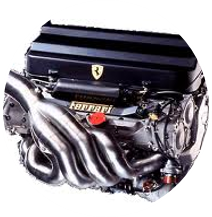
\includegraphics{images/performance.png}
  %\caption{}
	%\label{figure:}
\end{figure}
Améliorer les performances des versions 4.x pour les ramener aux performances de la version 3.1.\\
Les performances critiques étant celles que le client note en premier lieu :
\begin{itemize}
	\item temps d'ouverture d'un document
	\item fonctionnalités de base : création d'un document, sauvegarde, rafra\^{i}chissement
	\item temps de connection au CMS
\end{itemize}


\subsubsection{Intégration continue}
\begin{figure}[H]
  \centering
      
\includegraphics{images/ci.png}
  %\caption{}
	%\label{figure:}
\end{figure}
L'intégration continue doit être assurée de manière à pouvoir détecter le plus tôt possible les régressions (par exemple en compilant ou à chaque livraison de code) et pour pouvoir limiter le risque qu'une compilations casse et de limiter les risques de régressions fonctionnelles en lançant les tests appropriés.\\


\subsubsection{Automatisation}
\begin{figure}[H]
  \centering
      
\includegraphics{images/automation.png}
  %\caption{}
	%\label{figure:}
\end{figure}
Contrôler la qualité de l'héritage inter-versions (compatibilité ascendante) à travers des tests automatiques et assurer la qualité des fonctionnalités en cours de développement.\\
\begin{itemize}
	\item import d'un document créé sur une version 3.x vers une version 4.x
	\item préserver les fonctionnalités et les performances
\end{itemize}

\subsubsection{Optimisation de l'exécution des tests}
\begin{figure}[H]
  \centering
      
\includegraphics{images/produitisation.png}
  %\caption{}
	%\label{figure:}
\end{figure}
Optimiser la couverture de test basée sur les livraisons. \\
Ne pas exécuter les tests qui ne sont pas nécessaires et exécuter ceux qui le sont.

\subsubsection{1 bug = 1 test}
\begin{figure}[H]
  \centering
      
\includegraphics{images/bugtest.png}
  %\caption{}
	%\label{figure:}
\end{figure}
Améliorer la couverture de test de régression en intégrant les anomalies trouvés par les clients dans les fonctionnalités principales. Autrement dit, dès qu'un bug est trouvé un test sera implémenté pour reproduire le problème de manière automatique pour assurer la non-régression. Ce principe permet, comme son nom l'indique, que chacun des bugs corrig\'{e}s par un d\'{e}veloppeur soit test\'{e} syst\'{e}matiquement et automatiquement par un ST\index{Software Tester}.

\subsubsection{Augmenter la couverture de test}
\begin{figure}[H]
  \centering
      
\includegraphics{images/testcoverage.png}
  %\caption{}
	%\label{figure:}
\end{figure}
Trouver les problèmes nouveaux et pas encore découverts en complétant les tests existants, en se concentrant sur les zones à risque.

\subsubsection{ADEPT}
\begin{figure}[H]
  \centering
      
\includegraphics{images/adept.png}
  %\caption{}
	%\label{figure:}
\end{figure}
Réduire le temps de configuration de l'environnement de développement en fournissant des environnement prêts à l'emploi (comprenant IDE, outils de test, codes source, ...) pour toutes les branches BI 4.x.

\subsubsection{Outil de validation des rapports}
\begin{figure}[H]
  \centering
      
\includegraphics{images/validationtool.png}
  %\caption{}
	%\label{figure:}
\end{figure}
Faciliter la migration des clients de la BI4.1 à la BI4.2 en accélérant l'inspection des rapports Web Intelligence après une mise à jour.




%

\chapter{Pr\'{e}sentation de mon environnement \`{a} SAP}


\section{Présentation de l'équipe}




\begin{figure}[h!]
  \centering
      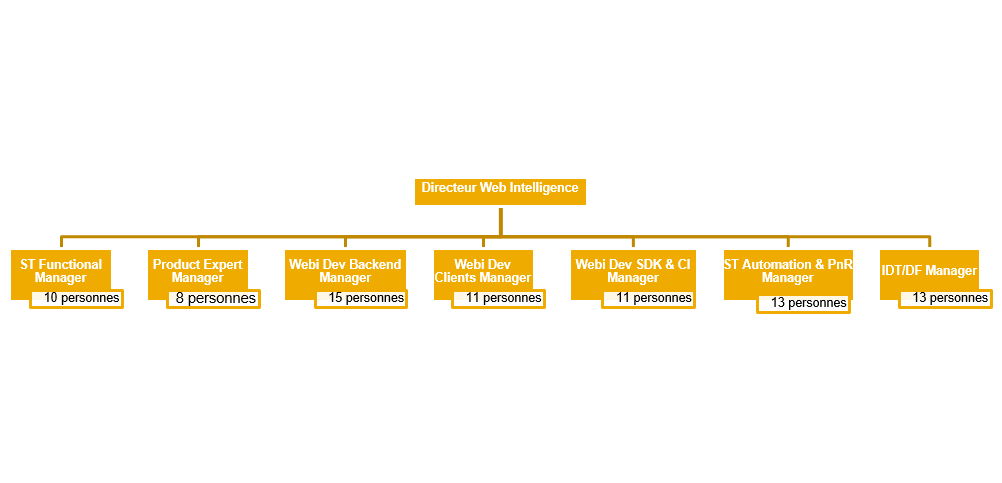
\includegraphics[width=1.2\textwidth]{images/allRaphaelTeam.png}
  \caption{\'{E}quipe Web Intelligence}
	\label{figure:}
\end{figure}








\section{Sa mission}

L'\'{e}quipe transversale fournit les services transversaux, faisant appel à des compétence spécifiques.\\
Particuli\`{e}rement foculis\'{e}e sur le test coverage\index{Test coverage}, différentes missions ce l'\'{e}quipe transverse peuvent être divisées en cinq catégories\footnote{se reporter à l'organigramme page \pageref{pdf:org}} :\\

\begin{description}
	\item[Tests fonctionnels] Assurés par 3 personnes, leurs tests portent sur le SDK de Web Intelligence. 
	\item[Tests automation] Assurés par 3 personnes, leur mission est d'ajouter les tests implémentés et de les mettre en production, quelque soit le test (son Framework ou le langage utilisé).
	\item[Benchmark] Assurés par 3 personnes, ils s'occupent des tests de benchmark, autrement dit, les tests de performance, de stabilité et de scalabilité. Ils sont parfois appelés à implémenter quelques codes mais utilises, en règle général, des logiciels pour générer des charges, ouvrir de multiples documents, installer le produit, répéter la même action des centaines de fois, \ldots. Ils sont aussi en charge des acceptances, autrement dit la validation de tous les tests existants afin de certifier que le produits et fonctionnel.
	\item[Mise en production] Sa mission est de mettre en production les produits développées par et pour les équipes SAP. Une personnes s'occupe de cette mission.
	\item[Développement] Développement d'outils internes et d'outils de reporting, construction de rapport WebI. Une personnes s'occupe de cette mission.
\end{description}








\chapter{Software tester}

%
\section{G\'{e}n\'{e}ralit\'{e}s sur le test automatique}

Pour r\'{e}pondre \`{a} la question \textquote{Qu'est-ce qu'un test automatique?}, je dirais que c'est un code v\'{e}rifiant le bon fonctionnement d'un autre code. Il existe de nombreux niveaux de test : unitaire, fonctionnel, int\'{e}gration, performance, \ldots. Les tests sont tr\`{e}s importants dans un projet logiciel, ils permettent de s'assurer de la conformit\'{e} du logiciel par rapport aux sp\'{e}cifications (autrement dit, le besoin client). La mise en place de ces tests automatiques est facilit\'{e}e par un Framework, il en existe de nombreux mais de mani\`{e}re g\'{e}n\'{e}rale un Framework est un ensemble de librairies et de normes ( de mod\'{e}lisation, d'architecture, ...)\footnote{Source : \url{https://boulaich.wordpress.com/2009/07/08/framework-generalite/}}. \\
\subsection{Description des diff\'{e}rents types de test}

%vas voir ici!!! http://jmdoudoux.developpez.com/cours/developpons/java/chap-frameworks-test.php


\subsubsection{Le test unitaire}
Un test unitaire v\'{e}rifie le bon fonctionnement d'une petite portion de code. En r\`{e}gle g\'{e}n\'{e}rale il s'agit de tester que la valeur retourn\'{e}e par une m\'{e}thode est la bonne, ces tests sont donc impl\'{e}ment\'{e}s par les d\'{e}veloppeurs. Mais il s'agit aussi de valider le fonctionnement de la m\'{e}thode aux limites et de v\'{e}rifier la coh\'{e}rence de ses r\'{e}sultats. Ces tests sont cens\'{e}s \^{e}tre les plus nombreux possibles pour couvrir le maximum de cas possibles, on appelle cela le test coverage (ou couverture de test).

\subsubsection{Le test fonctionnel}
Le test fonctionnel est ax\'{e} sur l'interaction des diff\'{e}rentes m\'{e}thodes, il est ax\'{e} sur les fonctionnalit\'{e}s du logiciel. Ces tests permettent de v\'{e}rifier le bon fonctionnement des sp\'{e}cifications du produit et de valider que les fonctionnalit\'{e}s correspondent aux sp\'{e}cifications. Ceux-ci sont assur\'{e}s par les testeurs automatiques (ST).

\subsubsection{Le test d'int\'{e}gration}
Le test d'int\'{e}gration est au test fonctionnel ce que le test fonctionnel est au test unitaire, avec plusieurs niveaux de granularit\'{e}s (plus ou moins grand nombre de m\'{e}thodes concern\'{e}es). Le test d'int\'{e}gration s'assure du bon fonctionnement du logiciel en interaction avec d'autres logiciels.

\subsubsection{Le test de performance}
Le test de performance s'assure qu'une action est effectu\'{e}e dans le temps imparti. Les actions test\'{e}es sont aux minimum celles qui composent les workflows nominaux, tant s\'{e}par\'{e}ment que simultan\'{e}ment (multi utilisateurs).

\subsubsection{Le test de stabilit\'{e}}
Le test de stabilit\'{e} permet de tester qu'un comportement est syst\'{e}matique, autrement dit qu'une m\^{e}me action implique toujours le m\^{e}me r\'{e}sultat.\\
Les tests de stabilit\'{e}s permet de s'assurer que la r\'{e}ponse est bien l\`{a} dans le temps imparti et qu'il n'y a pas d'erreurs, ceci en faisant subir une mont\'{e}e en charge des requ\^{e}tes du logiciel sur une dur\'{e}e pouvant aller de 24 \`{a} 72 heures.

\subsubsection{Le test de scalabilit\'{e}}
Le test de scalabilit\'{e} permet de s'assurer que le logiciel peut \'{e}voluer de mani\`{e}re \`{a} pouvoir offrir les m\^{e}mes performances dans un contexte d'utilisation qui a \'{e}volu\'{e}. Par exemple, dans le cas o\`{u} la charge d'utilisation double, est-il possible de modifier l'environnement client afin que les utilisateurs profitent des m\^{e}mes performances?


\subsubsection{Le test de validation de plateforme}
Ce type de test est consacr\'{e} aux logiciels destin\'{e}s \`{a} \^{e}tre utilis\'{e}s sur plusieurs plateformes. D'un syst\`{e}me d'exploitation \`{a} un autre, les comportements sont-ils les m\^{e}mes? Les fonctionnalit\'{e}s sont-elles identiques?

\section{Le test dans l'\'{e}quipe d'automatisation des tests}
Lorsque je suis arriv\'{e} dans cette \'{e}quipe, j'ai d\'{e}couvert des logiciels que je ne connaissais pas : Perforce, ASTEC, Jenkins, et d'autres. J'ai mis un peu de temps \`{a} me les approprier et \`{a} bien comprendre \`{a} quoi ils servaient exactement. La complexit\'{e} de leur environnement d'utilisation ne m'a pas facilit\'{e} la t\^{a}che. 

Pour r\'{e}sumer ce que j'ai appris sur les g\'{e}n\'{e}ralit\'{e}s de cette \'{e}quipe c'est qu'elle utilise plusieurs outils pour g\'{e}rer le code des diff\'{e}rents logiciels, poss\'{e}dant chacun plusieurs versions. Pour chacune de ces versions une suite de tests est ex\'{e}cut\'{e}e quotidiennement, les codes en question sont h\'{e}berg\'{e}s sur le gestionnaire de code source Perforce\index{Perforce}. 

Apr\`{e}s chaque livraison de code effectu\'{e}e, le logiciel est compil\'{e} par Jenkins. Et, de plus, le logiciel est compil\'{e} quotidiennement par ASTEC dont les r\'{e}sultats sont automatiquement envoy\'{e}s aux personnes concern\'{e}es (cf. annexe \ref{pdf:automationResults} page \pageref{pdf:automationResults} qui pr\'{e}sente l'un des r\'{e}sultats de ces mails). L'utilisation de ASTEC dans l'\'{e}quipe est beaucoup plus large que cela mais je n'ai pas eu l'occasion de l'\'{e}tudier plus en d\'{e}tail.\\



Le testeur automatique est focalis\'{e} sur les fonctionnalit\'{e}s du logiciel. Lorsque les sp\'{e}cifications d'une nouvelle fonctionnalit\'{e} voient le jour, un plan de test est r\'{e}dig\'{e} et est envoy\'{e} \`{a} l'\'{e}quipe du test automatique. Du test plan sont extraits tous les tests pouvant \^{e}tre automatis\'{e}s et ceux-ci sont impl\'{e}ment\'{e}s.\\
Je n'ai pas beaucoup particip\'{e} \`{a} cet aspect de l'\'{e}quipe, ma principale mission relevait de l'initiative \textquote{1 bug - 1 test}. Mon travail n'\'{e}tait pas de tester une nouvelle fonctionnalit\'{e} mais plut\^{o}t, une fonctionnalit\'{e} d\'{e}j\`{a} existante sur laquelle une anomalie a \'{e}t\'{e} trouv\'{e}e, soit par un client (\`{a} \'{e}viter) soit par un individu interne \`{a} SAP.\\

Le cycle de d\'{e}veloppement de l'automatisation de tests dans lequel j'ai \'{e}volu\'{e} est r\'{e}sum\'{e} (et simplifi\'{e}) figure \ref{figure:testProcess} page \pageref{figure:testProcess}. Ce cycle est celui de l'automatisation d'un test dans le cas d'une anomalie trouv\'{e}e sur une fonctionnalit\'{e} existante et pas sur une nouvelle fonctionnali\'{e}. Mon int\'{e}gration dans ce processus de d\'{e}veloppement m'a appris beaucoup, non seulement quant \`{a} la gestion d'une anomalie logicielle, mais surtout quant \`{a} la valeur et \`{a} l'utilisation du test qui peut \^{e}tre impl\'{e}menté soit en r\'{e}ponse \`{a} une anomalie soit dans le processus initial de d\'{e}veloppement pour garantir qu'une fonctionnalit\'{e} se comporte telle qu'elle est d\'{e}crite dans les sp\'{e}cifications.\\
\begin{figure}[!ht]
  \centering
      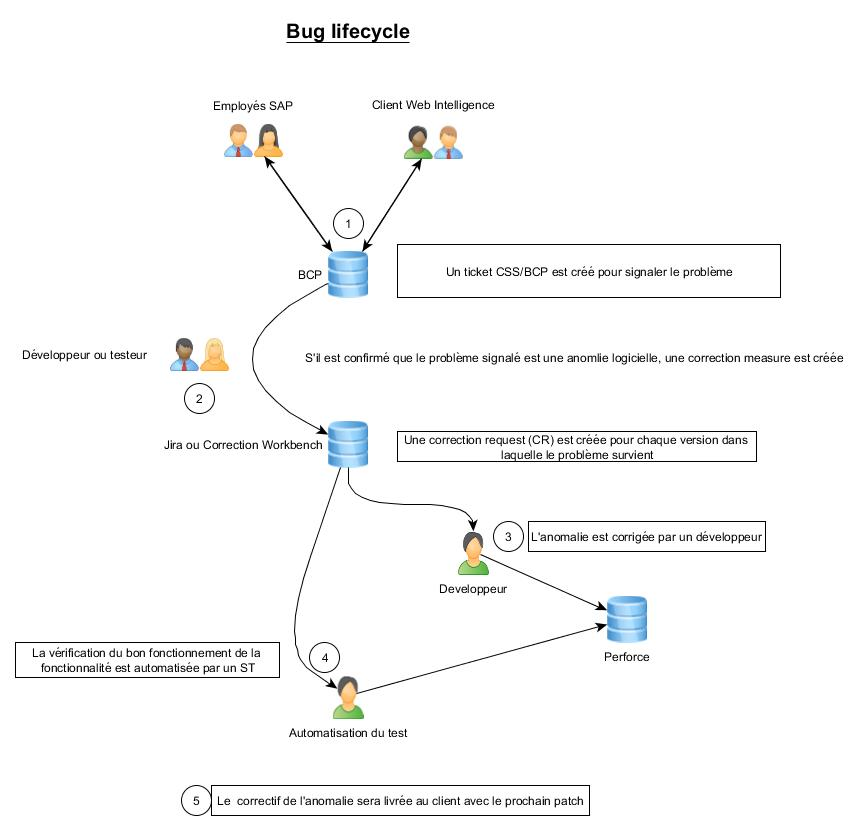
\includegraphics[width=\textwidth]{images/testProcessAtSAP.jpg}
  \caption{Le process de test}
	\label{figure:testProcess}
\end{figure}
 


\section{Pr\'{e}sentation du produit test\'{e} : Web Intelligence}
Web Intelligence est un logiciel de BI\index{Business Intelligence} permettant d'acc\'{e}der \`{a} des donn\'{e}es stock\'{e}es dans une base de donn\'{e}es. Cet acc\`{e}s aux donn\'{e}es ne se fait pas directement, tout l'int\'{e}r\^{e}t de Web Intelligence repose sur l'utilisation d'une couche s\'{e}mantique, \textquote{l'univers}.\\
Il existe trois interfaces graphiques permettant d'acc\'{e}der \`{a} ces donn\'{e}es, un client lourd et deux clients l\'{e}gers : l'applet et le client dhtml.



\section{La premi\`{e}re semaine dans l'\'{e}quipe d'automatisation des tests}
\`{A} mon arriv\'{e}e dans l'\'{e}quipe et avant de commencer \`{a} impl\'{e}menter des tests automatiques, j'ai \'{e}t\'{e} accueilli par mes coll\`{e}gues et on m'a fourni le mat\'{e}riel n\'{e}cessaire au bon d\'{e}roulement de mon travail.\\
Mes 1\up{er} jours \`{a} SAP se sont d\'{e}roul\'{e}s de la mani\`{e}re suivante :\\
\begin{itemize}
\item Pr\'{e}sentation \`{a} l'\'{e}quipe et visite des locaux
\item R\'{e}union avec mon tuteur et mon manager pour une description de la mission
\item R\'{e}cup\'{e}ration des diff\'{e}rents droits d'acc\`{e}s aux serveurs
\item Familiarisation avec les outils internes (tickets HR, CSS, IT, ...)
\item Installation des logiciels n\'{e}cessaires au d\'{e}veloppement (IDE, SCM\index{Source Code Management}, \'{e}diteur de texte, \ldots)
\item Mise en place du framework de test (cr\'{e}ation du workspace perforce)
\end{itemize}
Au terme de la 1\up{\`{e}re} semaine, j'ai pu commencer \`{a} \'{e}tudier le framework de test en me basant sur les tests d\'{e}j\`{a} existants.\\
C'est au cours de la deuxi\`{e}me semaine que j'ai pu impl\'{e}menter mes 1\up{er} tests.


%\glspl{pois} \\
%\glspl{vache} \\
%\glspl{pigeon} \\
% \glspl{TEM}  \\
% \gls{latex}  \\
%\glspl{lvm}








\section{Travail r\'{e}alis\'{e}}

Tout au long de cette mission, ou plut\^{o}t ces missions (un test achev\'{e} laisse toujours la place \`{a} un autre), j'ai travaill\'{e} \`{a} impl\'{e}menter des tests en Java permettant de valider automatiquement le comportement de WebI au niveau SDK.

L'objectif principal de cette mission \'{e}tait d'\^{e}tre, \`{a} terme, capable d'impl\'{e}menter seul et dans les plus brefs d\'{e}lais un test automatique. La grande difficult\'{e} de d\'{e}but de cette mission a \'{e}t\'{e} de comprendre, d'une part, la logique du framework\index{Framework} de test, et d'autre part les diff\'{e}rentes choses que celui-ci me permettait de faire.\\

Les concepts \`{a} assimiler \'{e}taient nombreux et j'ai pass\'{e} beaucoup de temps \`{a} essayer de comprendre le Framework sur lequel repose l'impl\'{e}mentation des tests. Les probl\`{e}mes majeurs que j'ai rencontr\'{e}s au d\'{e}but sont les diff\'{e}rents points suivants :
\begin{itemize}
	\item Comment int\'{e}grer un test \`{a} l'ensemble des tests ex\'{e}cut\'{e}s?
  \item Quel type de test mettre en place, statique ou dynamique?
	\item Comment initialiser un test?
	\item Comment g\'{e}rer les sources de telle ou telle version du logiciel pour impl\'{e}menter un test automatique?
	\item O\`{u} trouver les fichiers de r\'{e}f\'{e}rences n\'{e}cessaires?
\end{itemize}

J'ai \'{e}clairci tous ces points au fur et \`{a} mesure de mes missions et de mes exp\'{e}rimentations. Certains sont tr\`{e}s simples \`{a} assimiler mais d'autres m'ont pos\'{e}s beaucoup de probl\`{e}mes. Je d\'{e}taille dans les parties suivantes comment est-ce que j'ai \'{e}t\'{e} confront\'{e} \`{a} ces diff\'{e}rents probl\`{e}mes et la mani\`{e}re dont je m'y suis pris pour les r\'{e}soudre. Dans la partie qui suit je pr\'{e}senterai les diff\'{e}rents probl\`{e}mes que j'ai rencontr\'{e} et la mani\`{e}re dont je m'y suis pris pour les r\'{e}soudre. Dans le souci de rester clair dans mes explications je ne m'\'{e}parpillerai pas sur tous les tests que j'ai impl\'{e}ment\'{e} qui m'ont mis face \`{a} tel ou tel probl\`{e}me. Je partirai plut\^{o}t d'un cas simple de test automatique en consid\'{e}rant que tous ces probl\`{e}mes se sont succ\'{e}d\'{e}s dans le cadre du m\^{e}me test.\\


\subsection{Les recherches relatives aux tests automatiques dans le cadre du Framework utilis\'{e}}


Ne connaissant rien ni de Web Intelligence ni du Framework de test, je me suis d'abord pench\'{e} la mani\`{e}re d'utiliser ce Framework pour impl\'{e}menter un code simple manipulant un document Web Inteliigence.\\

Pour se faire, j'ai choisi une fonctionnalit\'{e} tr\`{e}s simple, le d\'{e}placement d'une cellule dans un tableau, me basant sur un document de test mis \`{a} ma disposition (illustration de ce document figure \pageref{figure:docsample}).\\

\begin{figure}[!h]
  \centering
      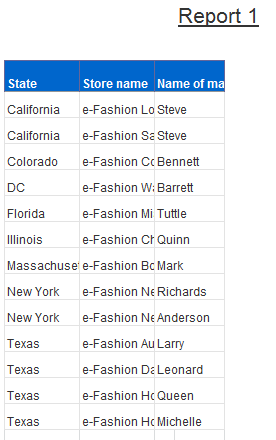
\includegraphics{images/docsample.png}
  \caption{Document sur lequel j'ai bas\'{e} mes premi\`{e}re exp\'{e}rimentations}
	\label{figure:docsample}
\end{figure}
 
Partant de ce document, comment devais-je m'y prendre pour automatiser une action sur celui-ci? Pour se faire il me fallait me baser sur une impl\'{e}mentation de test automatique d\'{e}j\`{a} exitante. J'ai donc chercher un code dont la structure me permettait de manipuler un document Web Intelligence d\'{e}j\`{a} existant. Il en existe beaucoup de types diff\'{e}rents mais j'ai rapidement trouv\'{e} l'exemple d'un test qui se basait sur un document Web Intelligence. J'ai donc cr\'{e}\'{e} une nouvelle \gls{Classe} pour mon test et ai coll\'{e} le code \'{e}pur\'{e} \`{a} l'int\'{e}rieur, j'avais donc une \gls{Classe} Java me permettant d'effectuer un test sur mon document. Mais \`{a} cette \'{e}tape j'ai rencontr\'{e} un certain nombre de probl\`{e}mes m'emp\^{e}chant de tester mon code qui ne compilait pas.\\
J'ai pass\'{e} beaucoup de temps \`{a} chercher les solutions dans les messages d'erreurs que je re\c{c}evais en masse.\\

J'avais pris le soin de coller mon document Web Intelligence pr\'{e}cis\'{e}ment dans le dossier qu'il fallait mais pourtant, les messages d'erreur me disait que le document \'{e}tait introuvable. En investiguant tous les documents rentrant en jeu dans l'ex\'{e}cution du test et en r\'{e}fl\'{e}chissant \`{a} la signification de chacune des variables, je me suis rendu compte que je n'avais pas modifi\'{e} le \textquote{script ID} du fichier script.xml. Celui-ci permet d'identifier un plan de test, qui lui-m\^{e}me identifie une ou plusieurs \gls{Classe}s de test. Une fois la modification effectu\'{e}e, en prenant soin de correctement renseigner le nom de mon test, je suis tomb\'{e} une fois de plus sur une erreur similaire : le document demeure introuvable. Le plan de test \'{e}tant ex\'{e}cut\'{e}, cette fois-ci, l'erreur ne pouvait se trouver que dans ma \gls{Classe} de test. J'ai rapidement identifi\'{e} le probl\`{e}me puisque c'est dans cette m\^{e}me \gls{Classe} que le chemin d'acc\`{e}s \`{a} mon fichier est renseign\'{e}. Les r\'{e}pertoires \'{e}tant nomm\'{e}s diff\'{e}remment en fonction de la suite de test \`{a} laquelle ils appartiennent, et, le test que je voulais ex\'{e}cuter ne faisant pas partie de la m\^{e}me suite, lors de l'ex\'{e}cution Java n'allais pas chercher mon document dans le bon r\'{e}pertoire. J'ai donc corrig\'{e} cette erreur et ai renseign\'{e} la bonne valeur.\\
En ex\'{e}cutant de nouveau, je constate qu'il n'y a plus de probl\`{e}mes d'acc\`{e}s \`{a} un fichier. Cette fois-ci les messages d'erreur m'annoncent qu'il est impossible d'acc\'{e}der au \gls{CMS}. Je me dirige donc vers le \gls{CMS} en question pour r\'{e}cup\'{e}rer son adresse puis vers le fichier parameters.xml dans lequel l'url du \gls{CMS} est renseign\'{e}e, effectivement ce n'\'{e}tait pas la m\^{e}me, mais d'autre part en essayant d'acc\'{e}der au \gls{CMS} dont il \'{e}tait question je constatais que celui-ci n'existait plus, je ne pouvais pas y acc\'{e}der. J'ai donc corrig\'{e} l'adresse du \gls{CMS} sur lequel je voulais faire mon test.\\
En ex\'{e}cutant une fois de plus j'ai \'{e}t\'{e} ravi de voir que mon test compilais, celui-ci ne faisait encore rien mais je pouvais alors commencer \`{a} manipuler mon document Web Intelligence en impl\'{e}mentant le code de mon test automatique.\\

La question qui se posa alors \'{e}tait de savoir comment y acc\'{e}der et de quelle mani\`{e}re m'y prendre pour le modifier.\\
En parcourant les tests automatiques existants et en cherchant les informations qui me manquaient, j'ai constat\'{e} avec surprise que nul part dans le code il n'y avait de commentaires pour expliquer la d\'{e}marche utilis\'{e}e ou la logique appliqu\'{e}e. Ce qui m'a troubl\'{e}, puisque l'on m'avais toujours enseign\'{e} que les commentaires sont essentiels dans toute impl\'{e}mentation. J'ai \'{e}videmment pos\'{e} la question pour en connaitre la raison. Les \'{e}quipes de d\'{e}veloppement et de test de Web Intelligence travaillant en suivant la m\'{e}thode agile, celles-ci sont cens\'{e}es \'{e}crire des codes clairs au point que le code lui-m\^{e}me suffit \`{a} sa compr\'{e}hension. Les quelques rares commentaires servant \`{a} expliquer le fonctionnement g\'{e}n\'{e}ral d'une grande portion de code. Je comprenais ce principe mais j'\'{e}tais d\'{e}rang\'{e} par le fait que chacun des objets utilis\'{e}s dans le code m'\'{e}taient inconnus, ce qui augmentait beaucoup le temps qu'il me fallait pour comprendre une certaine impl\'{e}mentation.\\ 

En cherchant parmi les tests automatiques existants j'ai trouv\'{e} le code qui me permettrait de r\'{e}cup\'{e}rer mon document :
\begin{lstlisting}
IRSReport monRapport = docCalc.getReportAurora(0);
\end{lstlisting}

L'objet \textquote{docCalc} appartenant \`{a} la super \gls{Classe} de ma \gls{Classe} de test, contient un grand nombre de m\'{e}thodes permettant de manipuler un document Web Intelligence. L'argument \textquote{0} que je passe \`{a} la m\'{e}thode me permet de r\'{e}cup\'{e}rer le premier rapport que contient mon document. Pour compl\'{e}ter ce code ci-dessus et le faire ressembler \`{a} test il faut marquer le d\'{e}but et la fin du test. Le code compl\'{e}t\'{e} \'{e}tant le suivant :


\begin{lstlisting}
IRSReport reportAurora = docCalc.getReportAurora(0);
startTestcaseStep("monTest");
stopTestcaseStepWithAction();
\end{lstlisting}
 
En observant les logs de l'ex\'{e}cution de ce test, on remaque que la premi\`{e}re m\'{e}thode \textquote{startTestcaseStep("");} permet de marquer le d\'{e}but des tests, celle-ci ne fait rien d'autre que d'ajouter un log. Ensuite, \textquote{stopTestcaseStepWithAction();} marque non seulement la fin du test dans les logs mais aussi ex\'{e}cute une s\'{e}rie d'actions qui sont d\'{e}critent dans les logs. Il est int\'{e}ressant de les noter ici car ces actions peuvent nous \^{e}tre tr\`{e}s utiles.\\
L'\'{e}tude des ces logs m'a \'{e}t\'{e} d'une grande aide car ceux-ci d\'{e}crivent pr\'{e}cis\'{e}ment l'ex\'{e}cution du test.\\




\subsubsection{Recherche effectu\'{e}es pour conna\^{i}tre les diff\'{e}rentes actions de l'ex\'{e}cution d'un test}
Les logs sont nombreux et j'ai pass\'{e} beaucoup de temps \`{a} les analyser. J'ai pu en conclure les trois \'{e}tapes essentielles, et \'{e}videntes, de l'ex\'{e}cution d'un test : l'avant test, le pendant et l'apr\`{e}s. Un exemple d'une de ces sorties consoles que j'ai ainsi \'{e}tudi\'{e} est disponible annexe \ref{annexe:sortieConsole} page \pageref{annexe:sortieConsole} dans laquelle j'ai distingu\'{e} les diff\'{e}rentes parties depuis lesquelles les logs \'{e}taient g\'{e}n\'{e}r\'{e}s.\\
Pour faire ces obsvervations j'ai simplement ajout\'{e} des logs au moments cl\'{e}s de l'ex\'{e}cution : au d\'{e}but et \`{a} la fin du constructeur et de mon test (en distinguant la m\'{e}thode de test et l'impl\'{e}mentation du test). Cela m'a permis d'observer et ainsi de comprendre les diff\'{e}rentes \'{e}tapes du test tels qu'ils \'{e}taient dans le Framework que j'utilisais. Les tests que j'impl\'{e}mentais \'{e}taient ex\'{e}cut\'{e}s dans un cycle propre au Framework, cycle qui m'\'{e}tait inconnu et sans documentation. De cette mani\`{e}re j'ai pu, d'une part, observer dans quelle ex\'{e}cution s'inscrivait mon test, d'autre part, \'{e}tudier l'ex\'{e}cution de mon test lui-m\^{e}me et comprendre l'utilit\'{e} de certaines fonctions. Ci-dessous la liste d\'{e}scriptive de ce que j'ai pu d\'{e}duire de cette \'{e}tude (la m\'{e}thode \textquote{run()} dont je parle et la m\'{e}thode contenant l'impl\'{e}mentation de mon test automatique) :

\begin{enumerate}
	\item Avant la m\'{e}thode \textquote{run()}
	\begin{itemize}
		\item Avant toute chose, ce sont les informations contenues dans le fichier parameters.xml qui sont r\'{e}cup\'{e}r\'{e}es, autrement dit, le \gls{CMS} sur lequel le test devra \^{e}tre effectu\'{e}
		\item V\'{e}rifie l'existence du dossier contenant les ressources utilis\'{e}s dans le cadre de tout test
		\item Cr\'{e}ation du fichier dans lequel seront enregistr\'{e}s les logs 
		\item Connexion au serveur (CSM)
		\item Recherche le dossier FavoritesFolder sur le \gls{CMS}
		\item Supprime, en local, les dossier o\`{u} sont enregistr\'{e}s les r\'{e}sultats (\textbackslash res\textbackslash  et \textbackslash ref\textbackslash )
		
	\end{itemize}
	\item Pendant la m\'{e}thode \textquote{run()} et avant la m\'{e}thode \textquote{stopTestcaseStepWithAction();}
	\begin{itemize}
		\item Recherche de l'univers mentionn\'{e} dans l'impl\'{e}mentation du test automatique
		\item Cr\'{e}ation d'un nouveau document sur les \gls{CMS}, celui-ci est suivi du nom que j'ai donn\'{e} \`{a} l'ex\'{e}cution de mon test (\textquote{startTestcaseStep("monTest");}) de telle sorte que je vais retrouv\'{e} sur le \gls{CMS} le document que j'avais en local.
	\end{itemize}
	\item Pendant la m\'{e}thode \textquote{stopTestcaseStepWithAction();} (cette m\'{e}thode \'{e}tant comprise dans la m\'{e}thode \textquote{run()})
	\begin{itemize}
		\item Cr\'{e}ation du dossier o\`{u} les r\'{e}sultats seront enregistr\'{e}s
		\item Recherche le dossier \textquote{Personnal Documents} sur le \gls{CMS}
		\item Recherche sur le \gls{CMS} du document concern\'{e} par mon test (ce document se retrouve en deux endroits et dans deux \'{e}tats diff\'{e}rents, sur le \gls{CMS} et en local, avant test et apr\`{e}s test)
		\item Sauvegarde du document en local
		
	\end{itemize}
	\item Apr\`{e}s la m\'{e}thode \textquote{run()}
	\begin{itemize}
		\item Sauvegarde du document dans le personal folder du \gls{CMS}
		\item Copie la r\'{e}f\'{e}rence du cube (r\'{e}f\'{e}rence que j'ai moi-m\^{e}me d\'{e}pos\'{e}) vers le dossier \textbackslash ref\textbackslash
		\item Cr\'{e}e le dossier qui recevra les r\'{e}f\'{e}rences
		\item Compare le document cr\'{e}\'{e} avec la r\'{e}f\'{e}rence
	\end{itemize}
\end{enumerate}

Durant cette partie de mon travail, o\`{u} l'investigation c'est \'{e}tal\'{e}e sur plusieurs semaines et portant sur plusieurs tests \`{a} impl\'{e}menter, j'ai d\'{e}couvert \'{e}norm\'{e}ment de choses aussi bien en Java que sur l'utilisation du Framework de test. J'ai pu mettre au point des m\'{e}thodes de r\'{e}solution de mes probl\`{e}mes et ai pu d\'{e}couvrir la majeure partie des objets utilis\'{e}s lors de l'impl\'{e}mentation des tests automatiques de Web Intelligence.


\subsubsection{Manipulation des diff\'{e}rents objets du Framework}

Ayant maintenant \'{e}tudi\'{e} toute l'ex\'{e}cution du test, je suis plus \`{a} m\^{e}me de situer le test automatique dans sa globalit\'{e}.\\
La question qui se pose maintenant est de savoir quoi mettre dans le test, avant de pouvoir se poser la vraie question : \textquote{Comment tester automatiquement une fonctionnalit\'{e}?}. Au d\'{e}but, je consid\'{e}rai que toute modification applicable depuis l'interface graphique pouvait \^{e}tre reproduite depuis le test. J'avais tord. Mes tests automatiques \'{e}tant des tests au niveau SDK, les fonctionnalit\'{e}s auxquelles j'avais acc\`{e}s et que je pouvais tester \'{e}taient donc limit\'{e}es \`{a} celui-ci.\\

Pour en revenir \`{a} l'impl\'{e}mentation de mon test de base, devant d\'{e}placer une cellule, la mani\`{e}re la plus simlple \'{e}tait de trouver quelque part dans les tests existants comment cette fonctionnalit\'{e} \'{e}tait utilis\'{e}e. Je n'ai pas trouv\'{e} d'exemple me permettant d'appliquer rapidement ce changement \`{a} mon document mais j'ai trouv\'{e} des pistes qui para\^{i}ssaient prometteuses. La recherche du mot \textquote{drop} dans le Framework m'a retourn\'{e} beaucoup de r\'{e}sultats dont un qui a retenu mon attention, il existe un objet \textquote{DropHelperImpl}. On en d\'{e}duit assez facilement, \`{a} partir de son nom, que celui \`{a} quelque chose \`{a} voir avec le d\'{e}placement d'une cellule. Il me fallait trouver un exemple d'utilisation de cet objet pour faciliter mon travail, fort heureusement il existe une fonctionnalit\'{e} d'\gls{Eclipse} que je ne connaissais pas avant (et que, depuis lors, je me suis mis \`{a} utiliser syst\'{e}matiquement) : \textquote{get call heirarchy}, me permettant d'avoir le d\'{e}tail de tous les emplacements o\`{u} cette \gls{Classe} est instanci\'{e}e. De cette mani\`{e}re j'ai rapidement trouv\'{e} des exemple de codes me permettant d'en d\'{e}duire les quelques informations qui m'\'{e}taient n\'{e}cessaires.\\

J'ai comprise que je ne pouvais pas faire ce que je voulais directement, il me fallait pr\'{e}parer le terrain et r\'{e}cup\'{e}rer tous les objets qui entraient en jeu dans le d\'{e}placement de la cellule.\\

Il fallait d'abord r\'{e}cup\'{e}rer, \'{e}videmment, le corps de mon document, cela se fait simplement gr\^{a}ce \`{a} l'une des \gls{M\'{e}thode}s propres au rapport :
\begin{lstlisting}
reportAurora.getPageZone(PageZoneType.BODY);
\end{lstlisting}
L'\'{e}tape suivante \'{e}tait de r\'{e}cup\'{e}rer le tableau contenu dans le corps du document, le probl\`{e}me \'{e}tant que pour se faire il faut appeler l'objet par son nom. Comment savoir comment ce tableau a \'{e}t\'{e} appel\'{e}? Car je pouvais acc\'{e}der \`{a} mon document depuis Web Intelligence mais, depuis l'interface, je n'avais aucun moyen de savoir ce qui se passait derri\`{e}re, c\^{o}t\'{e} logiciel.\\
La m\'{e}thode que j'ai utilis\'{e} \`{a} ce moment l\`{a} et que j'ai toujours continu\'{e} \`{a} utiliser \'{e}tait de parcourir l'ensemble des \'{e}l\'{e}ments contenu dans le corps du rapport et d'en afficher les propri\'{e}t\'{e}s. Cela me permettais, non seulement, d'obtenir son nom, son identifiant et tout ses param\`{e}tres, mais aussi, d'obtenir son type. Au fur est \`{a} mesure du temps et que j'impl\'{e}mentais des tests j'ai d\'{e}couvert beaucoup de types diff\'{e}rents, leurs imbriquations, utilit\'{e}s et correspondances avec les \'{e}l\'{e}ments graphiques du document Web Intelligence.\\
Gr\^{a}ce \`{a} cette m\'{e}thode, j'ai pu d\'{e}terminer le nom de ce que je cherchais.\\
Ensuite, de cette table il me fallait r\'{e}cup\'{e}rer les colonnes, pour pouvoir les manipuler. Dans les diff\'{e}rents tests que j'avais pu \'{e}tudier auparavant, j'avais remarqu\'{e} l'utilisation d'une \gls{M\'{e}thode} g\'{e}n\'{e}rique permettant de r\'{e}cup\'{e}rer une cellule d'un tableau. J'ai utilis\'{e} cette \gls{M\'{e}thode} de la m\^{e}me mani\`{e}re que celle utilis\'{e}e dans les tests existants. \\
Alors j'ai pu impl\'{e}menter le code suivant qui me permettait de d\'{e}placer une colonne :


\begin{lstlisting}
IRSPageZone pageZone = reportAurora.getPageZone(PageZoneType.BODY);
IRSReportElement findReportElement = docCalc.findReportElement(pageZone.getChildren(), "Block 1");
IRSDynamicBlock table = (IRSDynamicBlock) findReportElement;
IRSCell cell1 = docCalc.getCellFromTable("State",(IRSTable) table);
IRSCell cell2 = docCalc.getCellFromTable("Store name ",(IRSTable) table);
IRSCell cell3 = docCalc.getCellFromTable("Name of manager ",(IRSTable) table);

DropHelperImpl dropHelp = new DropHelperImpl();
List<IRSCell> cells = new ArrayList<IRSCell>();
cells.add(cell1);
cells.add(cell2);
dropHelp.dropCells(cells, cell3, CellZone.RIGHT);
docCalc.applyFormat();
\end{lstlisting}

L'utilisation de la \gls{M\'{e}thode} \textquote{dropCells()} n'est pas instinctive, au premier abord, et j'ai fais plusieurs essais avant de comprendre son fonctionnement. Cette \gls{M\'{e}thode} prends trois param\`{e}tres : un tableau de cellules, une cellule et une position. Le changement appliqu\'{e} par cette \gls{M\'{e}thode} est que le contenu du tableau de cellule est d\'{e}plac\'{e} comme d\'{e}sir\'{e}, ici, \`{a} droite de la cellule sp\'{e}cifi\'{e}e.\\
La modification appliqu\'{e}e par ce code est illustr\'{e}e figure \ref{figure:dropcells}.\\

\begin{figure}[!h]
  \centering
      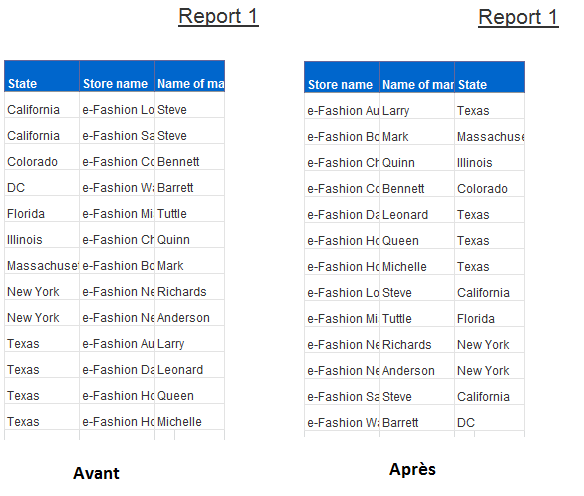
\includegraphics{images/dropcells.png}
  \caption{Allure du tableau avant et apr�s l'ex\'{e}cution du code}
	\label{figure:dropcells}
\end{figure}


\subsection{}












%

\section{Synth\`{e}se des connaissances}
Dans cette partie, je d\'{e}taille l'ensemble des connaissances que j'ai accumul\'{e} sur l'impl\'{e}mentation d'un test automatique d'une fonctionnalit\'{e} de Web Intelligence.\\

\subsection{Tests statiques ou dynamiques}

Le test, qu'il soit statique ou dynamique, sera ex\'{e}cut\'{e} avec tous les autres d\`{e}s lors que le nom du test plan est inscrit dans la \gls{Testsuite}\index{Testsuite}.\\
La diff\'{e}rence fonctionnelle entre ces deux types de tests est que l'un ne fait que comparer deux documents Web Intelligence alors que l'autre permet d'appliquer un certain nombre des modifications sans pour autant les comparer syst\'{e}matiquement \`{a} la fin.\\
La diff\'{e}rence en terme de consommation de temps est tr\`{e}s importante, puisque pour un test statique il n'est pas n\'{e}cessaire d'\'{e}crire le code du \gls{Testcase}\index{Testcase}! Voyons ceci plus en d\'{e}tail.

\subsubsection{Tests statiques}
Globalement, le test statique :

\begin{itemize}
	\item compare un document par rapport \`{a} une r\'{e}f\'{e}rence
	\item demande peu de connaissances techniques, que ce soit en \gls{Java} ou sur Web Intelligence
\end{itemize}

La question \`{a} se poser est : \textquote{Quand impl\'{e}menter un test statique?}.\\
Je n'en ai impl\'{e}menter que quelques-uns, l'int\'{e}r\^{e}t en terme de difficult\'{e} et de choses \`{a} apprendre, \'{e}tant limit\'{e}. Mais je pense pouvoir dire qu'un test de ce type n'est utilis\'{e} que pour valider que l'ouverture d'un document se fait correctement. Autrement dit, ce test permet de s'assurer des compatibilit\'{e}s ascendantes de Web Intelligence.\\

\textbf{Principe du test statique}\hfill \\ \indent
Lors de l'ex\'{e}cution d'un test statique, un fichier est g\'{e}n\'{e}r\'{e} \`{a} partir d'un fichier puis, celui-ci est compar\'{e} avec un fichier de r\'{e}f\'{e}rence.\\
Si les deux fichiers sont identiques, le test est correct, sinon il \'{e}choue.\\
Au fur est \`{a} mesure de mes tests j'ai pu d\'{e}duire ce que devait contenir n\'{e}cessairement les diff\'{e}rents fichiers \`{a} impl\'{e}menter et les relations qu'ils entretenaient entre eux.\\
Pour l'ex\'{e}cution d'un test statique, il faut impl\'{e}menter un \gls{Testplan} qui respecte la structure suivante :

\lstinputlisting[language=java]{scripts/basicStaticTest.java}

J'ai \'{e}t\'{e} \'{e}tonn\'{e}, la premi\`{e}re fois que j'ai compiler un test de ce type, de le voir \'{e}chouer. Ce que j'ai rapidement compris car son r\^{o}le est de comparer le fichier r\'{e}sultant de ce test avec une r\'{e}f\'{e}rence, r\'{e}f\'{e}rence qui n'existe pas. Le probl\`{e}me auquel j'ai \'{e}t\'{e} confront\'{e} \'{e}tait de savoir comment g\'{e}n\'{e}rer cette r\'{e}f\'{e}rence. J'avais d\'{e}j\`{a} remarqu\'{e} que, gr\^{a}ce \`{a} une configuration particuli\`{e}re du fichier script.xml (voir figure \ref{figure:scriptXmlSavingRef} page \pageref{figure:scriptXmlSavingRef}), des fichiers \'{e}taient g\'{e}n\'{e}r\'{e}s lors de l'ex\'{e}cution de mes tests. Je me suis alors rendu dans le r\'{e}pertoire o\`{u} ces fichiers se trouvaient et ai copier celui-ci dans le dossier des r\'{e}f\'{e}rences. Ceci fait le test n'\'{e}chouait plus, mais comment savoir si ce fichier de r\'{e}f\'{e}rence est fiable? Le r\^{o}le du \gls{Software tester} est de s'assurer que ce fichier peut-\^{e}tre utlis\'{e} comme r\'{e}f\'{e}rence.\\

\begin{figure}[!ht]
  \centering
      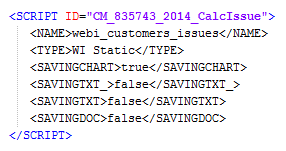
\includegraphics{images/scriptXmlSavingRef.png}
  \caption{Contenu du script.xml pour g\'{e}n\'{e}rer une r\'{e}f\'{e}rence}
	\label{figure:scriptXmlSavingRef}
\end{figure}



\subsubsection{Tests dynamiques}

\`{A} la diff\'{e}rence du test statique, le test dynamique va permettre de modifier le document apr\`{e}s ouverture. Ceci permettant de s'assurer que la m\'{e}canique interne de Web Intelligence produit l'effet escompt\'{e} sur le document.\\
C'est principalement ce type de test que j'ai impl\'{e}ment\'{e}. La grande difficult\'{e} est que, pour chaque test, la logique du code qui doit \^{e}tre impl\'{e}ment\'{e} est compl\`{e}tement diff\'{e}rente. Et surtout il y a toujours plusieurs mani\`{e}res de r\'{e}soudre le probl\`{e}me.\\
J'ai rencontr\'{e} beaucoup de probl\`{e}mes \`{a} impl\'{e}menter ces tests automatiques, pour la simple raison que chacune des fonctionnalit\'{e}s que je devais tester \'{e}tait nouvelle pour moi. Mais en plus de conna\^{i}tre la fonctionnalit\'{e}, ceci se faisant en l'essayant sur une version du produit o\`{u} celle-ci \`{a} \'{e}t\'{e} impl\'{e}ment\'{e}e, il faut pouvoir en reproduire le fonctionnement au niveau SDK.\\
\`{A} cette fin, le plus pratique \'{e}tait d'aller voir directment dans le code du produit ce qu'il se passait. Mais ce n'\'{e}tait pas toujours facile et j'ai pass\'{e} beaucoup de temps \`{a} investiguer pour parfois ne rien trouver.\\
La m\'{e}thode que j'utilisais \'{e}tait de me connecter au client DHTML de Web Intelligence, de cette mani\`{e}re je pouvais utiliser le d\'{e}bugger du navigateur, et ceci me permettait deux choses :
\begin{enumerate}
	\item observer les donn\'{e}es qui transitaient et les quelques variables et m\'{e}thodes en jeu. De l\`{a}, je pouvais conna\^{i}tre les classes concern\'{e}es par la fonctionnalit\'{e} \`{a} tester. Cette \'{e}tape est particuli\`{e}rement p\'{e}nible et porte rarement ses fruits. J'ai d'abord eu de grande difficult\'{e}s \`{a} d\'{e}celer les bonnes donn\'{e}es dans le flot continu d'information. Les quelques fois o\`{u} j'arrivais \`{a} trouver une information (une m\'{e}thode dont le nom laisse entendre qu'elle a quelque chose \`{a} voir avec ce que je cherche), il me fallait retrouver l'impl\'{e}mentation concern\'{e}e dans le code du produit, \'{e}tapes rendu tr\`{e}s difficile par la tr\`{e}s grande quantit\'{e} de classes et d'\gls{Interface}s diff\'{e}rentes.
	\item ex\'{e}cuter le \gls{Workflow} pour arriver jusqu'au bug pour d\'{e}celer la portion du code o\`{u} l'anomalie survient. Les difficult\'{e}s rencontr\'{e}es sont les m\^{e}me que pour le point pr\'{e}c\'{e}dent.
\end{enumerate}


Outre le fait de trouver le moyen de tester la fonctionnalit\'{e}, j'ai rencontr\'{e} un certain nombre de probl\`{e}mes \`{a} impl\'{e}menter le test automatique, car il en existe de toute sorte et son impl\'{e}mentation de base n'\'{e}tait pas la m\^{e}me en fonction de ce que je voulais faire avec. Au fur et \`{a} mesure de mon exp\'{e}rience, je me suis construit une impl\'{e}mentation g\'{e}n\'{e}rique qui permettait de me faire gagner un temps pr\'{e}cieux. Les codes que je me suis ainsi construit (\gls{Testplan} et \gls{Testcase}) et que je copiais/collais sont les suivants :

\lstinputlisting[language=java,label=basicDynamicTestPlan]{scripts/basicDynamicTestPlan.java}


Et son testcase respecte l'impl\'{e}mentation suivante :

\lstinputlisting[language=java,label=basicDynamicTestCase]{scripts/basicDynamicTestCase.java}



%\begin{figure}[H]
  %\centering
      %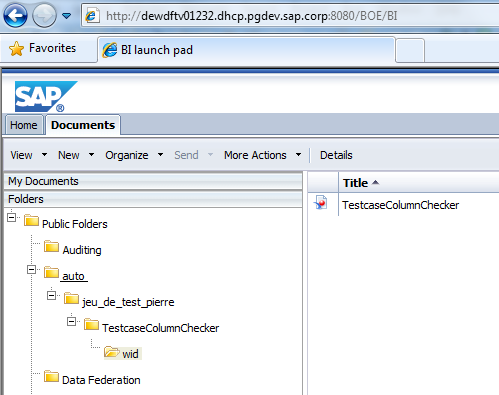
\includegraphics{images/savedReferenceDocPath.png}
  %\caption{Capture d'\'{e}cran de WebI de l'arborescence du document de r\'{e}f\'{e}rence}
	%\label{figure:savedReferenceDocPath}
%\end{figure}
%\begin{figure}[H]
  %\centering
      %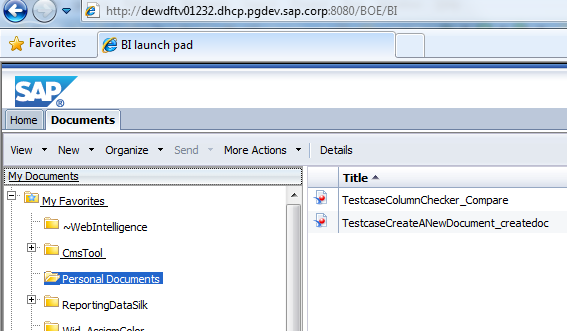
\includegraphics{images/savedGeneratedDocPath.png}
  %\caption{Capture d'\'{e}cran de WebI de l'arborescence du document g\'{e}n\'{e}r\'{e}}
	%\label{figure:savedGeneratedDocPath}
%\end{figure}


\subsection{De l'\'{e}tude \`{a} l'int\'{e}gration}

D'abord, les demandes de tests automatiques ne sont pas toujours r\'{e}alisables au niveau SDK. Il convient donc de v\'{e}rifier, en premier lieu, la faisabilit\'{e} du test. Cette \'{e}tape n\'{e}cessite de particuli\`{e}rement bien conna\^{i}tre le produit pour savoir si telle ou telle action est effectu\'{e} au niveau \gls{SDK}. La m\'{e}thode que j'utilisais \'{e}tait de tester la fonctionnalit\'{e} sur le client DHTML afin de savoir quelles m\'{e}thodes \'{e}taient appel\'{e}es. Ensuite, je me rendais dans le code de Web Intelligence afin de rechercher le code en question. Si les appels en question se faisaient du SDK, je pouvais impl\'{e}menter mon test, sinon, si les appels \`{a} tester se faisaient plus bas dans l'architecture, je ne pouvais pas impl\'{e}menter le test.\\
Cette mani\`{e}re de proc\'{e}der est longue et sa complexit\'{e} ne me garantissait d'arriver \`{a} mes fins. De sorte qu'en r\`{e}gle g\'{e}n\'{e}rale je n'arrivai pas \`{a} trouver la r\'{e}ponse. J'essayais toujours mais je finissais souvent par impl\'{e}menter le test sans savoir si cela serait possible d'en arriver au terme. Cela m'a valu de perdre beaucoup de temps \`{a} impl\'{e}menter des codes qui, au final, n'ont jamais servi.\\

Pour analyser le test automatique \`{a} impl\'{e}menter je devais d'abord aller essayer sur Web Intelligence le \gls{Workflow} qui faisait survenir l'anomalie. Toutes les informations que l'on a sur celle-ci se trouvent sur JCWB\index{\gls{Java} Correction WorkBench} (voir figure \ref{figure:JCWB-CRs} page \pageref{figure:JCWB-CRs}) ou Jira\index{Jira}, je pouvais alors conna\^{i}tre :
\begin{itemize}
	\item L'identifiant du defect (utilis\'{e} par les conventions de nommage)
	\item La description d\'{e}taill\'{e}e du \gls{Workflow} pour faire l'exp\'{e}rience de l'anomalie
	\item La/Les branche(s) sur laquelle/lesquelles elle a \'{e}t\'{e} d\'{e}cel\'{e}e, de mani\`{e}re \`{a} en faire l'exp\'{e}rience deux fois. La premi\`{e}re pour v\'{e}rifier l'existence de l'anomalie et le deuxi\`{e}mement pour valider que celle-ci a \'{e}t\'{e} correctement corrig\'{e}e.
\end{itemize}
\begin{figure}[!ht]
  \centering
      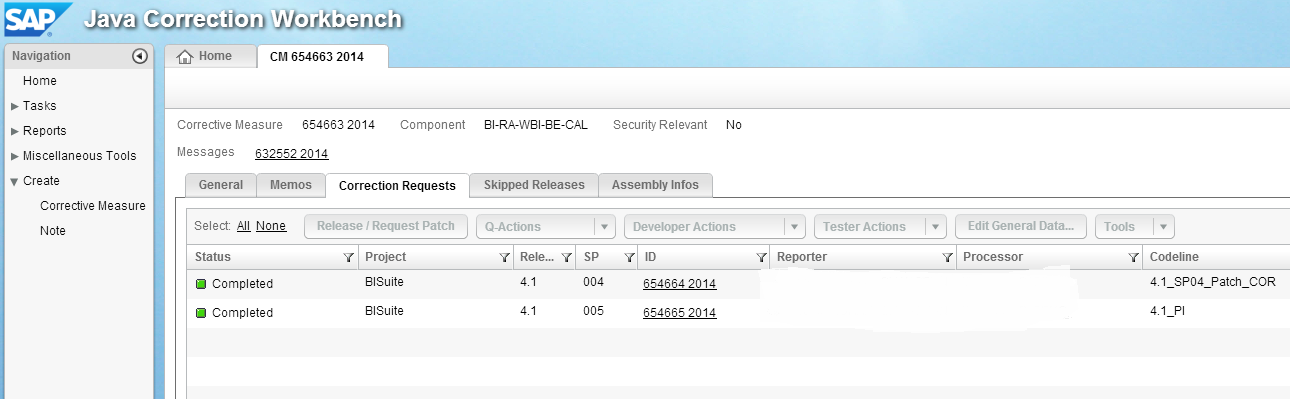
\includegraphics[width=\textwidth]{images/JCWB-CRs.png}
  \caption{\'{E}cran de JCWB propre \`{a} une CM\index{Correction Measure}}
	\label{figure:JCWB-CRs}
\end{figure}

Cette partie pr\'{e}alable \`{a} l'impl\'{e}mentation du test automatique m'a permi de manipuler le produit Web Intelligence et plus particuli\`{e}rement les fonctionnalit\'{e}s que je devais tester. J'ai appris beaucoup de choses sur son utilisation et ses fonctionnalit\'{e}s. \\
Pour cela j'ai du apprendre \`{a} l'utiliser, cr\'{e}er des rapports et effectuer des changements dessus. Web Intelligence est un produit incroyablement riche en fonctionnalit\'{e}s dans lequel il est possible de faire beaucoup de choses. Cette exp\'{e}rience est d'autant plus riche que toutes les connaissances et savoir-faire que j'ai acquis pourront me servir dans le futur. Je suis tr\`{e}s loin de ma\^{i}triser Web Intelligence mais j'ai pu en comprendre l'utilit\'{e} et la logique d'utilisation. Je serai donc capable, \`{a} l'avenir, de faire valoir cette comp\'{e}tence.\\

Lors de mes investigations sur les fonctionnalit\'{e}s et les anomalies, en plus de devoir reproduire le \gls{Workflow} \`{a} la main de puis l'interface graphique, je devais \'{e}tudier les correctifs appliqu\'{e}s pour orienter ma logique d'impl\'{e}mentation du \gls{Testcase}. Cela a \'{e}t\'{e} tr\`{e}s formateur car les diff\'{e}rents codes que j'\'{e}tudiais avaient \'{e}t\'{e} impl\'{e}menter par des d\'{e}veloppeurs confirm\'{e}s. Il est connu que c'est en lisant le code d'autrui que l'on progresse, et j'ai appris \'{e}norm\'{e}ment de choses, tant du point de vu de la logique de la programmation orient\'{e}e objet que de la complexit\'{e} des proc\'{e}dures utilis\'{e}es. De plus, en observant les modifications faitent pour corriger l'anomalie j'ai pu comprendre plus en d\'{e}tail les diff\'{e}rentes raisons qui font qu'une telle anomalie puisse exister (voir l'interface graphique qui me permettait de faire ces observations figure \ref{figure:diffAgainst} page \pageref{figure:diffAgainst}). Ce qui peut-\^{e}tre, entre autre, une condition manquante, un probl\`{e}me d'identifiant ou une m\'{e}moire satur\'{e}e.\\


\begin{figure}[!ht]
  \centering
      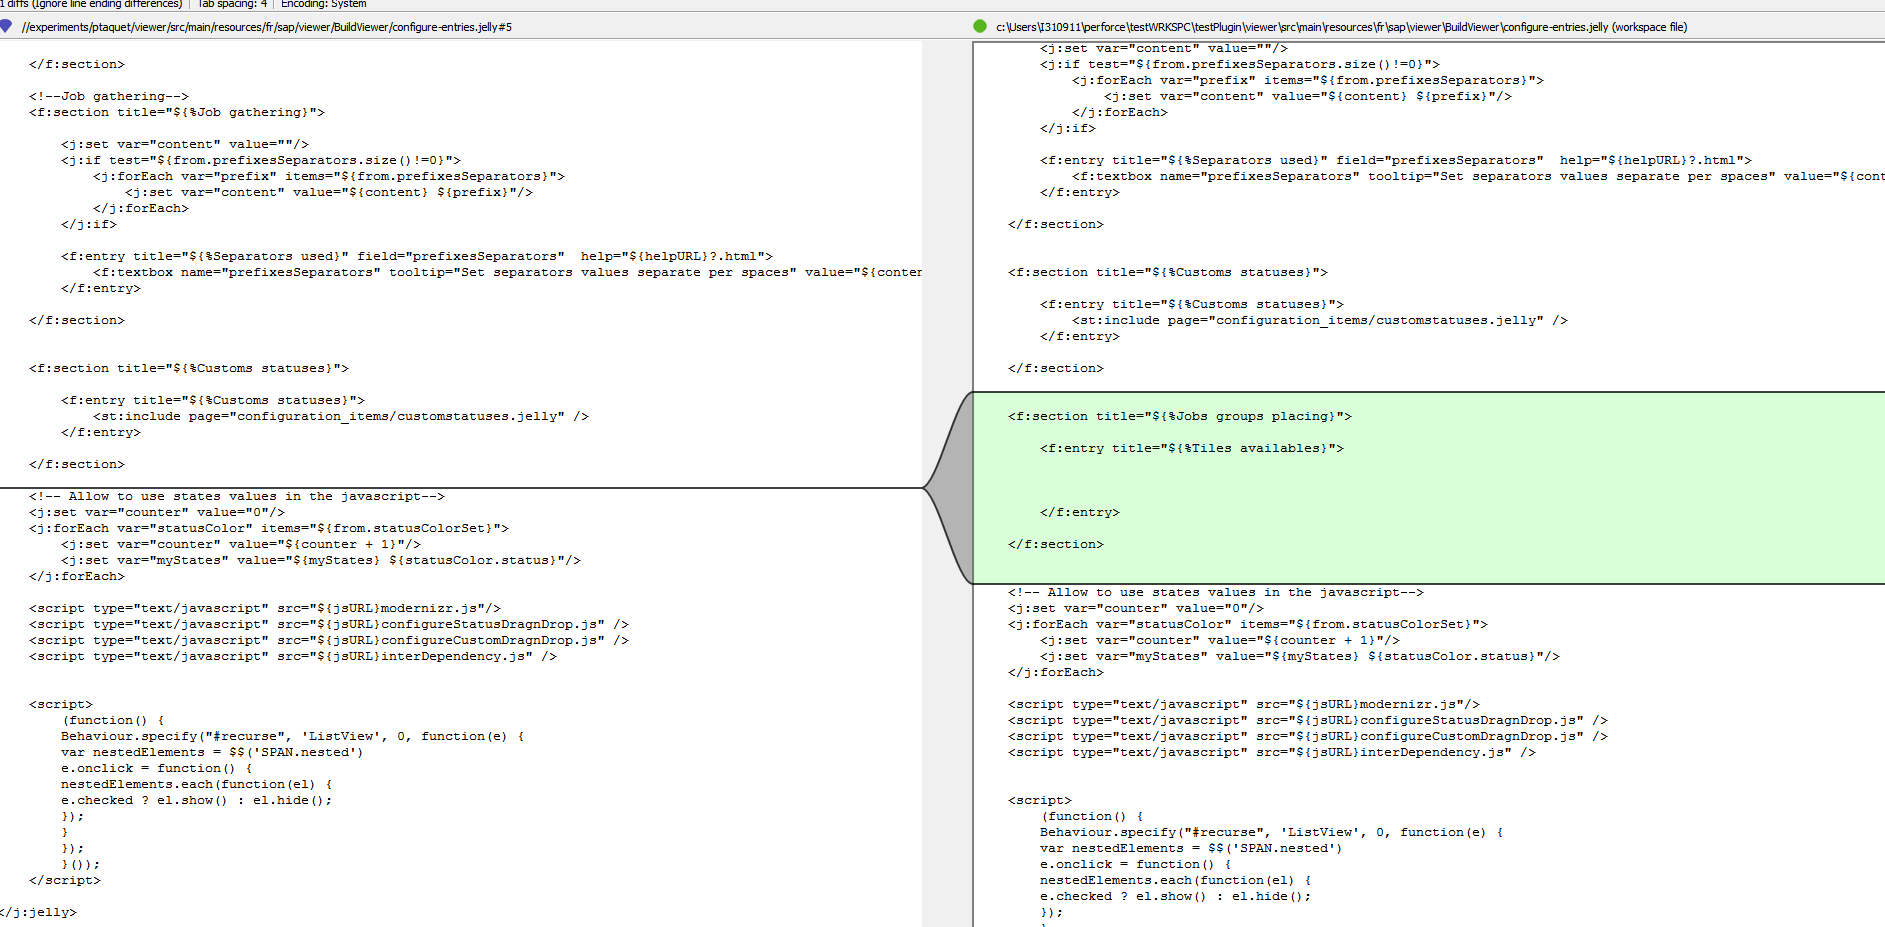
\includegraphics[width=\textwidth]{images/diffAgainst.png}
  \caption{\'{E}cran de comparaison des 2 versions d'un m\^{e}me fichier (avant et apr\`{e}s correctif)}
	\label{figure:diffAgainst}
\end{figure}




\subsubsection{Impl\'{e}mentation de la coquille vide}

Apr\`{e}s avoir fait l'\'{e}tude de l'anomalie, il faut commencer \`{a} impl\'{e}menter le test automatique. La premi\`{e}re difficult\'{e} que j'ai rencontr\'{e} \'{e}tant le choix du point de d\'{e}part, il en existe plusieurs. Mon tuteur m'a guid\'{e} dans le choix de ceux-ci et m'en a expliqu\'{e} les diff\'{e}rents int\'{e}r\^{e}ts. Il \'{e}tait difficile de comprendre comment et pourquoi utiliser l'un ou l'autre car cela d\'{e}pendait directement de ce qui devait \^{e}tre fait dans le test automatique. Si le test portait sur des \'{e}l\'{e}ments graphiques ou des configuration il \'{e}tait plus simple de baser son test sur un document Web Intelligence, car celui-ci me permettait d'appliquer la majeure partie des actions accessibles depuis l'interface graphique. Si je voulais plut\^{o}t v\'{e}rifier un contenu quelconque, il \'{e}tait plus simple de se baser sur une \gls{Queryspec} car toutes les donn\'{e}es y sont directement accessibles. \\
J'ai majoritairement utilis\'{e} les documents Web Intelligence pour d\'{e}marrer mes tests. Mais, une fois, je me suis retrouv\'{e} confront\'{e} \`{a} un probl\`{e}me que je ne pouvais pas r\'{e}soudre car je n'avais pas choisi la queryspec. Je voulais acc\'{e}der \`{a} une information du document qui n'\'{e}tait pas disponible depuis le \gls{SDK}, en utilisant le document Web Intelligence, mais qui l'\'{e}tait depuis la queryspec. J'ai cherch\'{e} pendant de longues heures, en \'{e}tant au plus proche de ce que je cherchais mais malheureusement aux limites de ce que le \gls{SDK} me permettait de faire. Je n'ai jamais r\'{e}ussi \`{a} r\'{e}soudre le probl\`{e}me seul, je suis donc all\'{e} voir mon tuteur pour exposer mon probl\`{e}me, celui-ci m'a expliqu\'{e} le pourquoi de l'obstacle que je rencontrais et m'a conseill\'{e} d'utiliser plut\^{o}t la queryspec. Apr\`{e}s \^{e}tre retourn\'{e} dans mon bureau, j'ai pu r\'{e}soudre mon probl\`{e}me et finir d'impl\'{e}menter mon test automatique avant la fin de la journ\'{e}e.\\
Plus que d'avoir heurt\'{e} les limites du champ d'action du \gls{SDK}, ma principale erreur \`{a} \'{e}t\'{e} de ne pas me dirig\'{e} plus t\^{o}t vers la personne qui aurait pu me conseiller, cela m'aurait \'{e}pargn\'{e} plusieurs heures d'effort inutiles.\\

Le choix du point de d\'{e}part pour impl\'{e}menter un test automatique est donc tr\`{e}s important. Mais quelque soit ce choix, il faut aussi impl\'{e}menter la coquille vide de ce test, qui est, dans tous les cas, quasiment similaire. La coquile vide permet d'avoir un code qui compile mais qui ne fait encore rien. Ce qui garantit que tous les \'{e}l\'{e}ments sont bien reli\'{e}s entre eux. Car, comme sch\'{e}matis\'{e} figure \ref{figure:testsRelations} page \pageref{figure:testsRelations}, chaque test automatique est int\'{e}gr\'{e} \`{a} un \gls{Testplan}, lui-m\^{e}me int\'{e}gr\'{e} \`{a} une \gls{Testsuite}.\\
\begin{figure}[!ht]
  \centering
      
\includegraphics[width=\textwidth]{images/testsRelations.jpg}
  \caption{Diagramme UML des suites de tests}
	\label{figure:testsRelations}
\end{figure}

Les fichiers essentiels au bon fonctionnement du test sont d\'{e}crit ci-dessous. Il n'\'{e}tait pas \'{e}vident, au d\'{e}but, de compl\'{e}ter correctement tous ces documents car chacun ayant une utilit\'{e} tr\`{e}s particuli\`{e}re :
\begin{itemize}
	\item Test plan
	\item Test case
	\item Test suite
	\item script.xml
	\item ressources (\gls{Queryspec}\index{queryspec} ou document Web Intelligence)
	\item parameters.xml
\end{itemize}

La principale difficult\'{e} que j'ai rencontr\'{e} lors de l'impl\'{e}mentation de la coquile a \'{e}t\'{e} la convention de nommage. En effet, la moindre erreur ne permet pas au test de compiler.\\
Pour illustrer la coquille vide du test automatique et pour permettre de les visualiser dans la structure du \gls{Framework}, je les ai repr\'{e}sent\'{e} dans la figure \ref{figure:testEmptyShell} page \pageref{figure:testEmptyShell}. Et, de la m\^{e}me mani\`{e}re, la figure \ref{figure:usedFilesForTests} page \pageref{figure:usedFilesForTests} pr\'{e}sente le test avec les diff\'{e}rents documents avec lesquels celui-ci interagit.\\
Les ressources sont tr\`{e}s importantes dans le contexte du test, et j'ai eu quelques difficult\'{e}s au d\'{e}but pour arriver \`{a} les g\'{e}n\'{e}rer rapidement.\\
Il m'est arriver plusieurs fois de g\'{e}n\'{e}rer des fichiers de r\'{e}f\'{e}rences \`{a} partir de la mauvaise version, ce qui avais pour effet de faire \'{e}chouer mes tests sans que je puisse, rapidement, savoir pourquoi.\\
\begin{figure}[H]
  \centering
      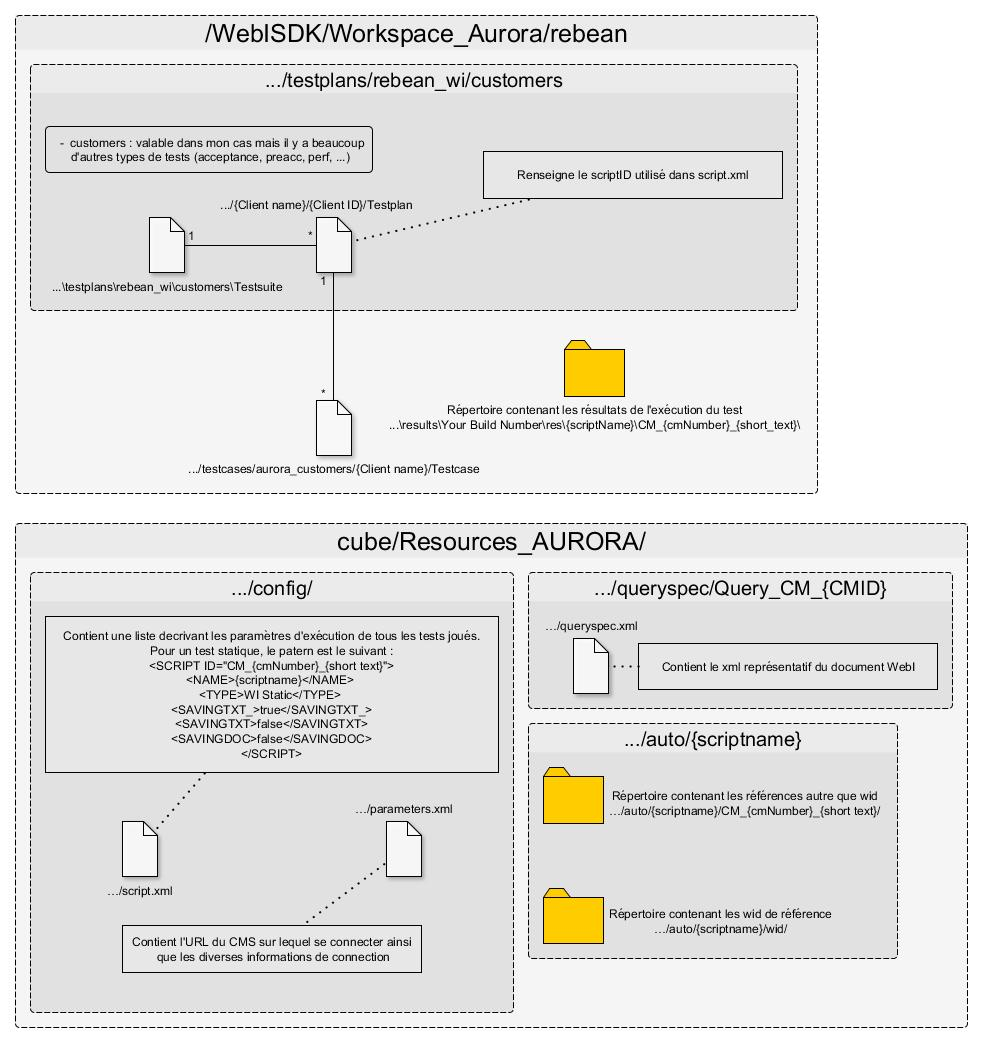
\includegraphics[width=\textwidth]{images/testEmptyShell.jpg}
  \caption{Diagramme repr\'{e}sentant les diff\'{e}rents \'{e}l\'{e}ments qui compose la coquille vide d'un test dynamique}
	\label{figure:testEmptyShell}
\end{figure}
\begin{figure}[H]
  \centering
      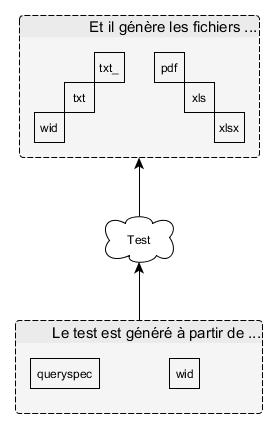
\includegraphics[width=0.4\textwidth]{images/usedFilesForTests.jpg}
  \caption{Les fichiers utilis\'{e}s ou g\'{e}n\'{e}r\'{e}s par le test}
	\label{figure:usedFilesForTests}
\end{figure}

\subsubsection{Les ressources}

Comme j'en ai d\'{e}j\`{a} parl\'{e} plus haut, il existe plusieurs types de ressources. Les deux principales \'{e}tant le document Web Intelligence et la \gls{Queryspec}.
Il y a deux mani\`{e}res d'obtenir un document Web Intelligence, les deux sont similaires
\textbf{Obtenir un fichier wid\index{wid}}
\begin{description}
	\item	[Via le CMS\index{CMS}] 
	\begin{sloppypar}
	Il suffit de parcourir l'arborescence du CMS\index{CMS} pour arriver \`{a} l'emplacement du .wid\index{wid}. Dans les propi\'{e}t\'{e}s du fichier, il y a son nom complet (diff\'{e}rent du nom dans WebI) avec son arborescence \`{a} partir du dossier Input (figure \ref{figure:widFileLocation} page \pageref{figure:widFileLocation} ). Ensuite, dans le syst\`{e}me de fichiers du serveur (par exemple : \textquote{\textbackslash{}\textbackslash{}dewdftv01634.dhcp.pgdev.sap.corp\textbackslash{}c\$}) aller dans 
	\textquote{\textbackslash{}Program Files (x86)\textbackslash{}SAP BusinessObjects\textbackslash{}SAP BusinessObjects Enterprise XI 4.0\textbackslash{}FileStore\textbackslash{}Input} et copier/coller le chemin d'acc\`{e}s au fichier. Le document Web Intelligence se trouve dans le r\'{e}pertoire en question.
	\end{sloppypar}
\begin{figure}[!ht]
  \centering
      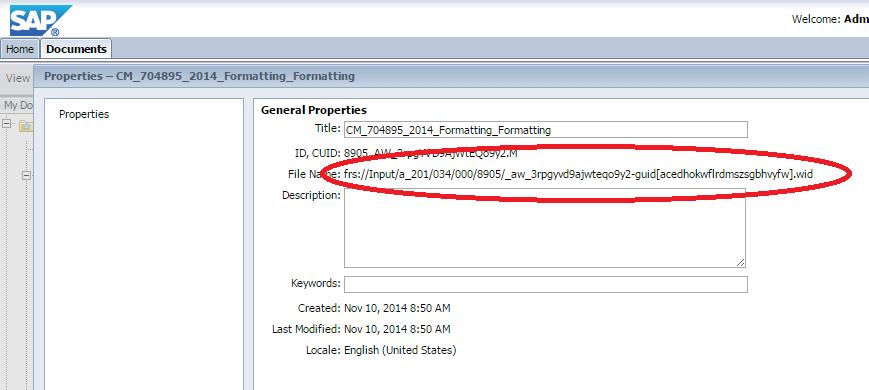
\includegraphics[width=\textwidth]{images/widFileLocation.png}
  \caption{Capture de l'\'{e}cran de propri\'{e}t\'{e} d'un document WebI}
	\label{figure:widFileLocation}
\end{figure}
	\item[Via le Rich Client]
	Avec ce proc\'{e}d\'{e} il faut faire attention \`{a} la version du rich client qui doit \^{e}tre la m\^{e}me que celle du CMS\index{CMS}, une erreur se traduit par un fichier de r\'{e}f\'{e}rence erron\'{e}, donc un test qui \'{e}choue. J'ai fais cette erreur plusieurs fois, au d\'{e}but, car j'avais toujours plusieurs versions de Web Intelligence qui \'{e}taient ouvertes. L'utilisation du \gls{Client lourd} est la plus instinctive car il suffit d'ouvrir le document et de l'enregistrer en local.
\end{description}






%\clearpage
\section{Bilan de la 1\up{\`{e}re} p\'{e}riode}
Tout au long des mois de juillet, ao\^{u}t et septembre j'ai impl\'{e}ment\'{e} de nombreux tests\footnote{cf. annexe \ref{pdf:ImplementedTestsList} page \pageref{pdf:ImplementedTestsList} pour la liste compl\`{e}te des tests impl\'{e}ment\'{e}s} pour des bugs divers, que ce soit une faute de frappe ou un dysfonctionnement. J'ai beaucoup appris de mes erreurs, surtout lorsque plusieurs jours de travail s'av\'{e}raient inutiles parce qu'une meilleure solution, \'{e}vidente pour qui sait, existait.\\
J'ai aussi pu parfaire mes connaissances en Java ainsi que ma m\'{e}thodologie lorsque je dois me former \`{a} une nouvelle technologie.\\
Au d\'{e}but de cette mission, je n'avais jamais impl\'{e}ment\'{e} de tests \`{a} l'exception de tests unitaires. Aujourd'hui, je suis ravi de comprendre la probl\'{e}matique du test et quels types de tests existent. Aujourd'hui je sais pourquoi et comment les impl\'{e}menter et suis capable de faire des tests qui soient facilement maintenables.




\subsection{Connaissance du framework}
La principale perte de temps \'{e}tait d\^{u}e \`{a} une m\'{e}connaissance du Framework de test. Celui-ci poss\'{e}dant un grand nombre de m\'{e}thodes aux int\'{e}r\^{e}ts divers et vari\'{e}s, d'embl\'{e}e, il est tr\`{e}s difficile de pouvoir d\'{e}terminer laquelle utiliser. D'autant plus qu'au moment o\`{u} le besoin de telle ou telle m\'{e}thode se faisait sentir, je n'avais pas connaissance de son existence. En cons\'{e}quence, je me suis vu trop souvent impl\'{e}menter des m\'{e}thodes d\'{e}j\`{a} existantes, me faisant perdre un temps pr\'{e}cieux.\\
L'exp\'{e}rience accumul\'{e}e durant cette p\'{e}riode m'a permis de ne plus perdre de temps \`{a} r\'{e}-inventer la roue et de me concentrer sur le code ad hoc n\'{e}cessaire \`{a} un test pr\'{e}cis et fiable.

\subsection{M\'{e}thodologie}
L'autre grande perte de temps venait surtout de ma m\'{e}connaissance du produit test\'{e}. Certaines fonctionnalit\'{e}s \'{e}tant tr\`{e}s complexes il m'arrivait de ne pas identifier exactement le probl\`{e}me pour finalement perdre du temps \`{a} impl\'{e}menter du code inefficient.\\
Le meilleur exemple que je puisse citer s'est produit quand j'ai commenc\'{e} \`{a} tester des bugs int\'{e}gr\'{e}s \`{a} des workflows complexes. Un certain nombre de manipulations et/ou de configurations \'{e}tait alors n\'{e}cessaire pour que le bug survienne. Et c'est dans ces conditions que j'ai impl\'{e}ment\'{e} la quasi totalit\'{e} du workflow au niveau SDK pour finalement arriver sur la zone \`{a} tester. Le test fonctionnait bien, il \'{e}chouait sur les versions bugg\'{e}es et passait sur les versions fix\'{e}es. Le probl\`{e}me ne vient pas du test que j'ai impl\'{e}ment\'{e}, car celui-ci faisait ce qu'il fallait, mais de la mani\`{e}re. J'ai impl\'{e}ment\'{e} ce code en approximativement 3 jours. Alors que si j'avais utilis\'{e} le CMS pour g\'{e}n\'{e}rer un document \`{a} une \'{e}tape seulement du bug, et que si j'avais impl\'{e}ment\'{e} uniquement l'appel \`{a} tester, j'aurais pu impl\'{e}menter ce test en quelques heures seulement!

\subsection{Travail en \'{e}quipe}
Le framework de test est entretenu quotidiennement par des dizaines de testeurs impl\'{e}mentant des tests et modifiant le framework lui-m\^{e}me. Le r\'{e}sultat de l'ex\'{e}cution des suites de tests est visible par testeurs, d\'{e}veloppeurs et par d'autres. J'\'{e}tais donc int\'{e}gr\'{e} \`{a} une grande \'{e}quipe, leurs travaux ayant des r\'{e}percussion sur les miens, et les miens sur les leurs. Il faut donc faire attention au code que l'on \textquote{push} sur Perforce! L'anecdote me venant \`{a} l'esprit s'est pass\'{e}e un vendredi soir, alors que je venais de terminer un test et que celui-ci se comportait bien. J'ai livr\'{e} mon test sur Perforce. L'ennui \'{e}tait que j'utilisais un package dans lequel je mettais des m\'{e}thodes de test pour ne pas polluer mon test \textquote{final}. Je n'ai malheureusement pas pens\'{e} \`{a} revoir l'import de mes sources. Mon code, compilant correctement en local, ne compilait plus sur le serveur et a donc fait crash\'{e} toute la suite de test. Le mail automatique envoy\'{e} a inform\'{e} tout le monde de mon erreur de manipulation (illustr\'{e}e annexe \ref{annexe:crashedBuildBecauseOfMe} page \pageref{annexe:crashedBuildBecauseOfMe})!\\

J'ai eu aussi la chance de travailler dans une \'{e}quipe maitrisant tr\`{e}s bien le framework et le produit. J'ai appris \'{e}norm\'{e}ment pendant les entretiens que j'ai eu avec ces diff\'{e}rentes personnes.



%\chapter{Migration Jira/Java Correction WorkBench}\label{chapitre:migration}

\section{Qu'est-ce que Jira et Java Correction WorkBench (JCWB)}
Jira\index{Jira} est un logiciel de tra\c{c}abilit\'{e} des probl\`{e}mes d\'{e}veloppé par Atlassian dont l'usage est gratuit pour les organisations \`{a} but non lucratif, de charit\'{e} ou les projets open-source. SAP désire migrer de système de traçabilité pour utiliser maintenant Java Correction WorkBench\index{Java Correction WorkBench} (JCWB ou CWB).\\

JCWB est un logiciel interne à SAP dont l'utilisation à été imposée par la hiérarchie, son domaine d'utilisation est la gestion des corrections. Historiquement, SAP utilise Jira pour gérer le projet, les problèmes (defects) et les corrections.\\
La stratégie de gestion des bugs changeant, SAP a pris la décision d'utiliser un seul et même outil de gestion des problèmes en interne comme en externe (à l'usage des clients) : BCP. Cet outil permet de renseigner un problème, quel qu'il soit, et s'il s'avère que ce problème est un bug logiciel il est transféré vers JCWB, qui suivra ce bug toute la durée de la correction.

%ASTEC est un logiciel interne à SAP dont la première version est sortie en 2007. ASTEC



\section{Pr\'{e}sentation du contexte}


\`{A} SAP, tous les codes des différents projets sont hébergés sur le gestionnaire de version Perforce\index{Perforce} (SCM : Source Code Management)
et ceux-ci sont compilés plusieurs fois par jour grâce à Jenkins\index{Jenkins} ou ASTEC (CIS : Continuous Integration Software).\\
Chaque projet est constitué de deux choses distinctes, d'une part, son code source et, d'autre part, les tests joués pour garantir\footnote{La valeur de la garantie dépend directement du test coverage} le bon fonctionnement du produit. Lorsqu'il y a un problème sur la build, que ce soit une erreur de compilation ou un test qui échoue, le statut de la build change pour être représentatif du problème. Dès lors que quelqu'un s'en aperçoit, il inscrit un defect\index{Defect} dans Jira\footnote{L'utilité de Jira est bien plus large que la simple déclaration d'un test échoué, il sert à décrire n'importe quel problème quelle que soit la version, la branche ou le produit} ou dans JCWB.\\


\subsection{Plugin de reporting}
Pour leur permettre d'avoir un rapport visuel sur l'état des builds, ils utilisent le plugin Radiator. Ce plugin permet l'affichage, sur un seul écran divisé, des groupes de jobs\footnote{Typiquement, un job correspond à un projet logiciel}. Un groupe de jobs est un carré coloré dont la couleur représente l'état des jobs qui le compose, voir la capture d'écran figure \ref{figure:radiatorActual} page \pageref{figure:radiatorActual}.\\
Les statuts pris en compte sont les statuts Jenkins\footnote{Error, Failure, Unstable, Aborted, Not built, Success} ainsi qu'un statut supplémentaire issue du plugin Claim. Ce plugin permet à un développeur de \textquote{claimer} une erreur, c'est-à-dire, ajouter au projet une information supplémentaire : le nom de l'utilisateur qui a \textquote{claimer} et le message que celui-ci a laisser aux visiteurs suivants.




\begin{figure}[!h]
  \centering
      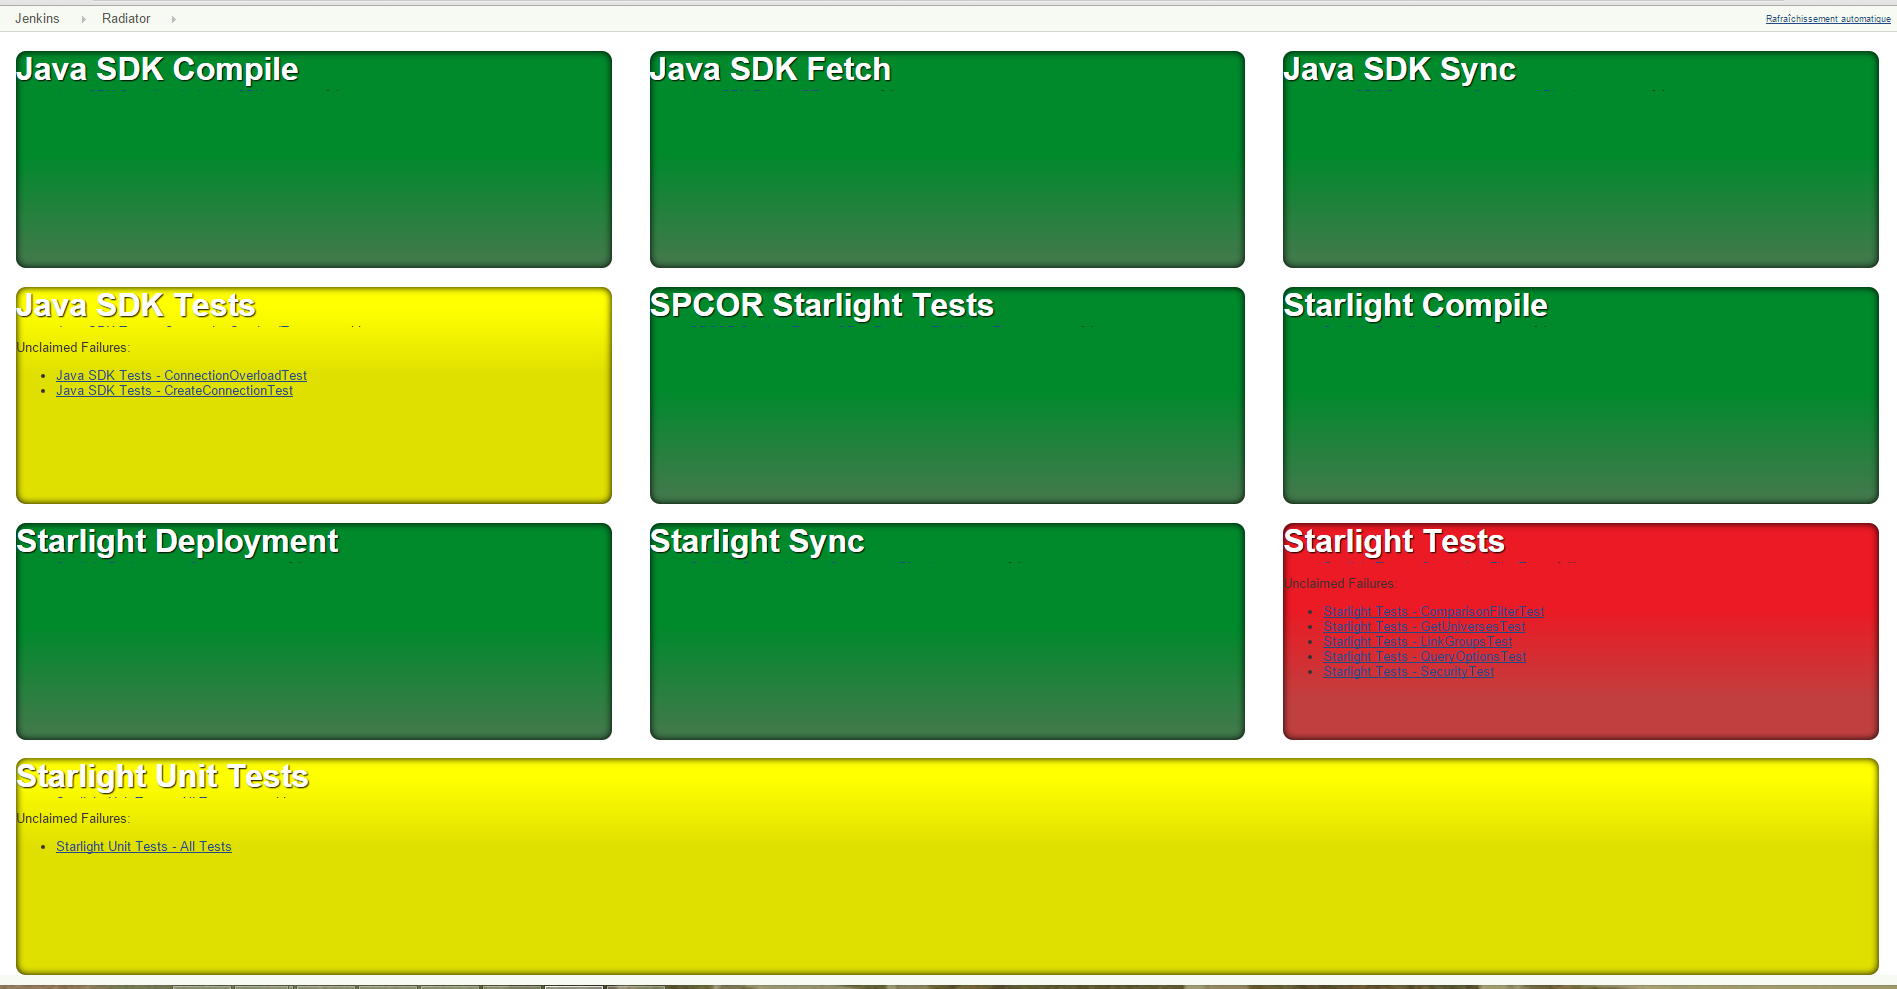
\includegraphics[width=\textwidth]{images/radiatorActual.png}
  \caption{Plugin Radiator utilisé actuellement}
	\label{figure:radiatorActual}
\end{figure}

En résumé Radiator :
\begin{itemize}
	\item permet de rassembler les jobs en un seul groupe de jobs
	\item où chacun des jobs a un statut\footnote{statut propre à Jenkins}
	\item que le groupe de projet arbore la couleur représentative du statut jugé le plus important
	\item permet de prendre en compte les informations supplémentaires du plugin claim
\end{itemize}
Par exemple, si nous avons deux groupes composés chacun de trois jobs, tous différents. Supposons que, sur les 6 jobs, l'un soit en échec les autres étant en succès. Nous aurons donc une vue colorée en verte (parce que tous les projets sont en succès) et la deuxième vue apparaissant en rouge (l'un des jobs ayant échoués) ou bien en orange si l'échec est investigué (échec claim par un développeur).\\
La figure \ref{figure:RadiatorInformationSources} page \pageref{figure:RadiatorInformationSources} illustre bien les sources d'informations du plugin. Il puise ses résultats depuis Jenkins et le plugin claim, les résultats de Jenkins puisant ses résultats en partie des résultats de tests JUnit.\\
L'inconvénient de ce procédé est que lorsque qu'un test a échoué, tout le groupe de test passe en rouge. Dans cette situation, il devient impossible de détecter les nouveaux tests qui échouent.




\begin{figure}[!h]
  \centering
      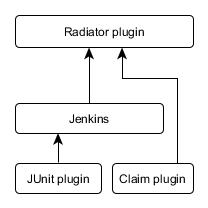
\includegraphics[scale=0.5]{images/RadiatorInformationSources.jpg}
  \caption{Contexte du'utilisation du plugin Radiator utilisé actuellement}
	\label{figure:RadiatorInformationSources}
\end{figure}




La solution simple et provisoire, mais permettant de contourner le problème et de ne plus polluer l'affichage avec du rouge, consiste à faire passer les jobs en échec avec defect\index{Defect} (ie. reconnus et enregistrés comme échecs dans Jira\index{Jira} ou CWB\index{Java Correction WorkBench}) en vert.\\
De cette manière, puisque seuls les nouveaux échecs apparaissent en rouge, toute régression est visible immédiatement.\\
Cette transformation est mise en \oe{}uvre grâce à une annotation, celle-ci est présentée figure \ref{figure:annotationJava} page \pageref{figure:annotationJava}.\\


\begin{figure}[h]
  \centering
      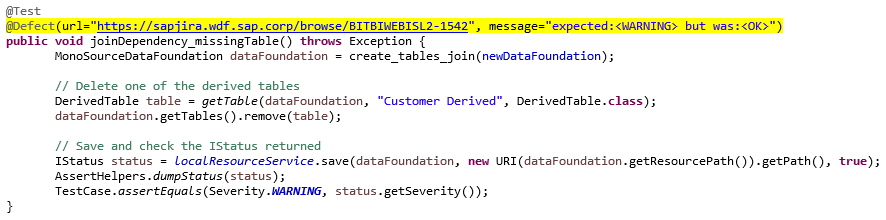
\includegraphics[width=\textwidth]{images/annotationJava.png}
  \caption{Annotation utilisée pour vérifier le statut du defect Jira}
	\label{figure:annotationJava}
\end{figure}

De cette manière le test est relié au defect et si :
\begin{enumerate}
	\item le test est échoué mais le statut est \textquote{Active} ou \textquote{Open}
	\item le message d'erreur match\footnote{} avec celui attendu
\end{enumerate}
\textbf{Alors}, le test sera considéré en succès par Jenkins. Ensuite, quand un développeur livrera le fix, le defect passera à \textquote{Validate}, ce qui court-circuitera l'annotation\footnote{même comportement pour le statut \textquote{Closed} ou n'importe quel autre qui n'est pas \textquote{Active} ni \textquote{Open}}. Et en fonction de l'efficience du fix, le test redevient vert ou reste à rouge.\\
\textbf{De cette manière}, seuls les tests non investigués sont rouges, ce qui permet de réagir beaucoup plus rapidement et de réduire le temps d'investigation.\\

Pour résumer, la relation qu'entretien BCP et JCWB est illustrée figure \ref{figure:bugManagementProcess}.

\begin{figure}[h]
  \centering
      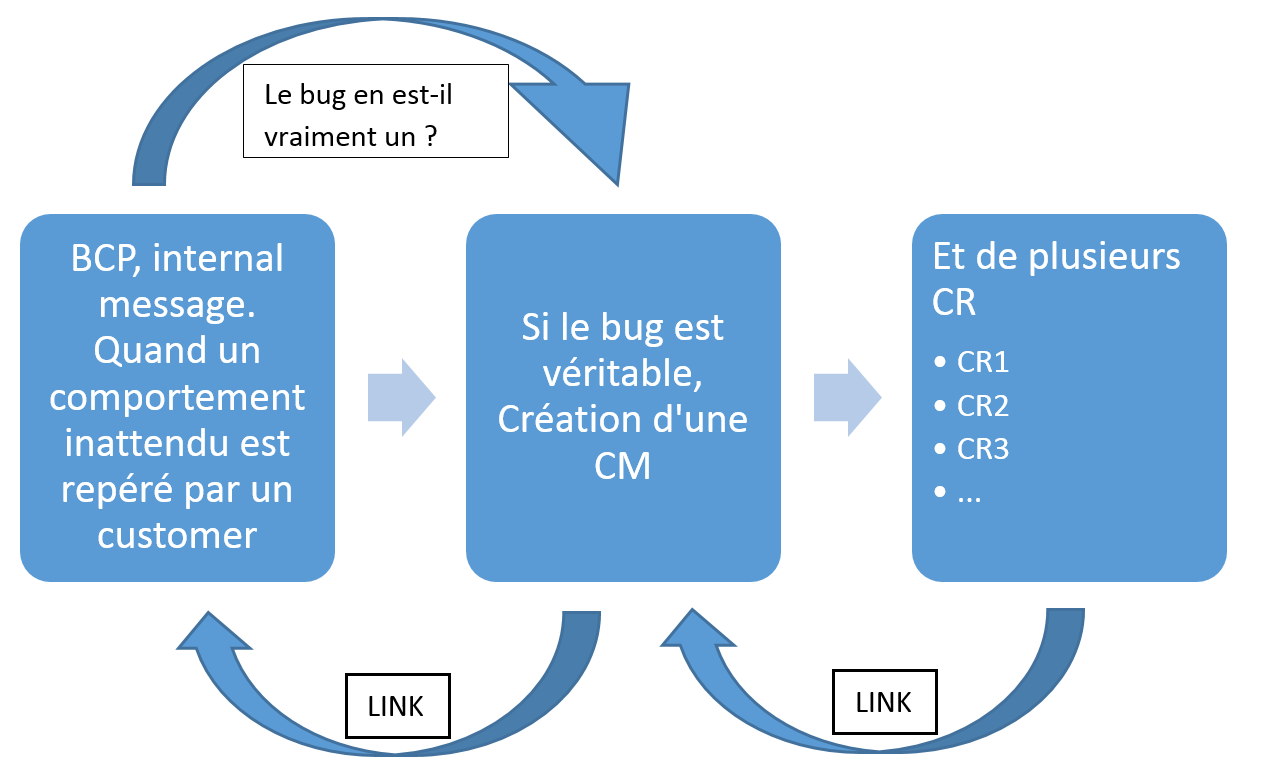
\includegraphics[width=\textwidth]{images/bugManagementProcess.png}
  \caption{Process de gestion de bug utilisé}
	\label{figure:bugManagementProcess}
\end{figure}




\textbf{Problématique}\hfill \\ \indent

Actuellement, seuls les defects rentrés sur Jira sont pris en compte, la mécanique en place ne permet pas de récupérer ces mêmes informations de JCWB\index{Java Correction WorkBench}. \\
Puisque de plus en plus de defects seront enregistrés sur JCWB, et dans un soucis d'homogénéisation du process actuel, il faut mettre à jour le process actuel et permettre aux statuts d'être ajustés quelque soit l'origine du defect (Jira ou CWB).\\
La problèmatique supplémentaire relève de l'architecture différente différente de Jira et de BCP\footnote{Contient le message initial à l'origine du defect} + JCWB\footnote{Contient la \textquote{Correction Measure} (CM) et les \textquote{Correction Requests}} (CR), ce qui nous oblige à aller receuillir des informations à deux endroits différents. Le premier objectif étant de récupérer l'identifiant de la \textquote{Correction Request} à laquel le defect est associé et l'identifiant de la \textquote{Correction Measure} à laquel la CR est associée.\\






\section{Travail effectué}


La première partie du travail s'est cantonée d'abord à des échanges de mails parallèlement à des recherches.\\
Les différentes choses essentielles à mon projets sont les suivantes :

\begin{itemize}
	\item il existe un web service permettant de récupérer les informations d'une CR : CWB HTTP API
	\begin{itemize}
		\item l'utilisation de ce web service se fait via une authentification normalisée par SAP : PROD-PASS-ACCESS
	\end{itemize}
	\item le fichier à implémenter pour compléter le comportement actuel est JiraIssueWatcher.java	
\end{itemize}




\subsection{Fonctionnement et utilisation de prod-pass-access}



\subsection{Son utilisation depuis Java}



\section{Résultats obtenus}
Maintenant cette mission achévée, nous pouvons récupérer les informations relatives au statut d'un defect, quelque soit son emplacement (Jira ou CWB), depuis test-defects.xml.



-> connaissances Java
J'ai approfondi mes connaissances sur les annotations et la manière de les implémenter.
J'ai implémenté ma première classe abstraite 


%\chapter{Plugin Jenkins}

\section{Contexte initial}

Jenkins est un logiciel d'intégration continue, il est utilisé à SAP dans le contexte des tests . Son rôle est d'intégrer les différents projets, tels que configurés par l'utilisateur, et de mettre à disposition les résultats obtenus. Il permet d'avoir un retour régulier sur l'état des builds et du résultat de leurs tests.\\

Un plugin permettant une vision globale sur l'état des builds est déjà en place, Radiator. La figure \ref{figure:reportingPluginEnvironmentAfter} page \pageref{figure:reportingPluginEnvironmentAfter} présente son environnement d'utilisation. Nous pouvons y voir les développeurs et les ST qui alimentent le code hébergé sur Perforce que Jenkins l'utilise dans ses diverses intégrations. Au centre, le plugin permet un retour visuel rapide des livraisons Perforce.\\
Ce plugin est aussi conçu pour fonctionner avec un autre plugin, le plugin Claim. Il permet à quelqu'un visitant la page d'un job en échec de le \textquote{claimer}, inscrivant son identifiant ainsi qu'un message à destination de quiconque visiterait cette même page. Ceci permet de signaler que l'investigation est en cours.\\

\begin{figure}[!h]
  \centering
      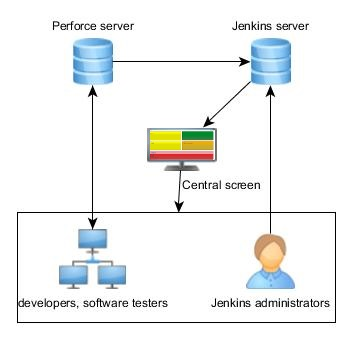
\includegraphics{images/reportingPluginEnvironmentAfter.jpg}
  \caption{L'environnement d'utilisation du plugin}
	\label{figure:reportingPluginEnvironmentAfter}
\end{figure}

Pour résumer ses caractéristiques principales, c'est un plugin qui permet :
\begin{itemize}
	\item d'afficher un écran  où chaque couleur correspond à un statut de build
	\item de rassembler les jobs par leurs préfixes communs
	\item de prendre en compte les claims
\end{itemize}

L'inconvénient est que le nombre de statut existant ne permet pas la précision nécessaire pour définir l'état d'un jobs. Le plugin Radiator n'offre pas la malléabilité nécessaire. Voici la liste des différents états gérés par ce plugin : 
\begin{description}
	\item[SUCCESS] Le projet compile correctement et tous les tests sont passés
	\item[ABORTED] La compilation a été arrêtée en cours d'exécution
	\item[FAILURE] Le code ne compile pas
	\item[ERROR]
	\item[NOT BUILT] Le projet n'a pas été compilé
	\item[UNSTABLE] Des tests JUnit ne sont pas passés mais le code compile
	\item[CLAIM] Le job en échec a été claim par quelqu'un
\end{description}



Tel qu'il se présente le plugin ne permet pas de donner des informations autres que celles issues de Jenkins ou du plugin Claim. Il ne permet donc pas de donner de renseignements sur le defect associé à ce job. Tenir compte du defect permettrait de faire ressortir les régressions et autres erreurs, séparant ainsi les échecs pris en charge de ceux qui ne le sont pas.\\
Suite à la mission précédente, nous avons maintenant accès aux informations relatives aux defects (celles-ci sont enregistrées dans les archives des builds sur le serveur Jenkins), dans un fichier XML que nous avons nommé test-defects (exemple page \pageref{testdefectxml}). Par contre, l'affichage n'est pas représentatif de la réalité, une partie de l'information est perdue puisqu'un test échoué avec defect apparaît en vert (succès).\\




\textbf{La solution propos\'{e}e}\hfill \\ \indent
Dans un 1\up{er}, et en tant qu'exercice, il faudra réaliser un plugin offrant les mêmes possibilités d'affichage des status des builds que Radiator. C'est-à-dire rassembler les jobs par préfixe et afficher le résultat général de tous ces groupes ainsi créés sur un unique écran. Ajouté aux caractéristiques, ce plugin doit pouvoir prendre en compte les informations du plugin Claim.\\ \indent
Dans un second temps, il faudra pouvoir ajouter un ou plusieurs statut(s) supplémentaire(s) et ré-ajuster leur ordre de priorité. L'ajout de ce nouveau statut doit être générique de sorte qu'un statut quelconque puisse être ajouté.\\
Le plugin est donc capable de receuillir des informations dans des fichiers sans savoir au préalable, comment seront structurées ces données. Rappelons que, lors de l'exécution des tests, un fichier test-defect est généré contenant la liste\footnote{Au format xml} des jobs avec defect (exemple page \pageref{testdefectxml}).


\lstinputlisting[language=java,label=testdefectxml]{scripts/test-defects.xml}


\subsection{Organisation du travail}
meeting hebdomadaire avec manager pour faire le point sur l'évolution du projet et fixer les nouveau objectifs.\\
Code review hebdomadaire avec Fabien


\section{\'{E}tude préalable}
Les 1\up{er} impératifs ont été de maitriser le langage et les outils qui me permettraient de mener ce projet à terme. Je n'avais jamais entendu parler de Jenkins ou d'un quelconque logiciel d'intégration continue, et a forciori sur la manière de l'étendre. 


Il existe un archétype maven (cf annexe \ref{annexe:maven} page \pageref{annexe:maven}) permettant de générer le squelette d'un plugin Jenkins.\\

J'ai donc commencé par installer Jenkins et ses plugins, tels qu'ils sont utilisés à SAP, de manière à me familiariser avec ceux-ci. Pour examiner le comportement de Jenkins, j'ai créé de faux projets me permettant de simuler les différents états possibles. Ceux-ci m'ont permis d'observer les différences entre les statuts Jenkins et JUnit, certains statuts portent les mêmes noms mais ne signifient pas les mêmes choses, provoquant quelques incompréhensions. La signification de ces statuts étant l'objet de ce plugin, il m'incombait de les comprendre. Voici le détail des configurations que j'ai testé pour déterminer l'équivalence statut JUnit/statut Jenkins :

\vspace{0.5cm}

\begin{tabular}{|l|rr|c|c|}
	\hline
  \textbf{Description du projet} 							& \textbf{Status JUnit} 	& \textbf{Statut Jenkins}\\
  \hline
  projet vide et sans test 						& NA 						& Success\\
	
	projet vide et avec test réussi			& Passed				& Success\\
  
  projet vide avec test qui échoue 		& Failure				& Unstable\\
	
  projet avec erreur de compilation 	& NA						& Error\\
  \hline
\end{tabular}

\vspace{0.5cm}

Passée cette étape d'installations et de configurations, je me suis penché sur la marche à suivre pour implémenter un plugin Jenkins.\\
La principale difficulté que j'ai eu à développer ce plugin a été de trouver l'information, il est reconnu sur internet que la documentation de Jenkins, lorsque l'on veut l'étendre, n'est pas claire. Mais la documentation officielle\footnote{\url{https://wiki.jenkins-ci.org/display/JENKINS/Extend+Jenkins}} offre un bel état des lieux de ce qu'il est possible de faire, décrit les différentes technologies constituant Jenkins et offre un tutoriel trivial mais suffisant pour comprendre les bases.\\



\section{Le 1\up{er} plugin}

Je me suis d'abord rendu sur la page du tutoriel officiel de Jenkins\footnote{\url{https://wiki.jenkins-ci.org/display/JENKINS/Plugin+tutorial}} afin d'obtenir un plugin fonctionnel avec lequel je pouvais faire mes expériences. Ensuite j'ai suivi un autre tutoriel\footnote{\url{https://cleantestcode.wordpress.com/2013/11/03/how-to-write-a-jenkins-plugin-part-1/}} non-officiel mais considérablement plus riche.\\

\subsection{Le squelette du plugin}
\subsubsection{Configuration}
D'après toutes les documentations disponibles, le meilleur moyen de commencer le développement du plugin est d'utiliser maven\footnote{Maven 3 et JDK 6 ou plus récent} pour générer le squelette. Maven a besoin de configurations supplémentaires dans son settings.xml\footnote{Situé dans le répertoire \texttildelow/.m2} pour pouvoir récupérer les sources relatives à Jenkins.\\
Dans \textquote{pluginGroups} il faut ajouter la ligne suivante :
\begin{lstlisting}
<pluginGroup>org.jenkins-ci.tools</pluginGroup>
\end{lstlisting}
Et dans \textquote{profiles} il faut ajouter le profil suivant :
\begin{lstlisting}[language=xml]
<profile>
<id>jenkins</id>
<activation>
<activeByDefault>false</activeByDefault>
</activation>
<repositories>
<repository>
<id>repo.jenkins-ci.org</id>
<url>http://repo.jenkins-ci.org/public/</url>
</repository>
</repositories>
<pluginRepositories>
<pluginRepository>
<id>repo.jenkins-ci.org</id>
<url>http://repo.jenkins-ci.org/public/</url>
</pluginRepository>
</pluginRepositories>
</profile>
\end{lstlisting}

L'attribut de la balise \textquote{activeByDefault} est à false, parce qu'on travaille avec d'autres profils sur d'autres projets. Mais il faut retenir que ce paramètre peut empêcher la génération du squelette du plugin via la commande :
\begin{lstlisting}[language=xml]
mvn hpi:create
\end{lstlisting}

Pour exécuter la commande ci-dessus, il faut se placer dans le dossier qui recevra le projet. 


\subsubsection{Génération du squelette}
\`{A} l'exécution de cette commande, il est demandé de renseigner le groupId et l'artifactId, le groupId peut être  org.jenkins-ci.plugins et l'artifactId est le nom du plugin. Cette commande crée l'arborescence du projet ainsi que les fichiers de base. 


\`{A} la génération du squelette du plugin nous obtenons un plugin qui compile, dont l'architecture est présentée figure \ref{figure:hpiCreate} page \pageref{figure:hpiCreate}. Certaines choses importantes sont à noter, le pom.xml\footnote{Project Object Model} est généré à la base du projet dans lequel nous trouvons des informations telles que le parent de ce projet, les dépendances, l'auteur, la licence et la description.

\begin{figure}[h]
  \centering
      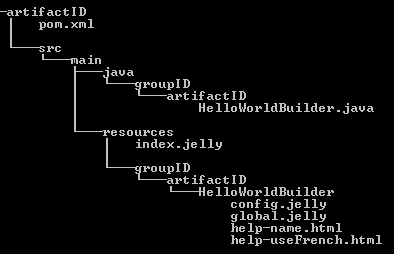
\includegraphics{images/hpiCreate.png}
  \caption{Architecture d'un plugin Jenkins généré par maven}
	\label{figure:hpiCreate}
\end{figure}


%\vspace{\stretch{1}}
Plusieurs autres fichiers sont générés :

\begin{tabular}{|l|p{0.7\linewidth}|}
  \hline
  \textbf{Nom du fichier} & \textbf{Description} \\
  \hline
  index.jelly & Description utilisée à la création d'une nouvelle instance du plugin \\
  config.jelly & Correspond à la page d'une instance du plugin \\
  global.jelly & Correspond à la page de configuration générale du plugin \\
  HelloWorldBuilder.java & Implémentation d'exemple du plugin \\
  help-name.html & Fichier d'aide à la configuration lorsque clic sur le symbole d'aide \\
  help-useFrench.html & Fichier d'aide à la configuration lorsque clic sur le symbole d'aide \\
  \hline
\end{tabular}


\subsubsection{Déploiement du squelette du plugin}
Plusieurs solutions s'offrent à nous pour déployer le plugin dans son environnement d'utilisation

\textbf{Installation \textquote{\`{a} la main}}\hfill \\ \indent 
En ligne de commande et depuis la racine du projet\footnote{\`{a} l'emplacement du POM.xml}, il faut exécuter la commande suivante :
\begin{lstlisting}
mvn clean install -Pjenkins
\end{lstlisting}
Celle-ci va télécharger les sources nécessaires, les compiler, exécuter les tests et, si tout se passe bien, générer le fichier .hpi dans le dossier target.\\
Ceci fait, il faut se rendre dans Jenkins (par exemple http://localhost:8080/ ou autre. En fonction de la configuration), s'identifier et aller dans les paramètres avancés de gestion de plugins. Ici, il faut renseigner le chemin d'accès vers le .hpi et terminer.\\


\textbf{Commande du plugin Jenkins de maven}\hfill \\ \indent 
En ligne de commande et depuis la racine du projet, il faut exécuter la commande suivante :
\begin{lstlisting}
mvn hpi:run -Djetty.port=8090 -Pjenkins
\end{lstlisting}
Cette commande va déployer une instances de Jenkins propre à maven, ce qui nous permet d'exécuter le plugin et le debugger. On peut très bien omettre de préciser le port utilisé si celui par défaut\footnote{port 8080} est disponible, mais il vaut mieux éviter. Une fois que le déploiement est terminé, maven signale que \textquote{Jenkins is fully up and running} nous pouvons aller voir Jenkins à l'url \emph{http://localhost:8080/jenkins} qui devrait ressembler à la figure \ref{figure:firstJenkinsWhenGenerateTheSkeletonPlugin} page \pageref{figure:firstJenkinsWhenGenerateTheSkeletonPlugin}.
\begin{figure}[!h]
  \centering
      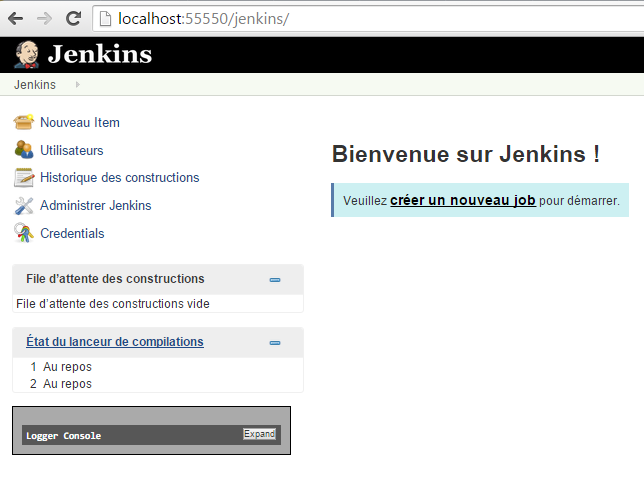
\includegraphics[width=\textwidth]{images/firstJenkinsWhenGenerateTheSkeletonPlugin.png}
  \caption{Jenkins à l'exécution de la commande maven qui l'encapsule}
	\label{figure:firstJenkinsWhenGenerateTheSkeletonPlugin}
\end{figure}



\subsubsection{Essaie du squelette du plugin}
Jenkins se redémarre et voilà notre plugin intégré à celui-ci. Nous pouvons aller voir l'écran de configuration générale et vérifier que le fichier global.jelly a bien été ajouté, on coche la case maintenant disponible pour valider la mise en \oe{}uvre du plugin. Maintenant configurons un projet au hasard et ajoutons une étape pré build, nous aperçevons un item s'appelant \textquote{say hello world}, sélectionnons-le et remplissons le champ de texte qui appara\^{i}t. Compilons le projet et regardons la sortie console, au début nous voyons notre texte qui s'est affiché.\\
Nous avons donc un plugin qui permet de dire quelque chose en début ou fin de build. 



\section{Implémentation de la base du nouveau plugin}

Nous avons donc un plugin qui étend le comportement lors des builds que Jenkins exécute, ceci grâce au point d'extension Builder.\\
Jenkins possède beaucoup de points d'extensions et, à cette étape, il faut déterminer lequel, ainsi que la classe à étendre! Dans le cas où aucun point d'extension ne correspond, il est très facile d'en créer un en suivant la documentation. Autrement, nous pouvons nous inspirer du plugin Radiator et regarder quelle classe il étend.\\
En parcourant la liste des points d'extensions disponibles, nous pouvons trouver \emph{View}, dont l'une de ses implémentations est \emph{ListView}; sa description étant \textquote{Displays Jobs in a flat list view}. Notre objectif étant d'afficher les Jobs, cette solution semble correspondre. De plus, en observant la javadoc, on peut trouver la méthode nous donnant accès au projet associés à la vue (figure \ref{figure:listviewJavaDoc} page \pageref{figure:listviewJavaDoc}).

\begin{figure}[!h]
  \centering
      
\includegraphics[width=\textwidth]{images/listviewJavaDoc.png}
  \caption{Extrait de la javadoc de la classe ListView}
	\label{figure:listviewJavaDoc}
\end{figure}



\subsection{Import du code dans l'IDE}
J'ai expérimenté deux IDE pour développer le plugin : Eclipse puis NetBeans.\\
En utilisant Eclipse, j'ai rencontré beaucoup de problèmes liés aux configurations maven et d'Eclipse, de telle sorte qu'à un moment donné je me trouvais obligé de compiler le code via Jenkins, de récupérer le .hpi en local pour l'intégrer ensuite à Jenkins!
Le cycle de développement était le suivant :

\begin{enumerate}
	\item Implémentation du code sous Eclipse
	\item Compilation du code grâce à maven (ou Jenkins!) et génération du fichier .hpi
	\item Désinstallation du plugin de Jenkins + redémarrage
	\item Installation du nouveau plugin sur Jenkins + redémarrage
	\item Test du plugin
\end{enumerate}
L'utilisation de Netbeans (et de son plugin Jenkins) évite de passer par toutes ces étapes car il suffit de cliquer sur run pour exécuter le plugin et sur debug pour le debugger. Cela facilite l'implémentation du code et, surtout, permet de se focaliser sur les problèmes liés au plugin plutôt qu'à ceux liés aux outils de développement.\\


\subsection{Implémentation de la base}

Avant de pouvoir vraiment travailler à l'implémentation des fonctionnalités du logiciel, il faut encore savoir où écrire le code et comment nommer ses fichier. Une fois que Jenkins à localiser l'annotation précisant qu'il s'agit d'un plugin, il utilise une convention de nommage pour accéder aux différents fichiers d'aide ou de configuration. Pour savoir comment doit se nommer mon fichier de configuration, je vais chercher où se trouvent les fichiers de configuration de Listview dans le code de jenkins-core. Ce qui me m'offrira la possiblité d'implémenter ma propre configuration. L'arborescence de ce fichier est illustrée figure \ref{figure:listviewJavaDoc} page \pageref{figure:listviewJavaDoc}. Il convient maintenant de copier ce fichier et de le coller dans le répertoire \emph{ressources} de notre projet.


\begin{figure}[!h]
  \centering
      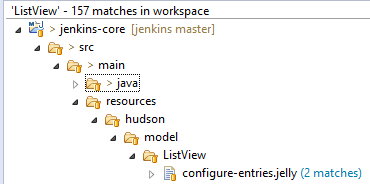
\includegraphics{images/listviewSearch.png}
  \caption{Chemin d'accès au fichier de configuration par défaut}
	\label{figure:listviewSearch}
\end{figure}

Maintenant que l'on peut personnaliser la configuration du plugin, il faut pouvoir faire de même avec l'affichage de la vue. Nous allons donc créer un nouveau fichier \emph{main.xml} qui contiendra le code de l'interface graphique du plugin.\\

Après quelques tests rapides, on s'aperçoit que beaucoup de code, css ou JavaScript, est exécuté lorsque l'on accède à la page. Il faut donc réinitialiser le css pour travailler dans de bonnes conditions. Premièrement, on supprime l'affichage du header, footer et side-panel de Jenkins (cf figure \ref{figure:cssInit} page \pageref{figure:cssInit}) et deuxièmement on supprime l'affichage du side-panel, après chargement de la page (cf figure \ref{figure:cssInitJS} page \pageref{figure:cssInitJS}).\\

\begin{figure}[!h]
  \centering
      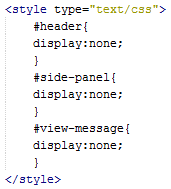
\includegraphics{images/cssInit.png}
  \caption{Initialisation des css avant chargement}
	\label{figure:cssInit}
\end{figure}

\begin{figure}[!h]
  \centering
      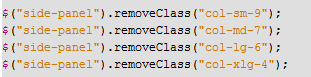
\includegraphics{images/cssInitJS.png}
  \caption{Initialisation des css après chargement}
	\label{figure:cssInitJS}
\end{figure}


\section{Travail réalisé}

\subsection{Caractéristiques du logiciel}%Et mon cahier des charges, il est où?????
changer couleur background et police
regroupe par prefixe
priorise les status
va chercher info dans archive
....




\begin{figure}[!h]
  \centering
      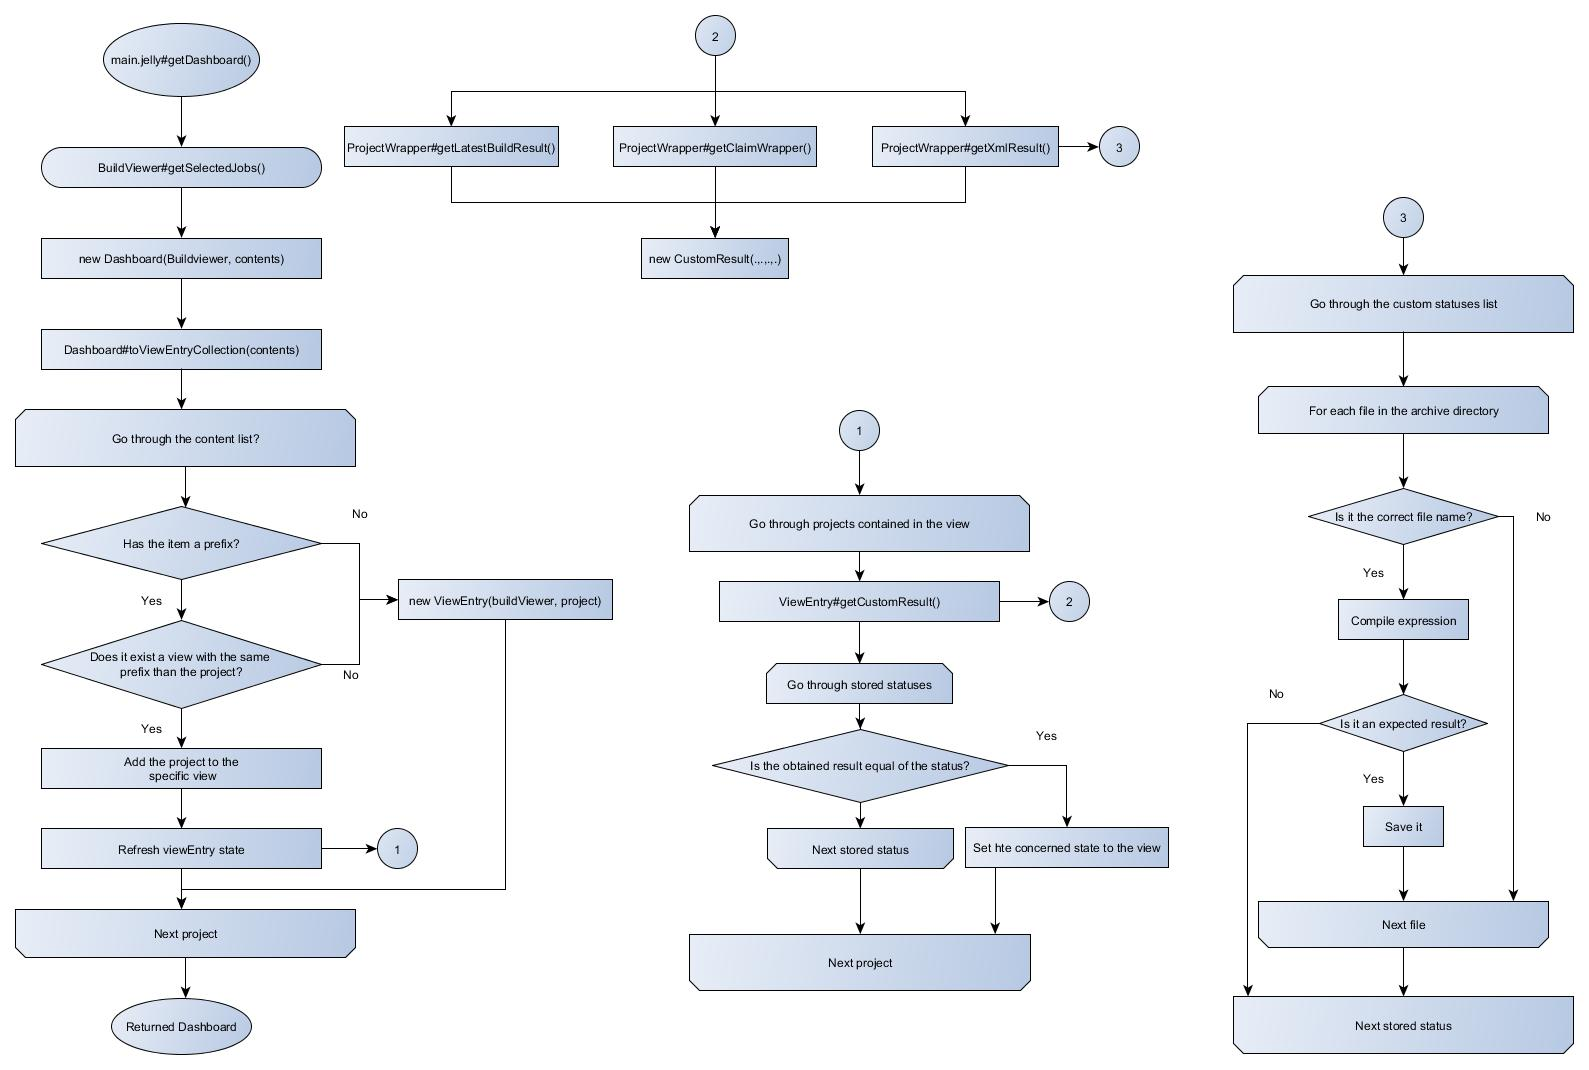
\includegraphics[width=\textheight,angle=90]{images/dashboardGenesis.jpg}
  \caption{Algorithme de création du Dashboard}
	\label{figure:dashboardGenesis}
\end{figure}


\begin{figure}[!h]
  \centering
      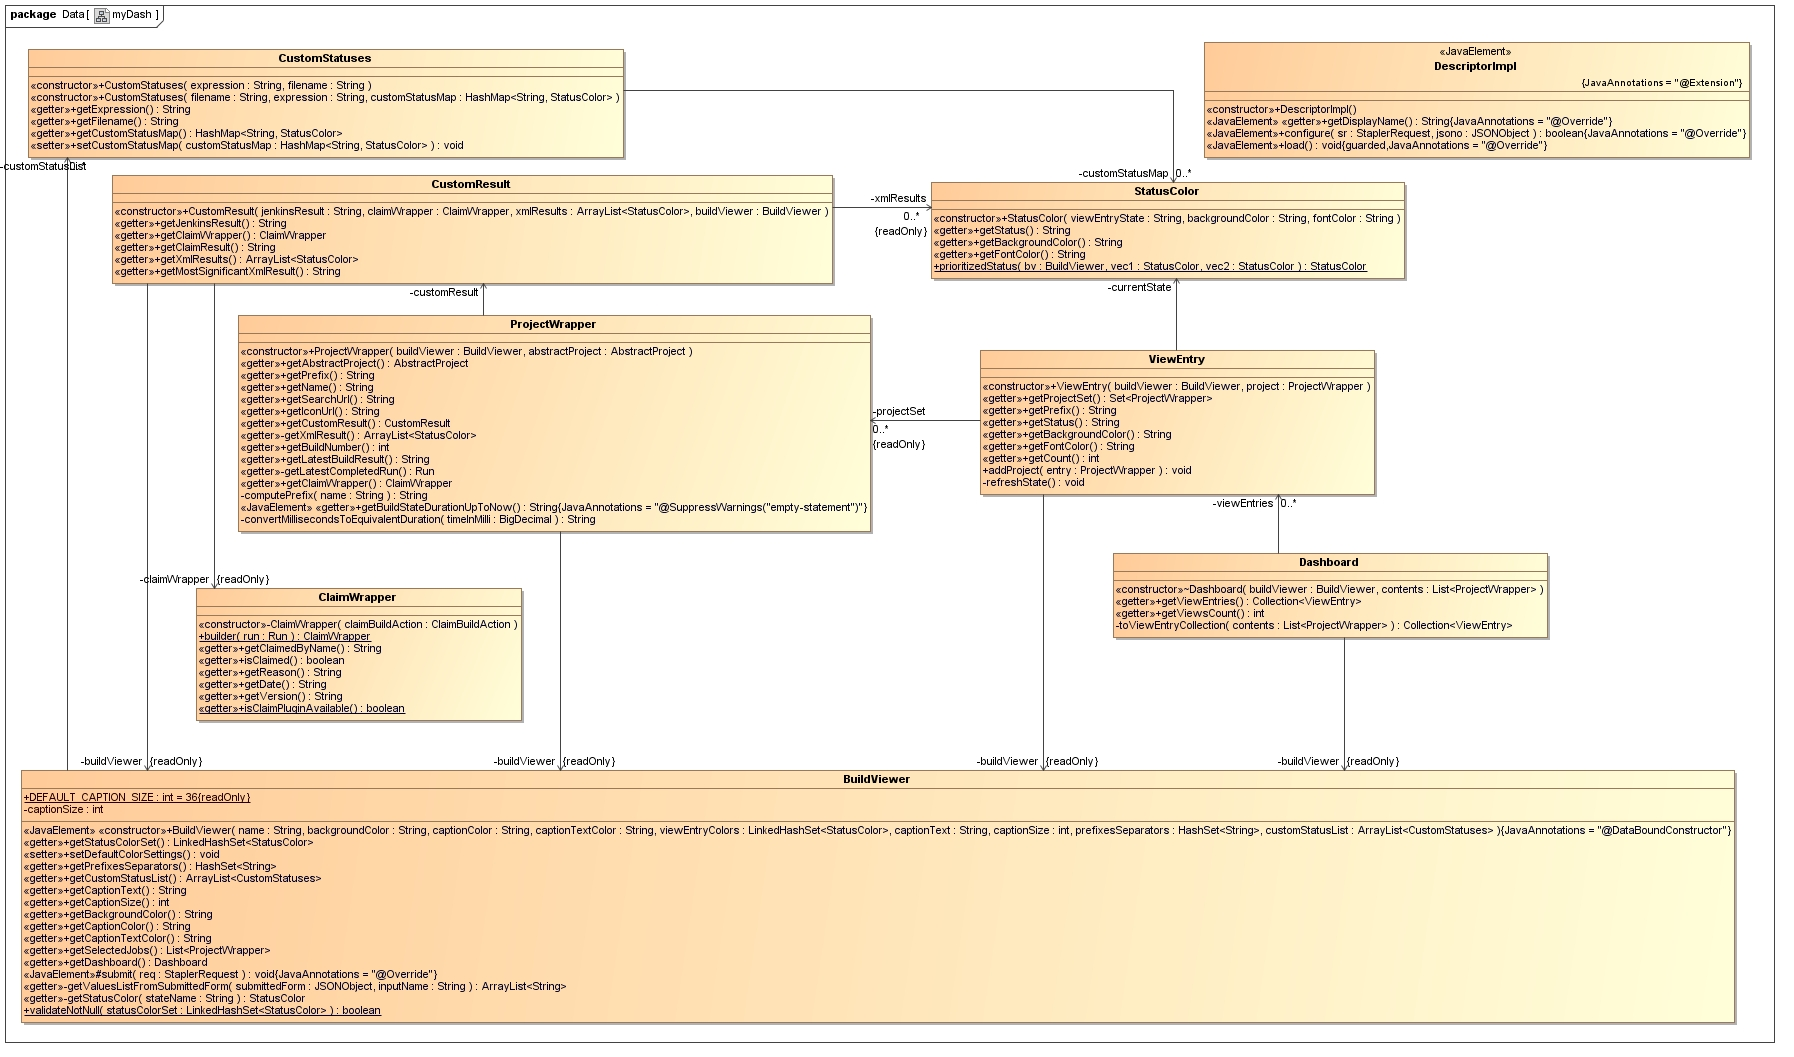
\includegraphics[width=\textheight,angle=90]{images/myDash.jpg}
  \caption{Diagramme de classe du plugin réalisé}
	\label{figure:myDash}
\end{figure}


%\chapter*{Bilan}
\addcontentsline{toc}{chapter}{Bilan}
\markboth{Bilan}{}

Les diff\'{e}rentes missions qu'il m'a \'{e}t\'{e} donn\'{e} d'effectuer m'ont d'abord permis de participer activement \`{a} l'activit\'{e} de l'entreprise et de me retrouver dans la peau d'un ing\'{e}nieur qualit\'{e}, me posant des questions n\'{e}cessitant une vrai compr\'{e}hension du produit et du recul par rapport \`{a} mes objectifs.\\

Lorsque mes coll\`{e}gues n'avaient pas le temps de s'occuper de ce qu'ils voulaient, je me suis vu affecter leurs t\^{a}ches. Me pencher sur le genre de travaux que l'on donne aux ing\'{e}nieurs a \'{e}t\'{e} pour moi une marque de reconnaissance. Mais paradoxalement cela a aussi \'{e}t\'{e} \`{a} l'origine de remises en question \textquote{En serai-je capable?}, \textquote{Ai-je les connaissances requises?}, \textquote{Vais-je r\'{e}ussir dans le temps imparti?}.\\

Le d\'{e}veloppement d'un plugin Jenkins a \'{e}t\'{e} une vraie \'{e}tapes dans ma carri\`{e}re de d'ing\'{e}nieur, un pied de pos\'{e} dans la r\'{e}alit\'{e} du d\'{e}veloppement logiciel mais surtout du logiciel libre. Signifiant que j'ai particip\'{e} activement \`{a} l'\'{e}volution de ce logiciel open-source et communautaire. J'ai communiqu\'{e} avec le concepteur de l'ancien plugin, que le mien remplace, et c'est avec plaisir qu'il m'a apport\'{e} les r\'{e}ponses \`{a} mes questions. Mon plugin n'est, pour l'heure, pas encore sur le repository officiel mais cela est en discussion. Cette \'{e}ventualit\'{e} permettrai \`{a} n'importe quel utilisateur de Jenkins d'essayer mon plugin et de l'adopter, ou de le rejeter. Bien \'{e}videmment, le rendre disponible publiquement le mettrais \`{a} l'\'{e}preuve d'utilisation pour lesquelles il n'avait pas \'{e}t\'{e} pr\'{e}vu initialement. Il est donc certain que des bugs seront trouv\'{e}s, autrement dit, le livrer sur le repository officiel n\'{e}cessite de le maintenir et de rester disponible pour la maintenance, l'\'{e}volution et pour r\'{e}pondre aux questions des utilisateurs.\\

Techniquement, j'ai eu la chance de pouvoir me pencher sur plusieurs sujets diff\'{e}rents, tenant de domaines techniques diff\'{e}rents et \`{a} des fins diff\'{e}rentes. En d\'{e}veloppant les tests j'ai impl\'{e}ment\'{e} du code Java, non pour apprendre une technologie, mais pour r\'{e}ussir \`{a} faire quelque chose, me focalisant ainsi sur l'objectif et les performances plut\^{o}t que sur la mani\`{e}re.\\

De tout ce que j'ai pu faire lors de ce contrat, seule une petite partie de ce que j'ai appris \`{a} l'\'{e}cole m'a \'{e}t\'{e} n\'{e}cessaire, bien qu'essentielle. Je me suis vu aborder des probl\'{e}matiques et des technologies dont j'avais, tout au plus, vaguement entendu parl\'{e}. J'ai donc adopt\'{e} une vrai m\'{e}thode de travail o\`{u} ce qui compte n'est pas la maitrise de telle ou telle technologie, comme en \'{e}cole d'ing\'{e}nieur, mais de proposer une solution fiable et performante, quelle que soit le moyen utilis\'{e}. Ce faisant je me suis pos\'{e} les vraies questions qui concernent v\'{e}ritablement un ing\'{e}nieur : \textquote{Quels sont les diff\'{e}rents moyens de r\'{e}soudre ce probl\`{e}me?}, \textquote{Quels sont les diff\'{e}rents avantages et inconv\'{e}nients?}, \textquote{Quelles sont les normes, les n\'{e}cessit\'{e}s, les limitions juridiques?}, \textquote{Quelles sont les personnes comp\'{e}tentes qui pourrons me donner des informations primordiales pour mon projet?}.\\






D'un point de vue personnel, ce qui a \'{e}t\'{e} un frein au d\'{e}but de mon contrat de professionnalisation f\^{u}t, d'une part, mon acharnement \`{a} vouloir tout comprendre dans les d\'{e}tails sans que cela soit n\'{e}cessaire, et d'autre part, \`{a} ne pas me tourner vers les personnes comp\'{e}tentes qui auraient pu me conseiller, r\'{e}duisant ainsi des p\'{e}riodes d'\'{e}tudes de plusieurs jours \`{a} quelques heures. Je regrette de ne pas avoir \'{e}t\'{e} suffisamment demandeur d'informations, d\'{e}sirant faire le mieux possible, le plus vite et sans soutien ce que l'on attendait de moi, ainsi, je n'ai pas appris tout ce que j'aurai pu.\\

Si c'\'{e}tait \`{a} refaire je ne me jetterai pas tout suite dans l'\'{e}laboration de ma strat\'{e}gie pour arriver au bout de ma mission, mais passerai beaucoup plus de temps \`{a} me diriger vers les autres pour discuter des contours de mon projets, des probl\`{e}mes potentiels et des solutions d\'{e}j\`{a} existentes; chose que je faisait beauxoup plus facilement plus tard, mon contrat arrivant \`{a} son terme.\\


Le temps que j'ai pass\'{e} dans cette entreprise est une immense fiert\'{e} dont je n'h\'{e}siterai pas \`{a} vendre les m\'{e}rites. Parce que c'est dans un contexte internationnal que j'ai particip\'{e} au d\'{e}veloppement du framework de test, et parce que c'est pour le leader de la BI que j'ai d\'{e}velopp\'{e} un outil open-source, utilis\'{e} quotidiennement, de reporting des builds. Ce contrat de professionnalisation \`{a} \'{e}t\'{e} une exp\'{e}rience exceptionnellement riche, tant par ce que j'ai appris \`{a} faire ou \`{a} \^{e}tre, que par les nombreuses connaissances techniques que j'ai pu accumuler. 




%\chapter*{Conclusion}
\addcontentsline{toc}{chapter}{Conclusion}
\markboth{Conclusion}{}
Mon contrat professionnel à SAP fût une expérience remarquable tant par la valeur de l'équipe que j'ai intégré que par les missions que je me suis vu effectuer. 

M'a permi de découvrir l'environnement complexe d'une multinationnale et les outils mis à disposition des employés pour permettre une bonne communication au sein de l'entreprise.
J'ai pu me rendre compte de l'ampleur d'un projet comme WebI ainsi que toutes les ressources impliquées dans la conduite de celui-ci.

Les apports de ma mission pour l'entreprise ?
L'avenir du projet dans l'entreprise.
Un prolongement éventuel? Une proposition refusée


les apports de la mission pour l'ent
les prolongements du travail
l'avenir du projet
\cleardoublepage% le corps du document est terminé

\appendix
\pagestyle{back}
%\newgeometry{left=1cm,right=1cm,top=0cm,bottom=2cm}

\chapter{Les niveaux de test}

\begin{figure}[!h]
  \centering
      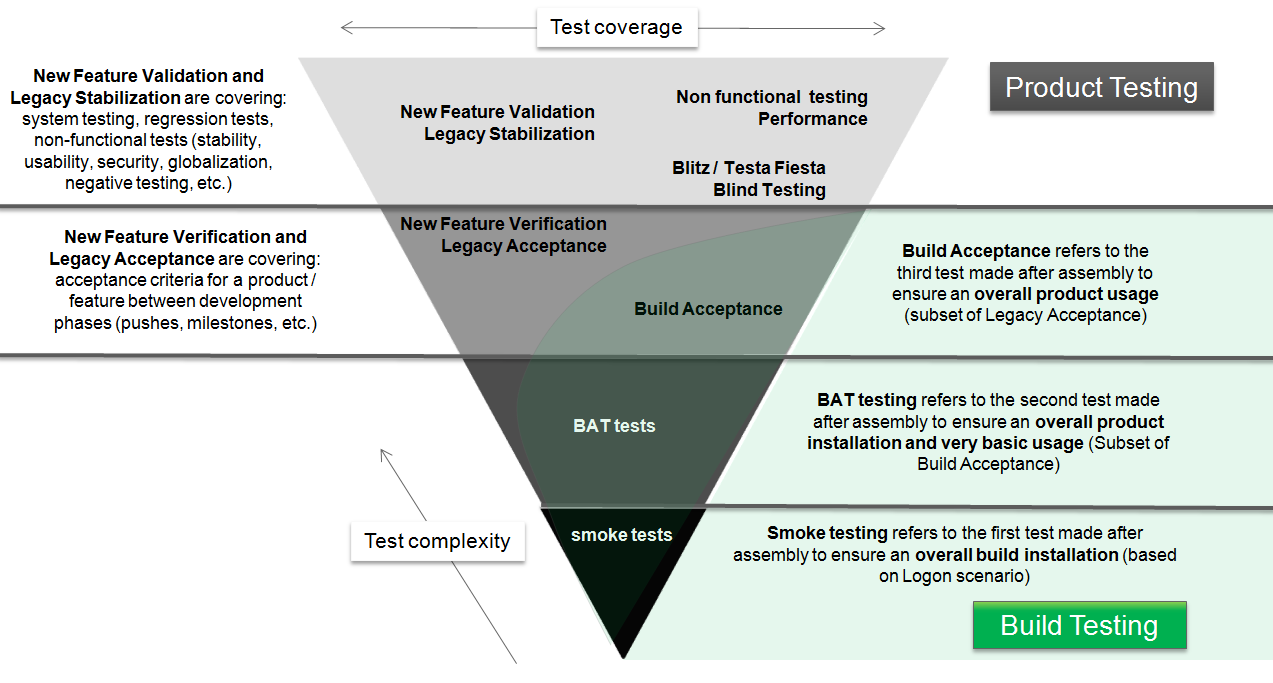
\includegraphics[width=0.7\textheight,angle=90]{images/TestingLevels.png}
  \caption{Les diff\'{e}rents niveaux de test}
	\label{figure:testLevels}
\end{figure}

\clearpage
\restoregeometry
%\newgeometry{left=1cm,right=1cm,top=0cm,bottom=2cm}

\chapter{R\'{e}sultats quotidiens des tests}\label{pdf:automationResults}


%\begin{figure}[!ht]
%  \centering
%      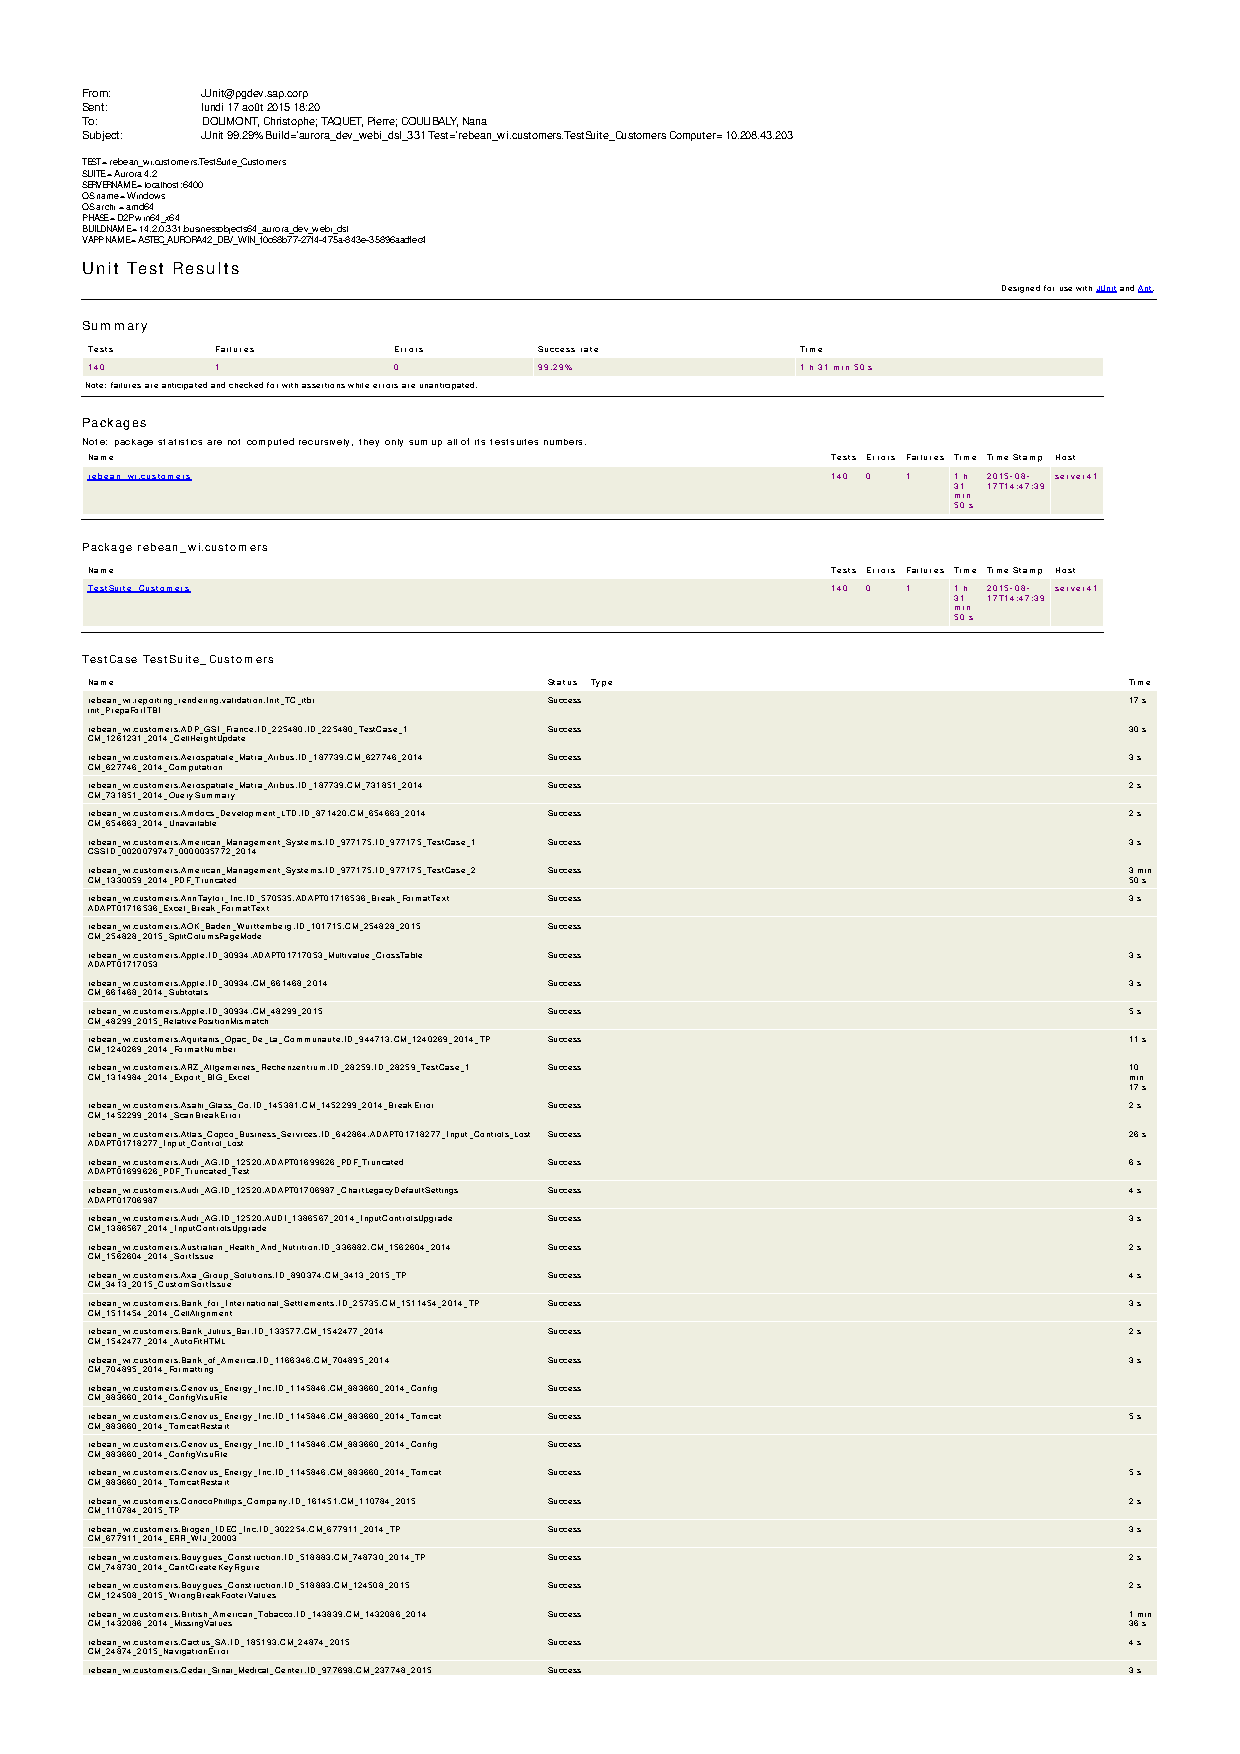
\includegraphics{images/AutomationResults.pdf}
%	\label{figure:AutomationResults}
%\end{figure}

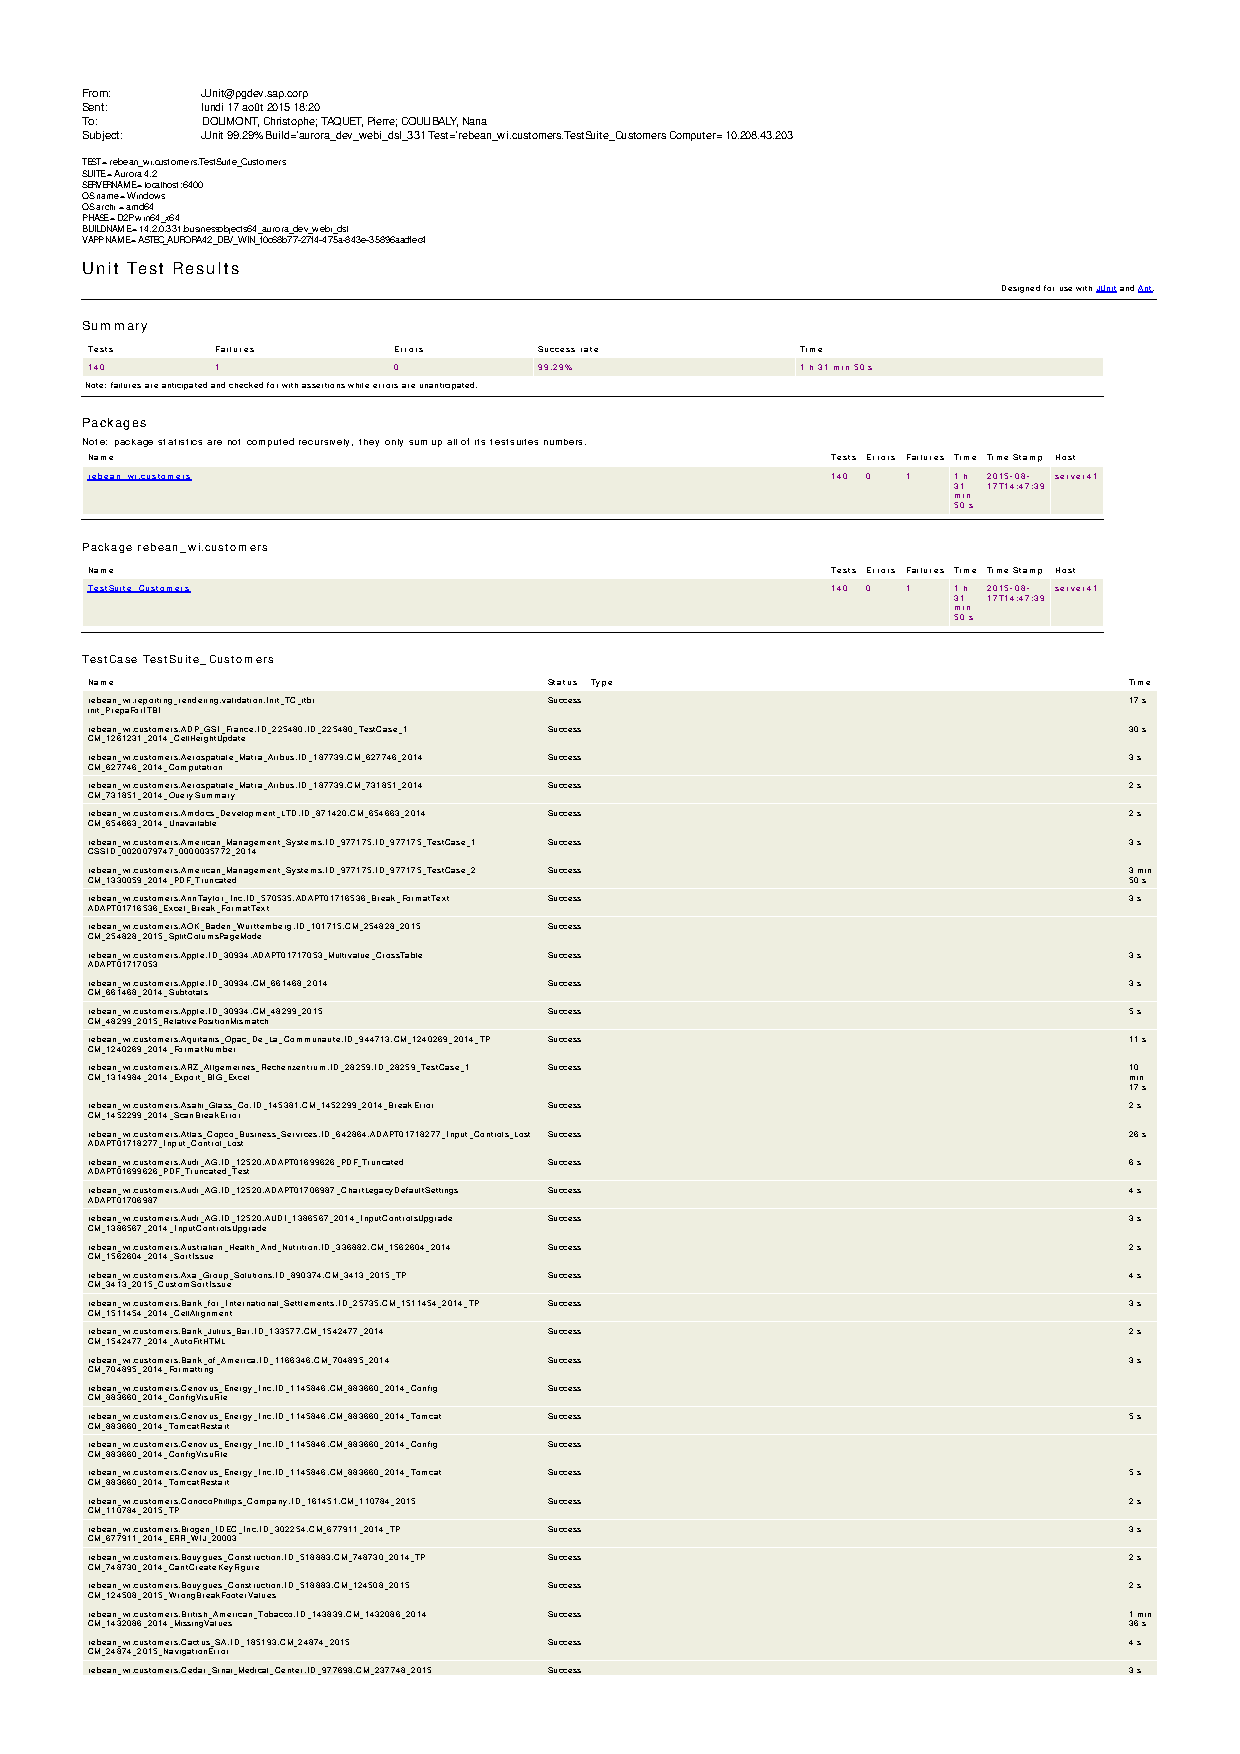
\includepdf[pages=-,scale=0.9,pagecommand={}]{images/AutomationResults.pdf}

\restoregeometry
%\newgeometry{left=1cm,right=1cm,top=0cm,bottom=2cm}

\chapter{Tous les tests impl\'{e}ment\'{e}s}\label{pdf:ImplementedTestsList}


%\begin{figure}[!ht]
%  \centering
%      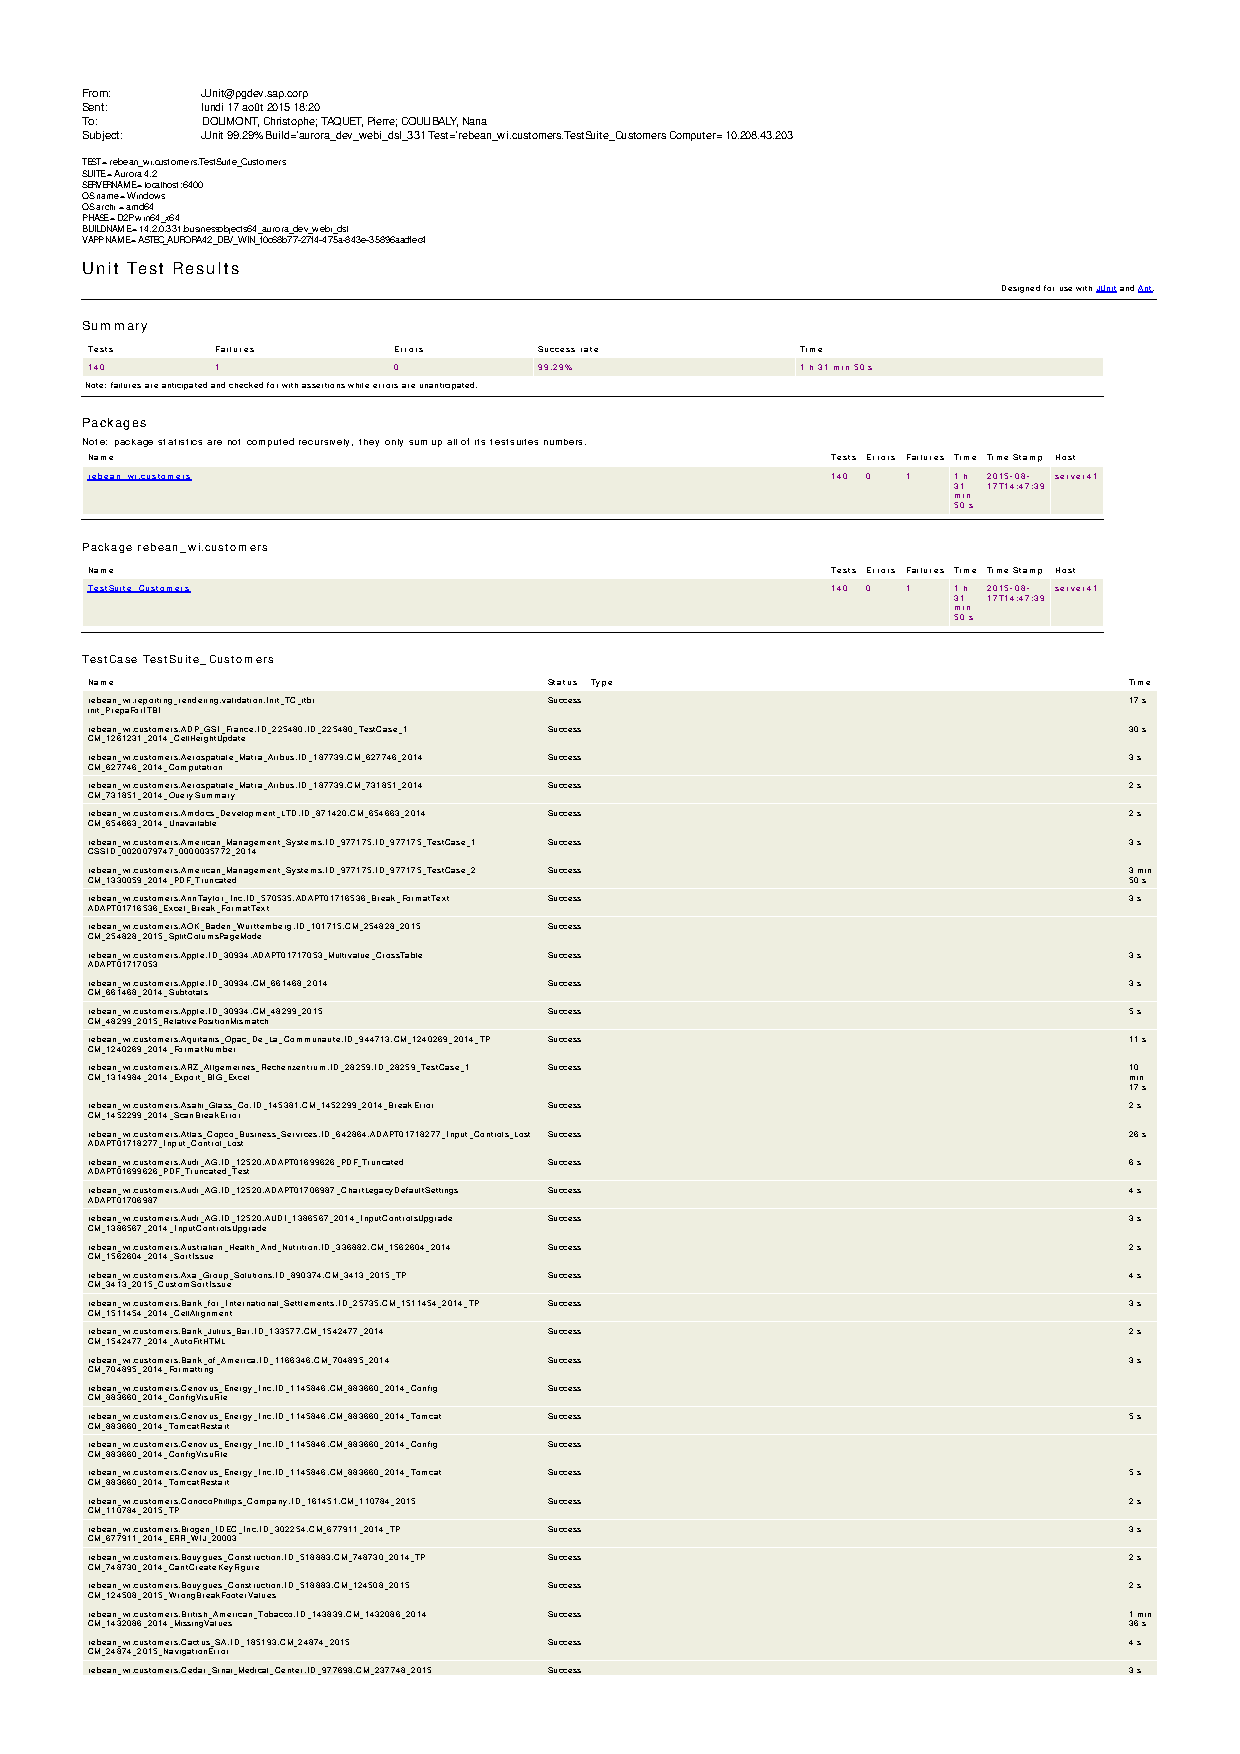
\includegraphics{images/AutomationResults.pdf}
%	\label{figure:AutomationResults}
%\end{figure}

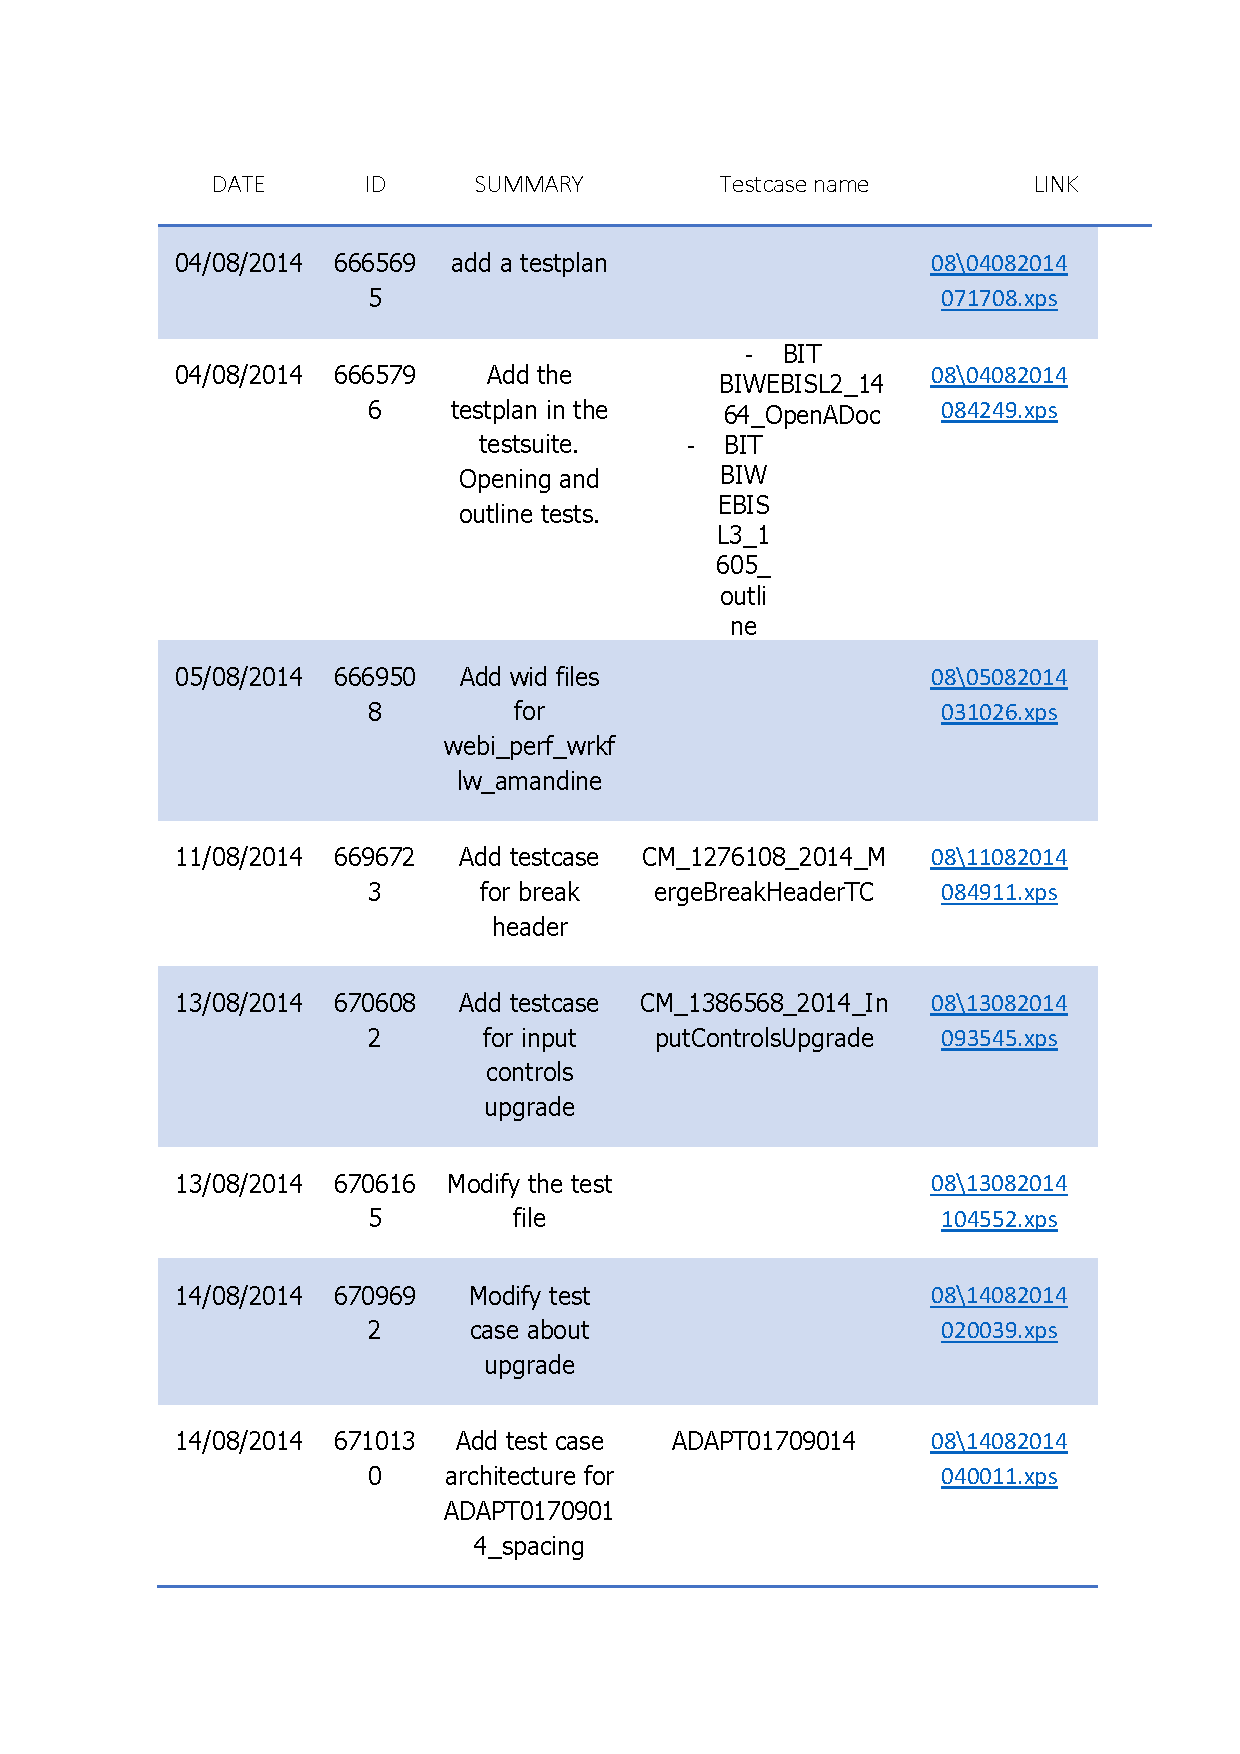
\includepdf[pages=-,scale=0.9,pagecommand={}]{images/ImplementedTestsList.pdf}

\restoregeometry
%\chapter{Les bases pour comprendre Jenkins}\label{annexe:jenkinsBasis}

cf annexe diff\'{e}rence entre job et projet http://jenkins-ci.361315.n4.nabble.com/Is-it-called-quot-Project-quot-or-is-it-called-quot-Job-quot-td4628610.html\\


cf annexe status JUnit vs status Jenkins\\

						-	https://wiki.jenkins-ci.org/display/JENKINS/Terminology
						
						
!!!! La base de l'impl\'{e}mentation d'un plugin


https://wiki.jenkins-ci.org/display/JENKINS/Extend+Jenkins


https://wiki.jenkins-ci.org/display/JENKINS/Plugin+tutorial
%\chapter{Maven}\label{annexe:maven}


C'est quoi?

Concr\`{e}tement \c{c}a sert \`{a} quoi?

Comment \c{c}a s'installe?

Exemple d'utilisation : g\'{e}n\'{e}ration de skeleton du plugin Jenkins



%\chapter{Mail re\c{c}u d'un mauvais push}\label{annexe:crashedBuildBecauseOfMe}


	\begin{figure}[!h]
  \centering
      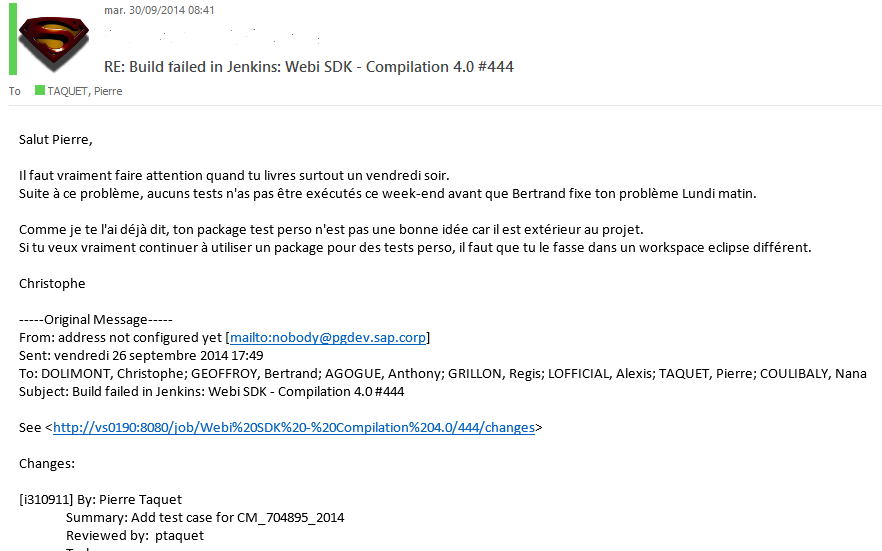
\includegraphics[width=\textwidth]{images/crashedBuildBecauseOfMe.png}
  \caption{Capture d'\'{e}cran du r\'{e}sultat de ma mauvaise manipulation}
\end{figure}

%\chapter{Maven}\label{annexe:DParameters}

explication des paramttreds -d
\newgeometry{left=1cm,right=1cm,top=0cm,bottom=2cm}

\chapter{Fiche d'information de SAP}\label{annexe:SAP-Corporate-Fact-Sheet}



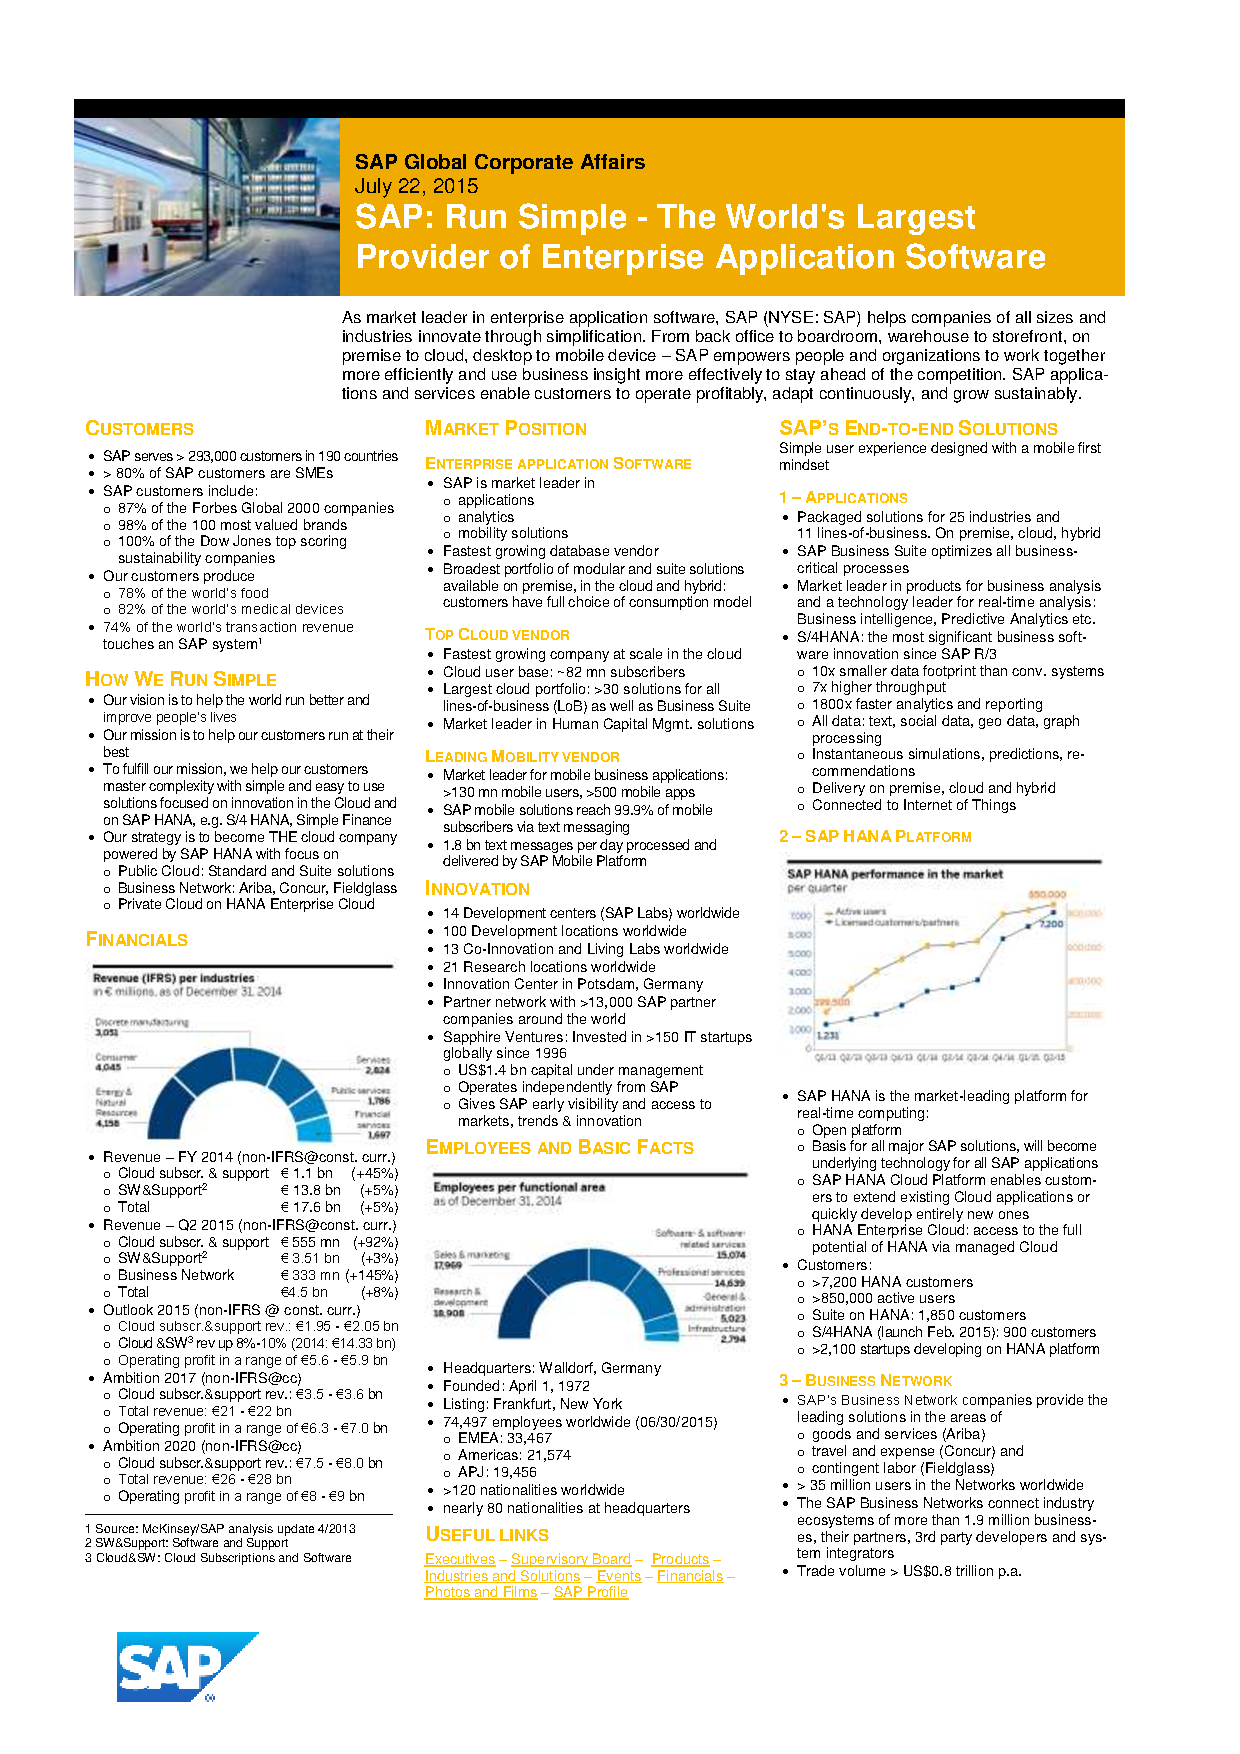
\includepdf[pages=-,scale=0.9,pagecommand={}]{images/SAP-Corporate-Fact-Sheet.pdf}\thispagestyle{empty}


\restoregeometry


\chapter{Exemple d'une sortie console}\label{annexe:sortieConsole}

\lstinputlisting{scripts/sortieConsole.txt}




\backmatter
%\printindex
%\addcontentsline{toc}{chapter}{Index}

%\glsaddall
\printglossaries
\addcontentsline{toc}{chapter}{Glossaire}

%\printnomenclature
%\addcontentsline{toc}{chapter}{Liste des abréviations, des sigles et des symboles}

%\cite{JenkinsTerminology}%\cite[p.~215]{citation01}
%\cite{*}

%\printbibliography
%\addcontentsline{toc}{chapter}{Bibliographie}

%\begin{thebibliography}{9}

%\bibitem{lamport94}
%  Leslie Lamport,
%  \emph{\LaTeX: a document preparation system},
%  Addison Wesley, Massachusetts,
%  2nd edition,
%  1994.%%

%\end{thebibliography}
%@ONLINE{JenkinsTerminology,
%author = {Community, Open source},
%title = {Terms used in Jenkins},
%month = {feb},
%year = {2015},
%url = {https://wiki.jenkins-ci.org/display/JENKINS/Terminology}
%}





%\listoffigures
%\addcontentsline{toc}{chapter}{Table des figures}

%\listoftables
%\addcontentsline{toc}{chapter}{Liste des tableaux}

\tableofcontents%table des matières plus complète   <<<<<<<<<  Important pour le sommaire plus haut!
\addcontentsline{toc}{chapter}{Table des matières}%ajout de la table des matières dans la table des matières !


%\clearpage
\ifodd\thepage\hbox{}\newpage\else\fi%si page paire ou impaire
\parindent=0pt

\newgeometry{left=2cm,right=3cm}
\restoregeometry

\thispagestyle{empty}

%
\begin{center}
{\Large \textbf{Abstract}}
\end{center}



This report focuses on my work for the duration of my internship. This content is divided into four areas.
The first part provides information on the firm in which I worked and the following three parts describe each of my assignments.
The common point of all is the Java development but for different purposes.




The first assignment was Java test development based on an internal Framework.
It was a very interesting part because of the wealth of expertise and experience found in the project which I integrated.
During this period I accumulated a large amount of knowledge, concerning the Framework itself or the Java.

The second assignment was complement an existing Java class to adapt its behavior to a new used tool.
It was a hard part due to the fact there are many studies to be done for relatively little Java code.
I had to integrate my Java implementation into an already existing code and I was very formative.

The third assignment, and also the most interesting and formative, was the Jenkins plug-in development.
I studied Jenkins and the way to develop a plug-in for a long time. Next, I had to gradually had new features for the purpose of obtain the expected plugin.
The other thing was the human side and the teamwork. Indeed I reported weekly the project progresses and work in pair.



My employer was SAP France, firstly I worked in Levallois-Perret, next to Paris, from July to mid-February. Next, SAP moved towards to a larger building, still in the same town. I worked there until end of September.


It was with a great pleasure to spent my time in there. I learned many things during this internship period, I was able to use new technologies and unknown tools. 


\vspace*{\stretch{2}}

\hrulefill
\begin{center}
{\Large \textbf{Keywords}}
\end{center}
\hrulefill





\begin{center}
Software tester\\
JavaEE\\
Agile\\
Jenkins\\
Plugin\\
\end{center}

\end{document}
